\documentclass[11pt, chapterprefix=true]{scrbook}\usepackage[]{graphicx}\usepackage[]{color}
%% maxwidth is the original width if it is less than linewidth
%% otherwise use linewidth (to make sure the graphics do not exceed the margin)
\makeatletter
\def\maxwidth{ %
  \ifdim\Gin@nat@width>\linewidth
    \linewidth
  \else
    \Gin@nat@width
  \fi
}
\makeatother

\definecolor{fgcolor}{rgb}{0.345, 0.345, 0.345}
\newcommand{\hlnum}[1]{\textcolor[rgb]{0.686,0.059,0.569}{#1}}%
\newcommand{\hlstr}[1]{\textcolor[rgb]{0.192,0.494,0.8}{#1}}%
\newcommand{\hlcom}[1]{\textcolor[rgb]{0.678,0.584,0.686}{\textit{#1}}}%
\newcommand{\hlopt}[1]{\textcolor[rgb]{0,0,0}{#1}}%
\newcommand{\hlstd}[1]{\textcolor[rgb]{0.345,0.345,0.345}{#1}}%
\newcommand{\hlkwa}[1]{\textcolor[rgb]{0.161,0.373,0.58}{\textbf{#1}}}%
\newcommand{\hlkwb}[1]{\textcolor[rgb]{0.69,0.353,0.396}{#1}}%
\newcommand{\hlkwc}[1]{\textcolor[rgb]{0.333,0.667,0.333}{#1}}%
\newcommand{\hlkwd}[1]{\textcolor[rgb]{0.737,0.353,0.396}{\textbf{#1}}}%
\let\hlipl\hlkwb

\usepackage{framed}
\makeatletter
\newenvironment{kframe}{%
 \def\at@end@of@kframe{}%
 \ifinner\ifhmode%
  \def\at@end@of@kframe{\end{minipage}}%
  \begin{minipage}{\columnwidth}%
 \fi\fi%
 \def\FrameCommand##1{\hskip\@totalleftmargin \hskip-\fboxsep
 \colorbox{shadecolor}{##1}\hskip-\fboxsep
     % There is no \\@totalrightmargin, so:
     \hskip-\linewidth \hskip-\@totalleftmargin \hskip\columnwidth}%
 \MakeFramed {\advance\hsize-\width
   \@totalleftmargin\z@ \linewidth\hsize
   \@setminipage}}%
 {\par\unskip\endMakeFramed%
 \at@end@of@kframe}
\makeatother

\definecolor{shadecolor}{rgb}{.97, .97, .97}
\definecolor{messagecolor}{rgb}{0, 0, 0}
\definecolor{warningcolor}{rgb}{1, 0, 1}
\definecolor{errorcolor}{rgb}{1, 0, 0}
\newenvironment{knitrout}{}{} % an empty environment to be redefined in TeX

\usepackage{alltt}
\usepackage[colorlinks=true]{hyperref}
%\usepackage[lmargin=3cm, rmargin=2cm, showframe]{geometry}    % See geometry.pdf to learn the layout options. There are lots.
% \usepackage[lmargin=3cm, rmargin=2cm]{geometry}
\usepackage[lmargin=4cm, rmargin=2cm]{geometry}
\usepackage{pict2e}
\usepackage[english]{babel}
\definecolor{lred}{rgb}{1,0.5,0}
\definecolor{lyellow}{rgb}{.94, .9, .55}
\definecolor{lgray}{rgb}{.83, .83, .83}
% \usepackage[parfill]{parskip}    % Activate to begin paragraphs with an empty line rather than an indent

\geometry{letterpaper}    % ... or a4paper or a5paper or ...
%\geometry{landscape}     % Activate for for rotated page geometry
\usepackage{graphicx}
\setkeys{Gin}{width=\linewidth}
\usepackage{amssymb}
\usepackage{amsmath}
\usepackage{epstopdf}
\usepackage{exsol, fancyvrb}                % Provides exercises and solutions.  See https://ctan.org/pkg/exsol.
\usepackage{color}
\usepackage{verbatim}
\usepackage{changepage}
\usepackage{url}
\usepackage[authoryear]{natbib}
\usepackage{makeidx}

\DeclareGraphicsRule{.tif}{png}{.png}{`convert #1 `dirname #1`/`basename #1 .tif`.png}

\title{{\Huge{STAT 1600 \\ Statistics and Data Analysis }}}
\subtitle{{\huge{Course Pack}}}
\author{Statistics Computational Lab (SCL)}
\date{2018 - 2019 Edition}  % Activate to display a given date or no date

%\title{STAT 1600 \\ Statistics and Data Analysis }
%\author{Department of Statistics \\ Western Michigan University}
%\date{}% Activate to display a given date or no date
\KOMAoptions{parskip=half}
\makeindex
\IfFileExists{upquote.sty}{\usepackage{upquote}}{}
\begin{document}

\maketitle

%\section{}
%\subsection{}

\begin{center} \textbf{Acknowledgements:}
\end{center}

Carrie McKean, Srikanthmadhavan Aravamuthan, Cody Weiss, Carson Miller,  Rudie \\ Desravines, Eunice Ampah, Joseph Billian,  Ian Kapenga, and Mr. Loren L. Heun assisted with  this material.

\vspace{11cm}

Copyright 2017 by The Department of Statistics at Western Michigan University.

All rights reserved.

Reproductions or translation of any part of this work beyond that permitted by Sections 107 and 108 of the 1976 United States Copyright Act without permission of the copyright owner is unlawful.

A general introduction to statistics with an emphasis on data analysis and graphical presentation. Extensive use will be made of the computer to prepare results. Topics may include: data collection, sampling and experimentation, measurement issues, descriptive statistics, statistical graphics, normal distribution, cross-classified data, correlation and association, formal statistical inferences, and resampling methods.



\overfullrule=1cm

\tableofcontents



%!Rnw root = ../../Master.Rnw


\chapter{Knowledge and Data}
\label{chap:ch1}

\section{Objectives}

After completing this subsection, students should be able to:

\fbox{\parbox{14cm}{
\begin{itemize}
\item Discern the difference between knowledge and data.
\item Understand the process of acquiring knowledge from the data.
\item Perceive the fallacies of design.
\item Comprehend the meaning of the Type-I and Type-II errors.
\end{itemize}
}}

\section{Knowledge and Data}

There is a difference between what we know, and what we think know.  Are vaccines safe?  Will the new tax rules bring more or less revenue?  Do mandatory seat belt laws save lives?   Will legalizing drugs lead to more addiction?  Do alternative therapies work as effectively as traditional treatments?  Does exercise help prevent illness and are people who generally exercise healthier? Do taller people make more money than shorter people?  \citep{naranjo2018}

Most of these issues can only be settled by looking at data.  What do the data tell us?  Even then, some issues can only be partially answered by at best incomplete data.  In this course, we will discuss some fundamentals of good scientific studies
and data analysis.  In the process, we hope to become better consumers of
information, and better judges of what is true or not true, and what remains to be proven.

\subsection{Building Knowledge Step-by-step}

Scientific studies often go through the following steps.  It might help to read the example in the next section, then read this again.

\subsubsection{1. Conceptualize the problem} \index{Concept}

Suppose that you wish to study and the problem of interest.  The wording is usually broad. The idea at first may be too complex to understand so we look for ways to explain and describe it.

For example, perhaps we are interested in a problem of interest within education.  We will want to clarify and define education.  Are we interested in investigating particular schools or grade levels? Perhaps we want to look at a specific component of education, like science or look at different methods of instruction.   Clarifying specific concepts which we want to investigate and putting this into words helps bring focus to our study.

\subsubsection{2. Operationalize the problem}

As a researcher for your study you also need to come up with ways to narrow in on your problem of interest.  What specifically do you want to measure?  Here we are formulating the specific question we want to answer.  We are also beginning to define our variables.  We will need to know what we can measure to help answer our problem of interest.

Perhaps we are interested in looking at how well students are doing with several different methods of teaching science.  We may look at measures of assessment like how well they did on an exam or overall in a class given the different teaching methodologies.

\subsubsection{3. Design the study}

Here we need to address all the components of how our study will be performed.  We will likely need to identify the population of interest and to obtain a good representative sample of that population.  We will need to figure out how we will select the sample and how many groups we may be comparing.

In our study of science education will we sample from several schools or several districts?  If we take a sample of students from several schools, but from only one state, for example, our population would be students within that state.  If we wanted to define our population as education within the continental U.S., we might need to pull randomly from schools across the U.S.

\subsubsection{4. Collect the data}

In the data collection stage, we must decide what instrument we are using (questionnaire, interview, observation).  Once we have designed our study, we should be able to identify the main variables of interest.  As we collect the data, we are gathering information to help us answer the question we have proposed.

In our example of science education, perhaps we are collecting scores on a particular assessment (exam) to see how well students are learning the material.

\subsubsection{5. Analyze the data}

Using the proper statistical methods and procedures for the data is an important step in the data analysis stage.  Also, checking the assumptions behind these statistical methods is critical.  Are we comparing means?  Proportions?  Are the differences in means/proportions statistically significant?  How do we know if there is a significant difference (if the differences we find are not likely due  to chance)?

In our exploration of teaching science perhaps we are comparing two different methodologies of teaching.  We may then compare the overall means of the two groups.

\subsubsection{6. Conclusions}

Do your results generalize to a larger population?  Check back to see how you defined the population so that you can generalize the results.  Are you concluding cause-and-effect relationship, did you perform an experiment, or did you observe   associations?  In your conclusions, you will also want to identify limits to your study and perhaps suggest further research that may be done in your area.

As we conclude science teaching, perhaps we could only afford to do a smaller study within a particular district.  We could then relate the results of our study, based on our sample of schools, to the population of the entire school district.  We may not be able to make conclusions to the whole state or the U.S. since our sample was not representative of the whole state or the U.S.  Depending on how the study was defined we may have only made observations of the teachers.  If we were investigating two distinct types of instruction, then this falls more within the realm of an experiment.  We, of course, would still need to identify and try to control for confounding variables, which might be difficult.

\subsubsection{7. Disseminate results}

How are we sharing our results?  We need to find the best approach to sharing the results of our study.

Is this information going to be made available to the schools for future educational Improvement?  Are we going to try to publish in a scientific or educational journal?

\subsubsection{The Science Wheel Summarizes the above Steps}

The Wheel of Science  \citep{Wallace1971}
gives us a process to refine our thinking about the nature of social interactions.  See Figure 1.1.  We will define the four parts of the wheel below:  Theory, Hypotheses, Observations, and Empirical Generalizations.

\begin{figure}[htbp]
   \centering

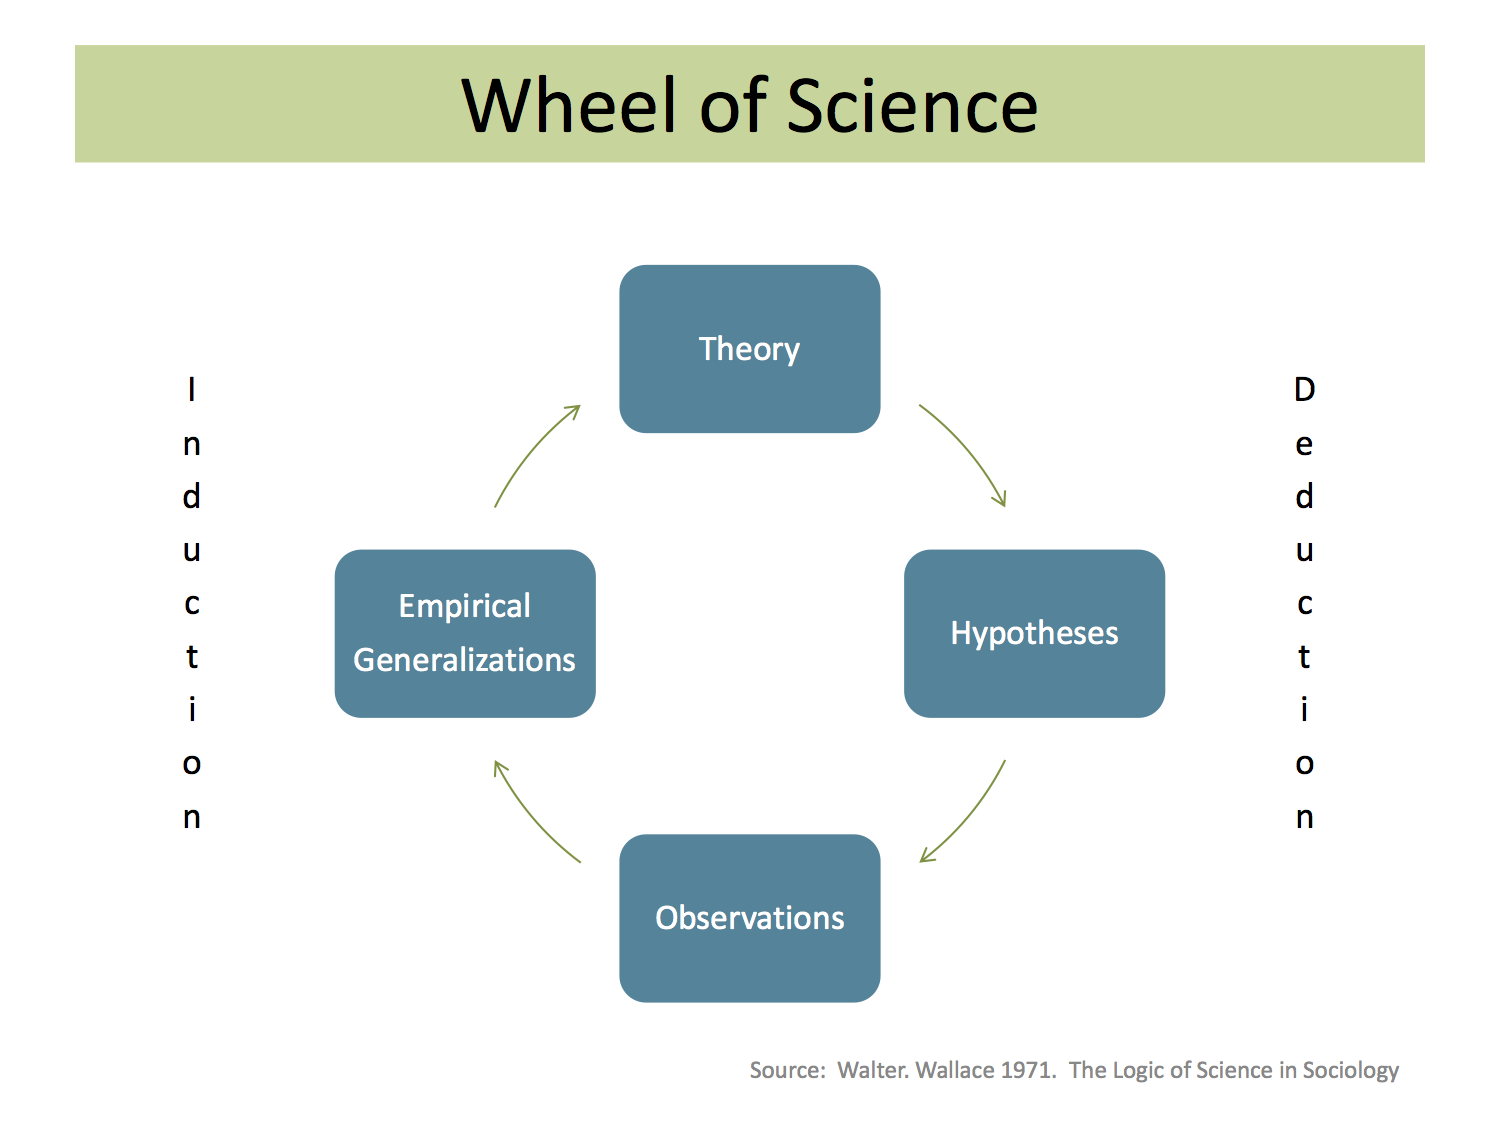
\includegraphics[width=0.5\linewidth]{chapters/Chapter_1/ext_figure/zWheel_Science.png} % requires the graphicx package

   \caption{The Wheel of Science}
   \label{fig:WS}
\end{figure}

\subsection{Example}

Let's look at another example.  Suppose we are interested in comparing the following four popular weight loss diets: Zone (balance between carbohydrates, protein and fat), Atkins (low carbohydrate, high fat, unrestricted calories), LEARN (low fat, based on national guidelines), and Ornish (low fat, high carbohydrate, unrestricted calories).   How would we design a comparison study?

\subsubsection{1.	Conceptualize the problem}

Which weight loss program is most effective?   Which one is the \textit{most healthy}?   Can \\ unrestricted-calorie diets make you lose weight?

\subsubsection{2.	Operationalize the problem}

How would we measure `effective' and `healthy'?  Do we look at weight \textit{loss} after two weeks? Two months?  Two years?  Do we compare the average weight \textit{loss} or percentage of people who lost 15 pounds or more?  How do we measure health?  By cholesterol reduction?  LDL cholesterol reduction?  Blood pressure reduction?  Glucose levels?  Percentage who feel better?

\subsubsection{3.	Design the study}

Where do we recruit our subjects for the study? How long will the study last?  Will we include only overweight subjects?  Do they choose which diet, or do we randomize the selection procedure?  How do we ensure that they stay on the diet?  Do we drop the cheaters from the study?

\subsubsection{4.	Collect the data}

How many times will we measure their weights?  How many times will we take blood samples?  Urine samples?  Do we send all samples to the same lab?  Do we measure how strictly each subject adheres to their diet?

\subsubsection{5.	Analyze the data}

Are there significant differences in average weight loss between diet groups?  Are there significant differences in the percentage who lost weight?  Are there differences in cholesterol changes, blood pressure changes, glucose level changes?  Are there differences in long-term adherence rates to each diet?

\subsubsection{6.	Conclusions}

Which diet would we recommend?  Under what conditions? Are our subjects sufficiently representative to allow generalization?  Are we sure the observed weight loss can be attributed to the diet?

\subsubsection{7.	Disseminate results}

How would we present the results of the study?  What tables and graphs would make the study easy to read and understand?

\subsection{A final product}

The following is a summary of a study reported in the Journal of the American Medical Association (JAMA), Vol. 297, No. 9 in March 2007.  The paper is titled ``Comparison of the Atkins, Zone, Ornish,and LEARN Diets for Change in Weight and Related Risk Factors Among Overweight Premenopausal WomenThe A TO Z Weight Loss Study: A Randomized Trial,'' by Christopher D. Gardner, PhD, Alexandre Kiazand, MD, Sofiya Alhassan, PhD, Soowon Kim, PhD, Randall S. Stafford, MD, PhD, Raymond R. Balise, PhD, Helena C. Kraemer, PhD, and Abby C. King, PhD.  All authors were affiliated with the Stanford Prevention Research Center and the Department of Medicine, Stanford University Medical School.

\subsubsection{Context}

\textit{Popular diets, particularly those low in carbohydrates, have challenged current recommendations advising a low-fat, high-carbohydrate diet for weight loss. Potential benefits and risks have not been tested adequately.}

\subsubsection{Objective}

\textit{To compare four weight-loss diets representing a spectrum of low to high carbohydrate intake for effects on weight loss and related metabolic variables.  Design, Setting, and Participants Twelve-month randomized trial conducted in the United States from February 2003 to October 2005 among 311 free-living, overweight/obese (body mass index, 27-40) nondiabetic, premenopausal women.  Intervention Participants were randomly assigned to follow the Atkins (n=77), Zone (n = 79), LEARN (n=79), or Ornish (n=76) diets and received weekly instruction for two months, then an additional 10-month follow-up.}

\subsubsection{Main Outcome Measures}

\textit{Weight loss at 12 months was the primary outcome.  Secondary outcomes included lipid profile (low-density lipoprotein, high-density lipoprotein, and non-high-density lipoprotein cholesterol, and triglyceride levels), the percentage of body fat, waist-hip ratio, fasting insulin and glucose levels, and blood pressure. Outcomes were assessed at months 0, 2, 6, and 12. The Tukey studentized range test was used to adjust for multiple testing.}

\subsubsection{Results}

\textit{Weight loss was greater for women in the Atkins diet group compared with the other diet groups at 12 months, and mean 12-month weight loss was significantly different between the Atkins and Zone diets $(P<.05)$. Mean 12-month weight loss was as follows: Atkins, -4.7 kg (95\% confidence interval [CI], -6.3 to -3.1 kg), Zone, -1.6 kg (95\% CI, -2.8 to -0.4 kg), LEARN, -2.6 kg (-3.8 to -1.3 kg), and Ornish, -2.2 kg (-3.6 to -0.8 kg). Weight loss was not statistically different among the Zone, LEARN, and Ornish groups. At 12 months, secondary outcomes for the Atkins group were comparable with or more favorable than the other diet groups.}

\subsubsection{Conclusions}

\textit{In this study, premenopausal overweight and obese women assigned to follow the Atkins diet, which had the lowest carbohydrate intake, lost more weight and experienced more favorable overall metabolic effects at 12 months than women assigned to follow the Zone, Ornish, or LEARN diets. While questions remain about long-term effects and mechanisms, a low-carbohydrate, high-protein, high-fat diet may be considered a feasible alternative recommendation for weight loss.}

The study tells us that all three groups lost weight.  Over 12 months, the Atkins group lost the most weight without increasing cholesterol, blood pressure, the percentage of body fat, or fasting glucose levels.

The study does not tell us that if one stays on the Atkins diet long term (say, two years, or five years, or 10 years) their cholesterol, blood pressure, the percentage of body fat, or fasting glucose levels will remain favorable.  If one ‘cheats’ on the Atkins diet periodically, what will be the effect on weight and metabolic profile?  Will the same results be observed for men?  For non-obese women?

Some studies are well designed; others are not.  It is often up to us to make our judgments about what is true, instead of leaving this responsibility to journalists or bloggers.  Whenever you hear a claim on television or in a magazine, ask yourself ``What is the evidence?''

\section{Common Fallacies}

A fallacy is sometimes defined as a mistake in basic reasoning. The following are examples of fallacies:

\begin{enumerate}
\item \textbf{Lack of evidence fallacy}

``There is no proof that the drug is unsafe.''  It allows claims to be made without providing any evidence, simply by shifting the burden of proof.  The fallacy lies in the reasoning that lack of evidence means the contrary is true.

\item \textbf{Anecdotal evidence fallacy}

``We give you testimonies of real people who \dots improved their golf game, or improved their sex life, or lost weight, or got rid of acne or achieved financial success.  They make claims without comparison studies.  Take a golf infomercial with testimonies from five golfers that a new driver improved their distance and accuracy.  Did it?  These are five golfers out of how many that they approached?  These are televised shots out of how many that each took?  The fallacy lies in the reasoning that existence means prevalence.

\item \textbf{Correlation equals causation fallacy}

For example, ``Married people are happier than singles'', may be wrongly interpreted as ``Want to be happy? Get married.''  It may be that happy people are the ones who tend to get married, or that high earners tend to be both happy and married.  The fallacy lies in the reasoning that ``two things happening together'' must mean one causes the other.
\end{enumerate}

\subsection{Some fallacies in interpreting evidence} \index{descriptive statistics}

In medical studies, we use clinical trials to see if a difference exists between treatments.  We use statistical analysis to determine if there is a significant difference between the treatment types.  Perhaps there is very little difference, and that difference can be explained as being due to chance.  It could be there is no actual difference between treatment groups.  It leads us to a Type I error which can commonly occur.

A \textbf{Type I error} occurs when the researcher falsely finds a difference between treatments where no actual difference exists.  Often, we use 95\% confidence intervals when analyzing for statistical significance.  It means that 5\% of the time we may conclude a significant difference, when in fact one doesn’t exist!  The researcher is thus willing to accept a 5\% chance that the study conclusions could be wrong.  Notice, however, 5\% is very small compared to the 95\% assurance we have that there is a significant difference.

Another type of error that may be made is a \textbf{Type II error}.  Here the researcher fails to find a difference between the treatment groups when a true difference does exist!  Perhaps we did a study with only a small sample, and we didn't see a difference between our treatment and control group.  We would conclude there is no difference, which the treatment was not effective.  Another lab might perform the same type of study but have a much large sample size, and once they analyze their data find that there is a true difference.  If we fail to find a statistical difference when there is a difference, we have committed a Type II error.  It also relates to the power of a study.  The power of a study is related to the strength of the study.  Can we detect an effect when there is an effect?  How well was the study conducted?  It also relates to our sample size.  When we have a larger sample size, we will reduce the likelihood of committing a Type II error.


\twocolumn

\section{Exercises}    %%%%%%%%%%%%%%%%%%%%%%%%%%%%%%%%%%%%%%%%.

\begin{exercises}

  \begin{exercise}  % 1

  What might be wrong about these headlines?

  \begin{enumerate}
  \item A study proclaims: ``Slightly overweight people live longer than thin people.''
  \item A study states, ``People who consider  themselves depressed eat more chocolate  than people who consider  \\ themselves  otherwise.''
  \item A U.S. Census reported ``More American women are living without a husband than with one.''  Additionally, women rated  themselves happier when \\ compared to the previous year's census.  Can we then infer that living single is leading to greater happiness in women?  What flaw is present here?
  \end{enumerate}

	  % \framebox[5cm][l]{ Answer: }
  \end{exercise}
  \begin{solution}  % 1

  What might be wrong about these headlines?
  a.	A study proclaims: ``Slightly overweight people live longer than thin people.'' ``Slightly overweight people live longer than thin people.''  It is a fallacy of correlation equals causation.  It statement implies that being slightly overweight causes people to live longer when compared to thin people.  We would want to dig deeper into the study to see what confounding variables may be present: did we take into account health of the individuals?  Perhaps we have some individuals in poor health leading them to be thin and shortening their lives.

  \end{solution}

   \begin{exercise}  % 2

A handful of people were recently polled on their preference of soda at a local shopping mall in the U.S. and the study indicated more people preferred Mountain \\ Dew over Cola.  It indicates Mountain Dew is exceeding Cola as the beverage of choice in mainstream America.  What is wrong with this assertion?

  % \framebox[5cm][l]{ Answer: }

  \end{exercise}
  \begin{solution}  % 2

  A study proclaims: ``Mountain Dew is the beverage of choice in mainstream America.''  This sample was taken at a local shopping mall in the U.S.
  \end{solution}

\begin{exercise}  % 3

A new anti-wrinkle cream was given to several people who frequently purchase make-up products from a specific \\ company.  In a follow-up with these individuals, all of them assert the new product was highly effective.  What fallacy is present here?  Should the company mass produce this new product? If not, what else needs to be studied here?

% \framebox[5cm][l]{ Answer: }
\end{exercise}
\begin{solution}  % 3

xxx

\end{solution}

\begin{exercise}  % 4

All the members (sample \\ size, n=30) of a high school tennis team were given a new racket and were asked to report back on how the racket affected their performance during practices for the week.  All the members of the tennis team then completed a survey, and everyone minus one individual reported that the new racket impacted their performance in a positive manner.  Since we have a large enough sample size can we now conclude the new racket causes tennis players to perform better?  Why or why not?  Is there a fallacy here?

	 % \framebox[5cm][l]{ Answer: }
	\end{exercise}
	 \begin{solution}  % 4

	   YYYY
	 \end{solution}

\end{exercises}

\onecolumn



%!Rnw root = ../../Master.Rnw

\chapter{Data Presentation}
\label{chap:ch2}

\section{Objectives}

After completing this part, students should be able to:

\fbox{\parbox{14cm}{
\begin{itemize}
  \item Use descriptive statistics to make data understandable.
  \item Summarize and analyze data using graphical methods.
  \item Compute and interpret percentages, proportions, ratios, rates, and percentage change.
  \item Construct and analyze frequency distributions for variables at each of the three levels of measurement.
\end{itemize}
}}

\section{Statistics and Data}

\textbf{Statistics} refers to a collection of techniques and procedures for analyzing data.  In this context, statistics may be considered a synonym of data analysis.  In a narrower context, `statistics' is sometimes used as a synonym for the numbers themselves, as in `demographic statistics' or `baseball statistics.'
`Data' refers to any collection of measurements that are made on some number of subjects.  These measurements are often stored in a row-and-column display called a spreadsheet.  An example is given below of a spreadsheet containing data taken on ten students in a class.

  \begin{table}[htbp]
   \centering
  \begin{tabular}{@{} p{14mm} p{7mm} p{20mm} p{9mm} p{32mm} p{18mm} p{21mm} @{}} \hline % Column formatting, @{} suppresses leading/trailing space
   \multicolumn{7}{c}{CLASS DATA} \\
   \multicolumn{7}{c}{Class Hours} \\
   Student & Sex & Level & GPA & Credit Hrs Taken & Transport & Hrs Slept \\ \hline
   1 & M & Sophomore & 3.10 & 32 & Car & 7 \\
   2 & M & Junior & 3.20 & 66 & Car & 8 \\
   3 & F & Senior & 3.49 & 94 & Bus & 8 \\
   4 & M & Senior & 2.68 & 89 & Walk & 10 \\
   5 & F & Junior & 3.73 & 69 & Bicycle & 8 \\
   6 & F & Junior & 3.39 & 59 & Car & 8 \\
   7 & F & Senior & 3.80 & 86 & Walk & 8 \\
   8 & M & Junior & 3.11 & 75 & Car & 8 \\
   9 & F & Sophomore & 3.10 & 27 & Car & 7 \\
   10 & M & Senior & 3.10 & 96 & Walk & 3 \\ \hline
   \end{tabular}
   \end{table}

Each row represents a subject (or student, in this case), and each column represents a measurement.  The measurement columns are also called variables, because the values vary from one subject to another.

\section{Classification of variables}

\subsection{Levels of Measurement}

It is useful to distinguish between \textbf{four levels of measurements} for variables, from weakest to strongest: Nominal (no ordering), Ordinal (ordering exists, but not distance), Interval (distance exists, but not ratios), and Ratio (ratios exist).

\begin{enumerate}
\item \textbf{Nominal Variables}

Nominal variables are categorical variables that that have two or more categories without having any kind of logical sequence or order. For example, Sex is a nominal variable, since `Male' and `Female' are just names of categories.  Additional nominal variable examples include: religious affiliation, language spoken, nationality, and blood type.   There is no intrinsic ordering between these.  We often use bar charts and pie charts to represent these data.

\fbox{\parbox{14cm}{
\begin{itemize}
\item You cannot perform arithmetic operations like addition, subtraction, \\ multiplication, etc.
\item No order or logical sequence is present
\item Only Names
\item	Mean and median cannot be used for nominal variables.
\end{itemize}
}}

\item \textbf{Ordinal Variables}

Ordinal variables are categorical variables with a clear ordering or rank.  A student's level of standing (freshman, sophomore, junior, or senior) is ordinal; they are also names of categories but, unlike sex, they are rank-ordered.   However, subtraction cannot be done and distances do not make sense.  Other examples of ordinal variables include Likert scale items in which we rank items.  Completing surveys or even end of semester evaluations we can rank on a scale of 1-5 (often from strongly disagree to strongly agree).

\fbox{\parbox{14cm}{
\begin{itemize}
\item Be careful about the size of the difference between categories may not be equally spaced.
\item Only order matters not the difference between categories
\item The mean cannot be used for ordinal variables.
\end{itemize}
}}

\item \textbf{Interval Variables}

Interval variables are numerical variables where difference between two values is meaningful.  GPA is an interval measurement; subtraction can be done and distances make sense.  For example, the distance from 2.3-2.4 is the same distance as 3.7-3.8.  However, ratios do not make sense; is 4.0 `twice as high' as 2.0?  The answer is no.  The grading system would work just as well on the scale (A, B, C)=(5.0, 4.0, 3.0) instead of (4.0, 3.0, 2.0).

\item \textbf{Ratio Variables}

Ratio variables are numerical variables with a true 0.  Number of credit hours is a ratio measurement.  A student who has completed 90 credit hours has twice as many as 45 credit hours, and 3 times as many as 30 credit hours.  Another example is temperature on the Kelvin scale, which has a true 0.  A Kelvin temperature of 400 is twice as high as 200 Kelvin.

It is useful to recognize a hierarchy of information in the sense that a measurement level contains an amount of information greater than or equal to the level below it.  At lower levels of measurement, data analyses tend to be less sensitive and sophisticated.  A statistical study should aim for the highest levels of measurement possible or affordable.
\end{enumerate}

\subsection{Numerical versus categorical variables}

Interval and ratio variables together are often called \textbf{numerical} variables or \textbf{quantitative} because they provide a number which measures `quantity' (how much, how many) of something.

Nominal and ordinal variables together are often called \textit{categorical} variables because they classify into categories rather than count or measure.  It is tempting to think of categorical variables as `non-numerical' but sometimes they do consist of numbers.  For example, `Social Security number' consists of numbers, but are used more as labels rather than quantities.  Hence, SS number is categorical.

\begin{figure}[htbp]
   \centering
   \includegraphics[width=10cm, height=5cm]
   {chapters/Chapter_2/ext_figure/varType.png} % requires the graphicx package

\end{figure}


\subsection{Dependent versus independent variables}

Another classification for variables is dependent and independent. This distinction is relevant in studies that investigate cause and effect.  The independent variable is the probable cause.  We also refer to this as the predictor or explanatory variable.  The dependent variable is the outcome variable that is affected by the independent variable.

\fbox{\parbox{14cm}{
In cause-and-effect studies, the \textbf{independent} variable is the probable cause.

The \textbf{dependent} variable is the outcome being caused/affected. }}

The following is a description of a clinical study on the possible link between vaccines and autism.   In particular, the study tries to find an association between the amount of a mercury-containing preservative in vaccines and measures of brain function in children.   It has one independent variable (amount of mercury in vaccines) and 42 dependent variables (measures of brain function).  Similar to two previous published studies, it found no evidence of neurologic problems in children exposed to mercury-containing vaccines. The paper is titled ``Early Thimerosal Exposure and Neuropsychological Outcomes at 7 to 10 Years'' by William W. Thompson, et al. (New England Journal of Medicine, 2007 Sept; Vol. 357, pp.1281-92).

\subsubsection{Background}

It has been hypothesized that early exposure to thimerosal, a mercury-containing
preservative used in vaccines and immune globulin preparations, is associated with
neuropsychological deficits in children.

\subsubsection{Methods}

We enrolled 1047 children between the ages of 7 and 10 years and administered standardized tests assessing 42 neuropsychological outcomes. We did not assess autism-spectrum disorders. Exposure to mercury from thimerosal was determined from computerized immunization records, medical records, personal immunization records, and parent interviews. Information on potential confounding factors was obtained from the interviews and medical charts. We assessed the association between current neuropsychological performance and exposure to mercury during the prenatal period, the neonatal period (birth to 28 days), and the first 7 months of
life.

\subsubsection{Conclusion}

Our study does not support a causal association between early exposure to mercury from thimerosal-containing vaccines and immune globulins and deficits in neuropsychological functioning at the age of 7 to 10 years.

Among the 42 variables used to measure brain function are tests on speech and language (comprehension of instructions, recalling sentences, stuttering), tests on verbal memory (no delay, short delay, long delay), tests on motor coordination (grooved pegboard, finger tapping), tests on behavior regulation (hyperactivity, inattentiveness), presence of tics (motor and phonic) and tests on intelligence (verbal IQ, full-scale IQ).  Most of these are numerical test scores.  Others are categorical, like the presence of stuttering (Yes-No) and tics (Yes-No).

Note that the researcher has a choice of whether to use numerical or categorical measures of brain function.  Even for categorical outcomes, there is a choice between nominal (i.e. Yes-No), or ordinal (Frequently-Sometimes-Never). Many surveys like to use the ordinal five-point scale:

\begin{enumerate}
\item Strongly agree
\item Agree
\item Neither agree nor disagree
\item Disagree
\item Strongly disagree
\end{enumerate}

This is called a \textit{Likert item}.  The scores from adding up several Likert items is said to be on a \textit{Likert scale}.  Western Michigan University's course evaluations use a Likert scale.

\section{Summarizing Categorical Data}

The Census Bureau conducts a separate nationwide survey on population and housing information.  Called the American Community Survey (ACS), it is ``designed to provide communities a fresh look at how they are changing.'' The ACS collects population and housing information every year instead of every ten years.  The following data is a sample of the actual responses to the ACS from the state of Michigan and Indiana in 2008.

The variables `State' and `Type of Payment' are categorical.  The variables `No. of bedrooms,' `Monthly Payment' and `12-month Household Income' are numerical.

% Requires the booktabs if the memoir class is not being used
\begin{table}[htbp]
   \centering
   %\topcaption{Table captions are better up top} % requires the topcapt package
   \begin{tabular}{@{} llllll @{}} \hline % Column formatting, @{} suppresses leading/trailing space
      % \toprule
      \multicolumn{6}{c}{Michigan and Indiana ACS Data} \\
      \multicolumn{6}{c}{A Partial List} \\
Household &	State	& Bedrooms	& Monthly	& Type	& Income \\ \hline
1	& Michigan	& 2	& 880	& Rent	& 11200 \\
2	& Michigan	& 3	& 990	& Mortgage	& 80800 \\
3	& Michigan	& 4	& 750	& Mortgage	& 87600 \\
4	& Michigan	& 3	& 1400 &	Mortgage &	94000 \\
5	& Michigan	& 4	& 1400 &	Mortgage &	97000 \\
6	& Michigan	& 1	& 560	& Rent	& 6000 \\
7	& Michigan	& 4	& 900	& Mortgage &	95000 \\
8	& Michigan	& 2	& 0	& None	& 39000 \\
9	& Michigan	& 1	& 380	& Rent	& 24370 \\
10	& Michigan & 2 &	910	& Rent &	54500 \\
$\vdots$ & & & $\vdots$ & &  $\vdots$ \\ \hline
   \end{tabular}
   \caption{The full list is found in eLearning web-site.}
   \label{tab:booktabs}
\end{table}

\subsection{Relative Frequency Table}

A \textit{relative frequency table} gives the count for each category and the relative frequency or percentage of time in which each category occurs.  Here is a relative frequency table for Monthly Payment type.

% latex table generated in R 3.4.4 by xtable 1.8-2 package
% Tue May 29 14:29:58 2018
\begin{table}[ht]
\centering
\begin{tabular}{rrr}
  \hline
 & Frequency & Relative Frequency(\%) \\ 
  \hline
Mortgage & 44 & 58 \\ 
  None & 12 & 16 \\ 
  Rent & 20 & 26 \\ 
   \hline
\end{tabular}
\caption{Relative Frequency Table for Type of Monthly Payment} 
\end{table}


To compute Relative Frequency, divide Frequency by the total and multiply by 100\%.  For example,

\begin{equation}
RF = \frac{44}{76} \times 100 = 57.9 \nonumber
\end{equation}

\subsection{Bar Chart}

A \textit{bar chart} is a plot of the relative frequency table.  We use bar charts for categorical data.  The order by which the categories are presented in the bar chart is arbitrary.  Sometimes they are presented in order of decreasing frequency for aesthetic purposes.  Some computing packages present the categories alphabetically, unless otherwise specified.



{\centering 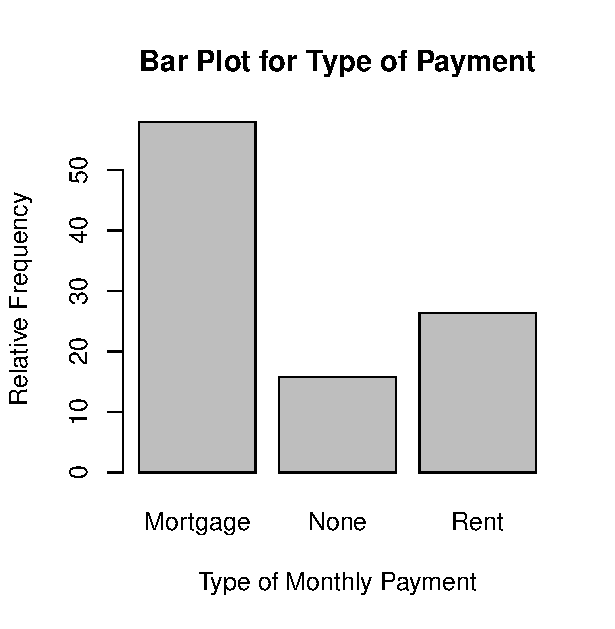
\includegraphics[width=8cm]{figure/LBL2b-1} 

}




\subsection{Pie Chart}

A pie chart gives the same information as a bar chart, except in a circular shape.  We also use pie charts for categorical data.   Some people prefer the look of pie charts over bar charts.  However, studies have shown that people have difficulty comparing relative size of wedges.  Look at the pie chart below.  Is Rent less than half or more than half of Mortgage?



{\centering 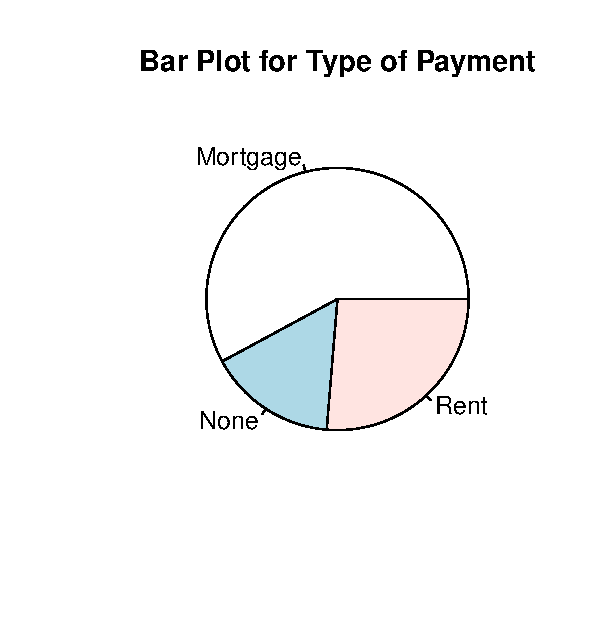
\includegraphics[width=8cm]{figure/LBL2c-1} 

}




\section{Summarizing numerical data}

Consider the variable Monthly Payment in the ACS housing data on page 11.  What do the numbers look like?  How large are they? How variable is the data?  Are there any extreme values? These questions are attempts at getting to know the data.  In this section, we discuss tools for getting to know numerical data better.  We have n = 64 observations available, since 12 households (out of 76) do not have monthly payments.  Here is a list of the monthly payments:

{\small{
880  990  750 1400 1400  560  900  380  910 1200 1200  450 1200 1300  550 340  770  700  700  140  220  650 5200  970  740  500  700 1800  800 1200  1000 1200  200  710 1100  400  370  670  350  510  900  340  440 1500  420    490 2400  500  200  670  760  720  500  280  190 1000  250  700  380  740  850  530  290  230 }}


Now, we sort the observations from smallest to largest:

{\small{
140  190  200  200  220  230  250  280  290  340  340  350  370  380  380  400  420  440  450  490  500  500  500  510  530  550  560  650  670  670  700  700  700  700  710  720  740  740  750  760  770  800  850  880  900   900  910  970  990 1000 1000 1100 1200 1200 1200 1200 1200 1300 1400 1400  1500 1800 2400 5200 }}

The smallest observation is \$140.  The largest is \$5200, which is an \textbf{outlier}.

\fbox{\parbox{14cm}{In data analysis, an \textbf{outlier} is an observation that falls far from the rest of the data.  It may need to be checked for correctness if there is any possiability of clerical error.}}

Can this be a typographical error that we need to correct?  Looking closely at the data, we see it belongs to observation 28, which is a mortgage for a household with \$358,000 annual income.  We infer that it is probably correct, so we leave it alone. The simple act of sorting the data already gives us more information about monthly payment.  For example, we can now see that the typical monthly payment falls around \$700.  We also see the extent to which the \$5200 value is outlying. We now turn to better ways to visualize the \textbf{spread} of this data.

\subsection{Stem-and-Leaf Plot}

Graphs are helpful in summarizing information in the data, especially for large data sets.  Below, we summarize monthly payment in a graph called a stem-and-leaf plot.  The numbers on the left are called stems, while the numbers on the right are called leaves.

There is one leaf for each observation, so there are 63 leaves in all (we left out the \$5200 outlier, for now).  Our smallest observation is \$140.  It is written on the stem `1' as a leaf of `4'.  We can infer that that the stems represent \$100's, and the leaves represent \$10's.  The next largest value \$190 is written on stem `1' as a `9'.   \$200 is written on stem `2' as `0', etc.

\begin{minipage}[ht]{7.5cm}

Stem and Leaf Display of Monthly Payment (stem width \$100)

\begin{tabular}{@{} r|l @{}} \hline
1 & 49 \\
2 & 0023589 \\
3 & 445788 \\
4 & 02459 \\
5 & 0001356 \\
6 & 577 \\
7 & 00001244567 \\
8 & 058 \\
9 & 00179 \\
10& 00 \\
11& 0 \\
12& 00000 \\
13& 0 \\
14& 00 \\
15& 0 \\
16& \\ \hline
\end{tabular}

\end{minipage}
\begin{minipage}[ht]{7.5cm}

Stem-and-Leaf Display of Monthly Payment (stem width=\$200)

\begin{tabular}{@{} r|l @{}} \hline
0 & 49 \\
2 & 0023589445788 \\
4 & 024590001356 \\
6 & 57700001244567 \\
8 & 05800179 \\
10 & 000 \\
12 & 000000 \\
14 & 000 \\
16 &  \\
18& 0 \\
20&  \\
22&  \\
24& 0 \\
26&  \\
28&  \\
30& \\ \hline
\end{tabular}
\end{minipage}

You see why we left out \$1800, \$2400, and \$5200. It would have made the graph extend beyond the page!  We can make the graph more compact by merging stems. The plot below is about half the length because the intervals for each stem are twice as wide.

The stem `8' now contains both `8' and `9', so that the leaves are read as 800, 850, 880, 900, 900, 910, 970, 990.  Which stem-and-leaf plot is better?  The answer depends on the viewers' taste, and is not a matter of right or wrong.  In both cases, we see that monthly payments seem to spread out from around a center of \$700.

Suppose we want to compare mortgage and rent.  Do mortgage payments tend to be greater or less than rent?  We can present stem-and-leaf for mortgage and rent side by side.

\newpage

Stem and Leaf Display of Monthly Payment (stem width \$100)

\begin{minipage}[ht]{3cm}

Mortgage

\begin{tabular}{@{} r|l @{}} \hline
1 & 9 \\
2 & 0039 \\
3 & 478 \\
4 & 245 \\
5 & 00135 \\
6 & 7 \\
7 & 0012457 \\
8 & 05 \\
9 & 007 \\
10& 00 \\
11& 0 \\
12& 0000 \\
13& 0 \\
14& 00 \\
15& 0 \\
16& \\ \hline
\end{tabular}
\end{minipage}
\begin{minipage}[ht]{4cm}

Rent

\begin{tabular}{@{} r|l @{}} \hline
1 & 4 \\
2 & 258 \\
3 & 458 \\
4 & 09 \\
5 & 06 \\
6 & 57 \\
7 & 0046 \\
8 & 8 \\
9 & 1 \\
10&  \\
11&  \\
12& 0 \\
13&  \\
14&  \\
15&  \\
16& \\ \hline
\end{tabular}
\end{minipage}

In general, rent is smaller than mortgages, and less variable.  While mortgages seem centered around \$700, rent is centered around \$500.  Furthermore, mortgages have a longer right tail, with a significant percentage over \$1000.  Plus, remember that we have removed a \$1800 - \$5200 mortgage from these plots.

\subsection{Relative Frequency Table and Histogram}

Earlier in this chapter, we presented a relative frequency table for categorical data.  Relative frequency tables may also be used for numerical data.  A relative frequency table for monthly payment is presented below.  The class width is chosen so as to achieve a moderate number of class intervals.

{\small{
% latex table generated in R 3.4.4 by xtable 1.8-2 package
% Tue May 29 14:29:58 2018
\begin{table}[ht]
\centering
\begin{tabular}{rrr}
  \hline
 & Frequency & Relative Frequency(\%) \\ 
  \hline
0-200 & 2 & 3 \\ 
  200-400 & 13 & 20 \\ 
  400-600 & 12 & 19 \\ 
  600-800 & 14 & 22 \\ 
  800-1000 & 8 & 12 \\ 
  1000-1200 & 3 & 5 \\ 
  1200-1400 & 6 & 9 \\ 
  1400-1600 & 3 & 5 \\ 
  1600-1800 & 1 & 2 \\ 
  2400-2600 & 1 & 2 \\ 
  5200-5400 & 1 & 2 \\ 
   \hline
\end{tabular}
\caption{RF Table of Monthly Payment for ACS Housing Data} 
\end{table}

}}

There are three things to keep in mind when constructing a frequency table. First, decide how many classes (i.e. intervals) you want.  This also determines the \textit{class width}.  Try to have 5 to 15 intervals, depending on how many observations you have. Second, decide where the first interval starts.  Third, decide how to avoid boundary disputes.

The last item requires you to choose a \textbf{boundary convention}.  For instance, the intervals in the frequency table above could have been written as follows:

\begin{tabular}{@{} l @{}} \hline
0-199 \\
200-399 \\
400-599 \\
600-799 \\
etc. \\ \hline
\end{tabular}

This way, it is easier to tell that \$200 belongs to the second interval, not the first.  However, the table looks more complicated, harder to read.  To keep the intervals simple but avoid boundary disputes, include a footnote to the table that describes the boundary convention, i.e. ``Intervals contain the left endpoint but not the right.''  Then, we know that \$200 belongs to the second interval, not the first.  Or, square braces and parenthesis may be used.

\begin{tabular}{@{} l @{}} \hline
$ [0-200)$ \\
$ [200-400)$ \\
$ [400-600)$ \\
$ [600-800)$ \\
 etc. \\ \hline
\end{tabular}

This also means that the class intervals contain the left endpoint but not the right.  Which method do you prefer?

The relative frequency table is a compact numerical way to present how the data is distributed.  If the frequencies are plotted as columns, the resulting plot is called a \textit{histogram}.

The histogram and stem-and-leaf plots look alike, except that the stem-and-leaf plot has columns that go sideways instead of upwards.  Stem-and-leafs are better if you want the data values themselves available from the plot.  However, the histogram can handle large sample sizes easily, and is more flexible in choosing class widths.  For example, you may choose class widths of \$500, as follows: $[0,500), [500,1000), [1000,1500), \dots, [5000,5500)$, which stem plots cannot do.

\subsection{Dot Plot}

For moderately large samples, a \textit{dotplot} diagram is a quick way to see what the data looks like.  We present dotplots of monthly payment for rent and mortgages below.  As we observed using side-by-side stem plots, rent is smaller than mortgages, and less variable.

\begin{figure}[htbp]
   \centering
   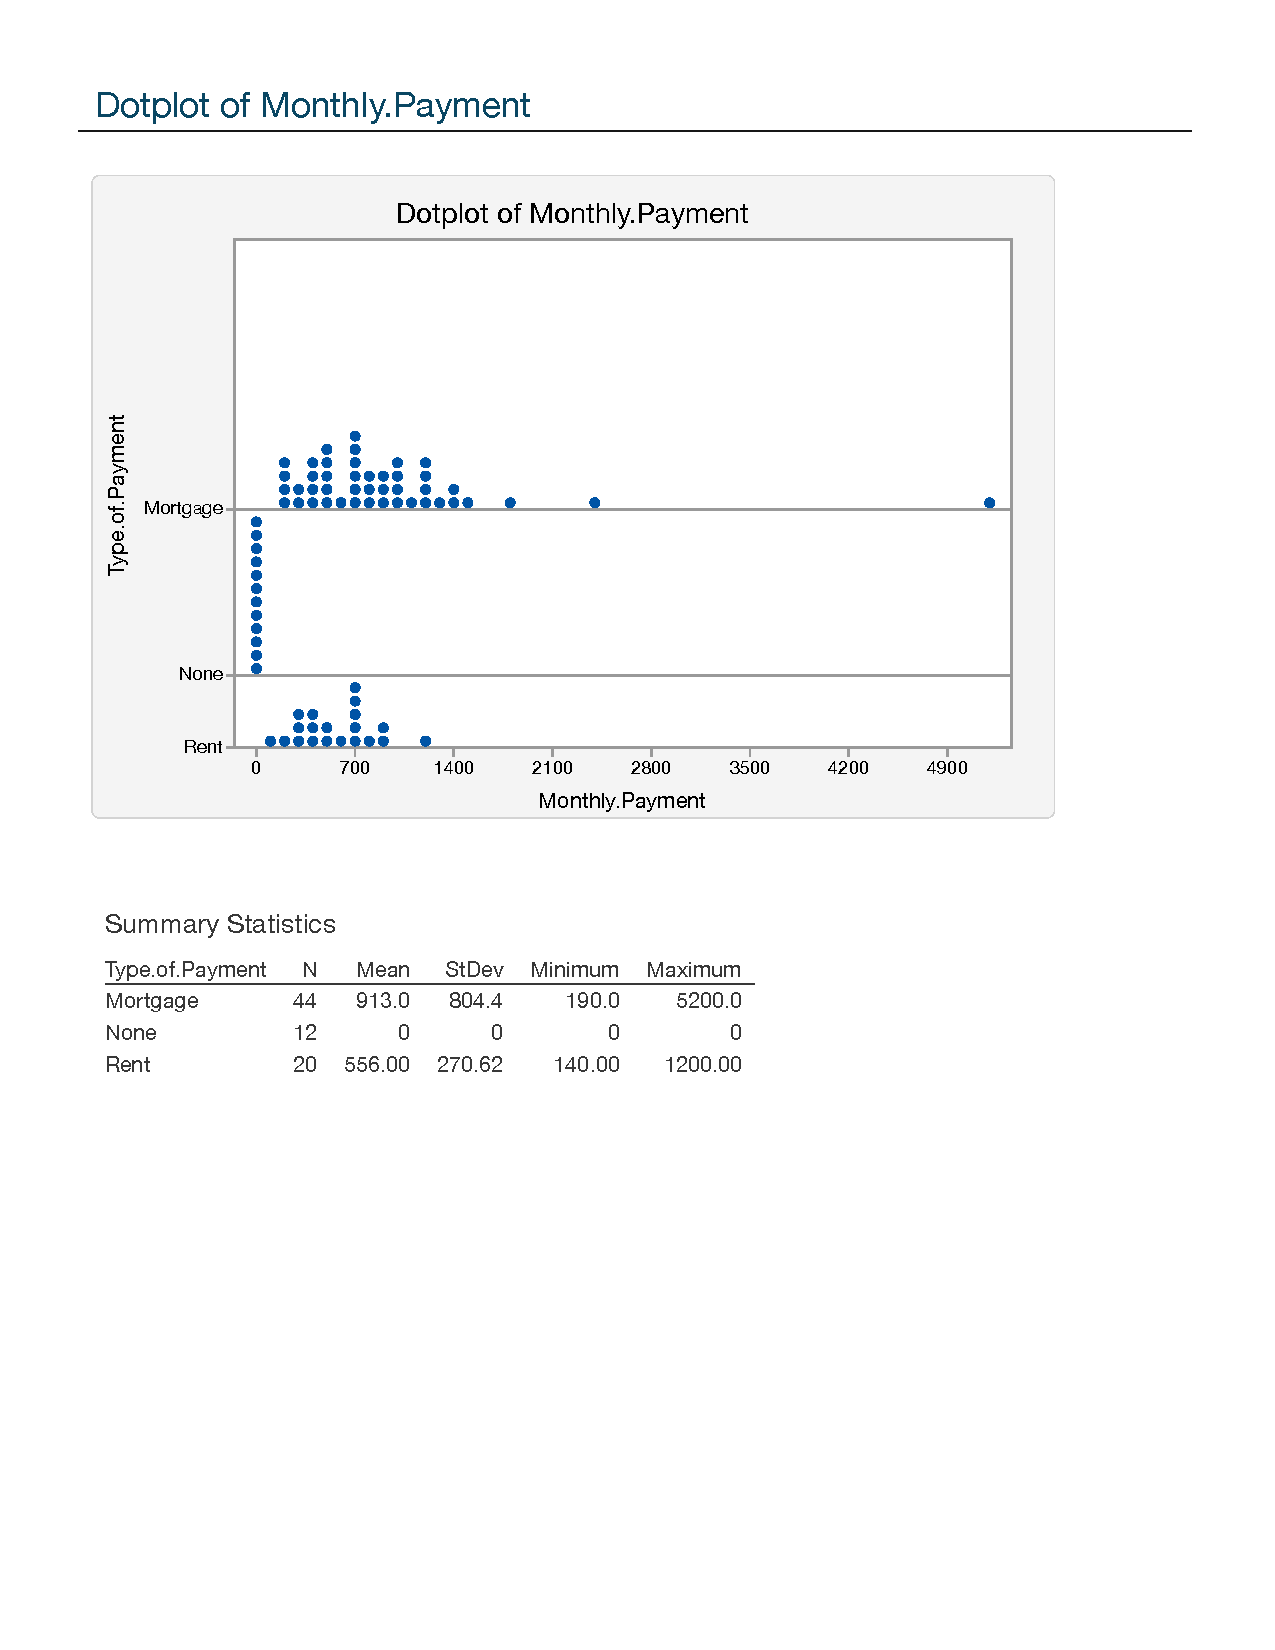
\includegraphics[width=11cm]{chapters/Chapter_2/ext_figure/dotchart.pdf} % requires the graphicx package
   %\caption{example caption}
   %\label{fig:example}
\end{figure}

\subsection{Box-and-Whisker Plot}

A box-and-whisker or boxplot shows useful information about the data including the measures the central tendency and the variability of the distribution.  First, order the data from smallest to largest.  What is the range of the first (or smaller) half of the data?  The smallest quarter of the data?  The next quarter?  The box-and-whisker plot or boxplot is a graphical picture of the distribution of quarters of the data.  Consider once again the monthly payments from the ACS housing data.  We list them here sorted from smallest to largest (minus the \$5200 outlier).
      {\small{
      140  190  200  200  220  230  250  280  290  340  340  350  370  380  380
      400  420  440  450  490  500  500  500  510  530  550  560  650  670  670
      700  700  700  700  710  720  740  740  750  760  770  800  850  880  900
      900  910  970  990 1000 1000 1100 1200 1200 1200 1200 1200 1300 1400 1400
     1500 1800 2400
      }}

There are $n = 63$ observations.  One quarter of the data is 63/4=15.75, or approximately 16 observations.  The boxplot below gives the range of each of the four quarters of the data: the range of the first quarter (i.e. the lowest 16 monthly payments) is given by the left whisker.  The range of the 2nd quarter is the left part of the box, the 3rd quarter the right part of the box, and the range of the last quarter is the right whisker.



{\centering 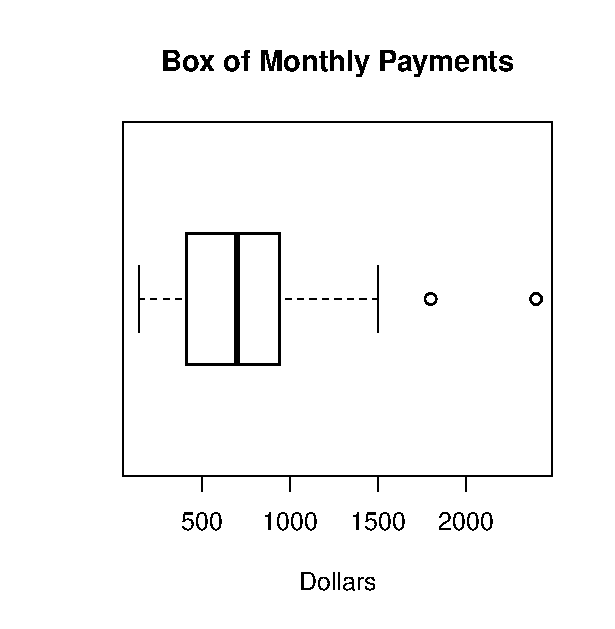
\includegraphics[width=8cm]{figure/LBL2g-1} 

}




More precisely, the vertical lines are drawn at (140, 400, 700, 970, 2400).  Hence, the lowest 16 monthly payments lie within (\$140, \$400).  The next set of 16 observations lie within (\$400, \$700).  The third set lie within (\$700, \$970).  Finally, the last 16 observations lie within (\$970, \$2400).  The five values (140, 400, 700, 970, 2400) that divide the data into quarters and form the fences and whiskers of the boxplot are collectively called the five-number-summary of the data.  They are often denoted as MIN, Q1, MED, Q3, and MAX respectively.

\begin{enumerate}
\item	\textbf{MIN} is called the \textbf{minimum} and is the smallest of the ordered observations.
\item	\textbf{$Q_1$} is the upper boundary of the first quarter and is called the \textbf{first quartile}.
\item	\textbf{MED} is the upper boundary of the second quarter and is called the \textbf{second quartile}.  However, it also divides the data into lower and upper halves and is more often called the median.
\item	\textbf{$Q_3$} is the upper boundary of the third quarter and is called the \textbf{third quartile}.
\item	\textbf{MAX} is the largest of the ordered observations and is called the \textbf{maximum}.
\end{enumerate}

Boxplots are particularly useful for comparing two distributions side-by-side.  Below are boxplots of mortgage and rent drawn parallel to each other on the same scale.  It shows that mortgages tend to be larger than rent, since the median and quartiles are larger.  There is also a very big difference in spread, with mortgage having a long right tail, evidence that mortgages have a higher ceiling than rent.



{\centering 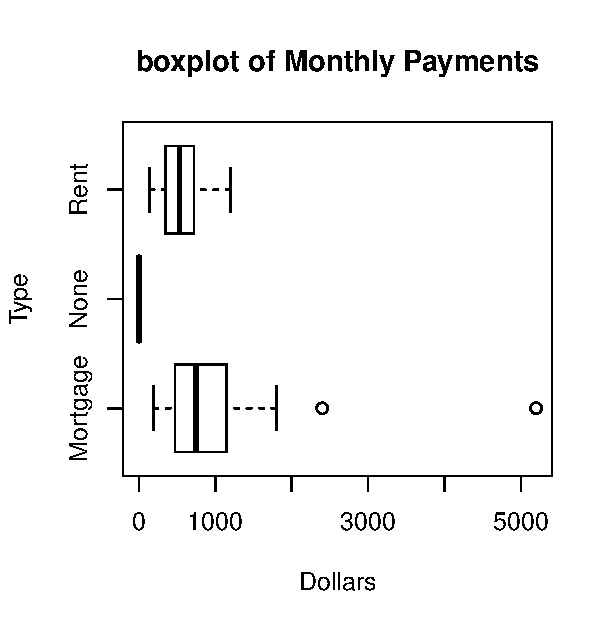
\includegraphics[width=9cm]{figure/LBL2h-1} 

}




Different statistical computing packages have different ways of computing the quartiles, but the differences are minimal.  In this class, we compute the quartiles as follows.  First, arrange the observations from smallest (1st ordered observation) to largest ($n^{th}$ ordered observation).  Then

\fbox{\parbox{9cm}{
$Q_1$ is the .25(n+1)st ordered observation. \newline
MED is the .50(n+1)st ordered observation. \newline
$Q_3$ is the .75(n+1)st ordered observation.
}}

If .25(n+1) is not an integer, take the average of the two adjacent ordered observations.  Similarly, for MED and $Q_3$.  Here again are the $n = 63$ ordered observations of monthly payments.

{\small{
140  190  200  200  220  230  250  280  290  340  340  350  370  380  380
      400  420  440  450  490  500  500  500  510  530  550  560  650  670  670
      700  700  700  700  710  720  740  740  750  760  770  800  850  880  900
      900  910  970  990 1000 1000 1100 1200 1200 1200 1200 1200 1300 1400 1400
     1500 1800 2400
}}


Since .25(63+1)=16, then $Q_1$ is the $16^{th}$ ordered observation.  Hence $Q_1 = 400$.  Similarly, \\ 0.50(63+1)=32 so MED=700.  Finally, .75(63+1)=48, so $Q_3 = 970$.

If $n = 64$, then .25(64+1) = 16.25, so that $Q_1$ would be the average of the $16^{th}$ and $17^{th}$ ordered observations.  Therefore, if we return the \$5200 outlier we removed, then the five-number-summary would be (140, 410, 700, 980, 5200).

\subsection{Symmetry and Skewness}

The shape of the data is often described by its symmetry or non-symmetry (also called skewness).  Here are stem-and-leaf plots for \textit{symmetric}, \textit{right skewed}, and \textit{left-skewed} data.

\vspace{3mm}

\begin{minipage}[ht]{5cm}

Symmetric Data



\begin{tabular}{@{} r|l @{}} \hline
4 & 7 \\
5 & 35 \\
6 & 115 \\
7 & 11112 \\
8 & 467899 \\
9 & 1199 \\
10 & 14 \\
11 & 1 \\ \hline
\end{tabular}
\end{minipage}
\begin{minipage}[ht]{5cm}

Right-Skewed Data



\begin{tabular}{@{} r|l @{}} \hline
4 & 58 \\
5 & 112345569 \\
6 & 2445 \\
7 & 17 \\
8 & \\
9 & 2 \\
10 & 5 \\
11 & 2 \\ \hline
\end{tabular}
\end{minipage}
\begin{minipage}[ht]{5cm}

Left-Skewed Data




\begin{tabular}{@{} r|l} \hline
4 & 0 \\
5 & 5 \\
6 & 2 \\
7 & \\
8 & 17 \\
9 & 2445 \\
10 & 111245569 \\
11 & 58 \\ \hline
\end{tabular}
\end{minipage}

The term `skew' refers to the direction of the longer tail if you flip the stem-and-leaf sideways or draw a histogram.  Here is the histogram of the left-skewed plot below.



{\centering 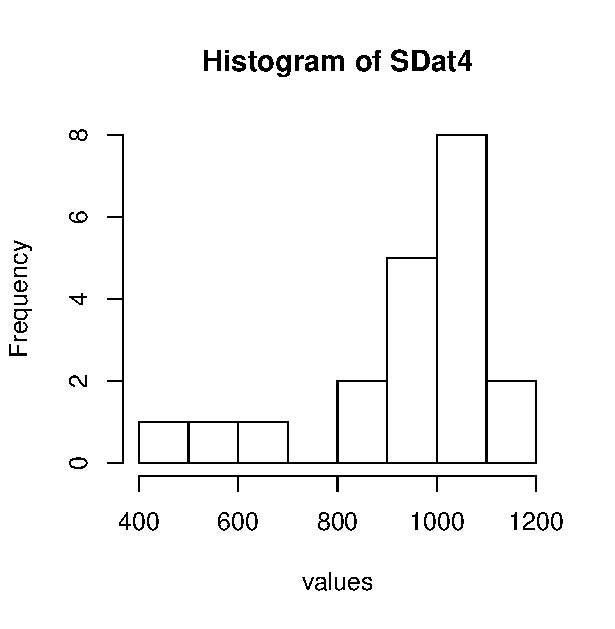
\includegraphics[width=4cm]{figure/LBL2l-1} 

}




The long tail denotes outlying observations or extreme observations.  The left-skewed histogram above contains outlying small observations, while a right-skewed histogram would have outlying large observations.  A left skew also indicates that the smallest quarter of observations will be more spread out. For some further examples of histograms depicting both symmetry and skewness, see below.

\vspace{3mm}

\begin{minipage}[ht]{5cm}



{\centering 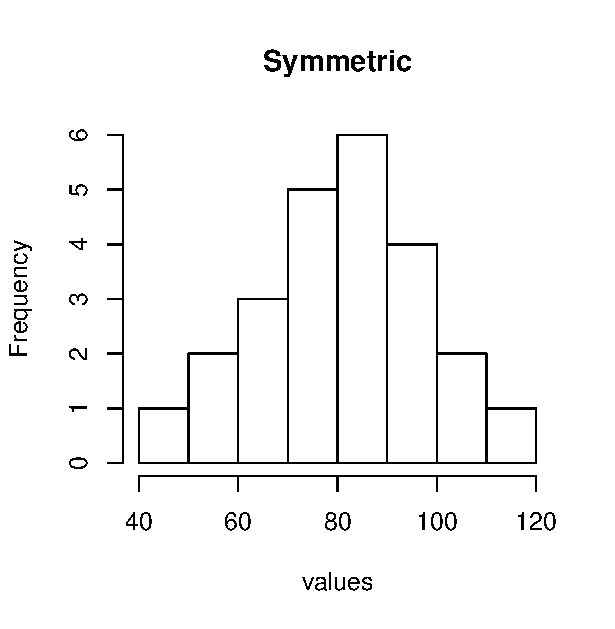
\includegraphics[width=5cm]{figure/LBL2m-1} 

}



\end{minipage}
\begin{minipage}[ht]{5cm}



{\centering 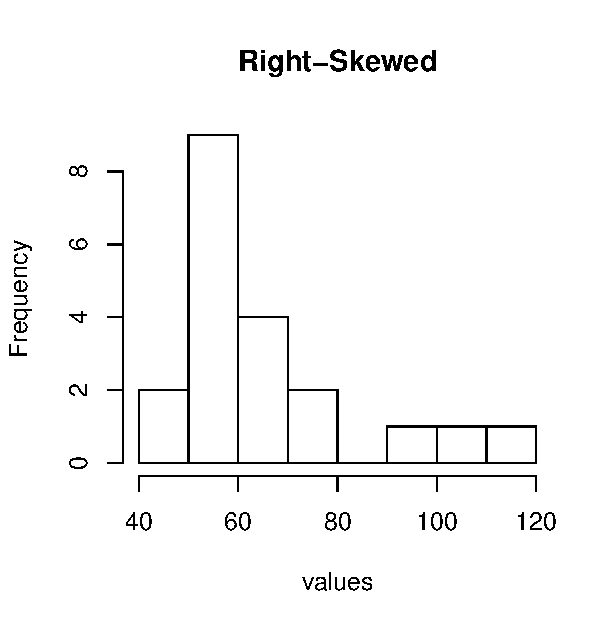
\includegraphics[width=5cm]{figure/LBL2n-1} 

}



\end{minipage}
\begin{minipage}[ht]{5cm}



{\centering 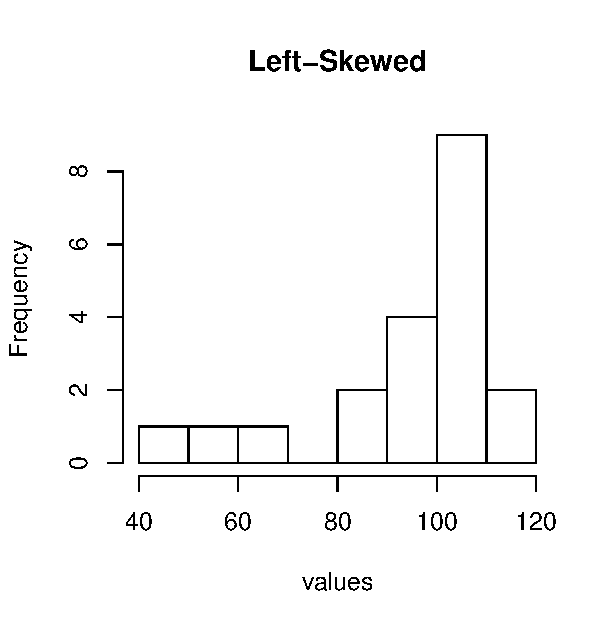
\includegraphics[width=5cm]{figure/LBL2o-1} 

}



\end{minipage}

\newpage

\section{Exercise}

\begin{exercises}    %%%%%%%%%%%%%%%%%%%%%%%%%%%%%%%%%%%%%%%%%%%%

  \begin{exercise}  % 1

Identify the following types of data as numerical or categorical.  If numerical, further classify into interval or ratio.

	  \begin{enumerate}
	  \item The scores on exam one for Stat 1600.
    \item Marital status
    \item Annual income
    \item Social Security Number
    \item Cumulative GPA
    \item Academic level (freshman, sophomore, junior, senior, other)
    \item Quality (poor, fair, good, excellent)
    \item Height (short, average, tall)
    \item Age (years)
    \item Grade $(A, B, C, \dots)$
    \item Color
    \item Rating of eight local plays (poor, fair, good, excellent).
    \item Times required for mechanics to do a tune-up.
  	\end{enumerate}

    % \framebox[5cm][l]{ Answer: }

  \end{exercise}
  \begin{solution}  % 1

    \begin{enumerate}
	  \item The scores on exam one for Stat 1600:  numeric, ratio
    \item Marital status: categorical, nominal
    \item Annual income: numeric, ratio
    \item Social Security Number: categorical, nominal
    \item Cumulative GPA: numeric, interval
    \item Academic level (freshman, sophomore, junior, senior, other): categorical, ordinal
    \item Quality (poor, fair, good, excellent): categorical, ordinal
    \item Height (short, average, tall): categorical, ordinal
    \item Age (years): numeric: ratio
    \item Grade $(A, B, C, \dots)$: categorical, ordinal
    \item Color: categorical, nominal
    \item Rating of eight local plays (poor, fair, good, excellent): categorical, ordinal
    \item Times required for mechanics to do a tune-up: numeric, interval
  	\end{enumerate}
  \end{solution}

  \begin{exercise} % 2


% \begin{minipage}[ht]{7cm}

The 6-year graduation rate for a random sample of 30 colleges and universities
in the U.S. is displayed in the following stem-and-leaf plot.  Note that the stem unit is 10\%, and the leaf unit is 1\%.  For example, the maximum value is 92\%.
% \end{minipage}
% \begin{minipage}[ht]{7cm}

\begin{tabular}{@{} r|l @{}} \hline
2 & \\
3 & 4 \\
4 & 56889 \\
5 & 01112345567889 \\
6 & 0124457 \\
7 & 17 \\
8 & \\
9 & 2 \\ \hline
\end{tabular}
% \end{minipage}

	  \begin{enumerate}
	  \item Obtain the five-number summary.
    \item Obtain a boxplot and histogram for 6-year graduation rate.
    \item In your opinion, which of the three plots (stem-and-leaf, boxplot, histogram) best illustrates the data? Why?
	  \end{enumerate}

 %   \framebox[5cm][l]{ Answer: }
	\end{exercise}
% 	\begin{solution}  % 2
%
%
%   \end{solution}

\begin{exercise}  % 3

The following plots represent five different samples of data. For each, describe the shape.

\begin{figure}[ht]
  \caption{Describe Shapes}

\begin{minipage}[ht]{3cm}

  a)

  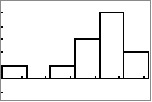
\includegraphics[width=83pt]{chapters/Chapter_2/ext_figure/boxq7.png}
  \end{minipage} \hfill
  \begin{minipage}[ht]{3cm}

  b)

  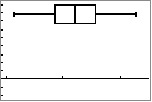
\includegraphics[width=83pt]{chapters/Chapter_2/ext_figure/boxq7b.png}
  \end{minipage} \hfill
  \begin{minipage}[ht]{3cm}

  c)

  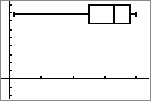
\includegraphics[width=83pt]{chapters/Chapter_2/ext_figure/boxq7c.png}
  \end{minipage} \hfill
  \begin{minipage}[ht]{3cm}

  d)

    \begin{tabular}{@{} r|l @{}} \hline
  4 & 58 \\
  5 & 011245569 \\
  6 & 2445 \\
  7 & 17 \\
  8 &  \\
  9 & 2 \\
  10 & 5 \\
  11 & 0
    \end{tabular}
  \end{minipage} \hfill
  \begin{minipage}[ht]{3cm}
  e)

  \begin{tabular}{@{} r | l @{}} \hline
  0 & 4 \\
  1 & 889 \\
  2 & 11467 \\
  3 & 457 \\
  4 & 7
  \end{tabular}
  \end{minipage}

\end{figure}
\end{exercise}
\begin{solution}  % 3

2.5-7.1: Left-skewed

2.5-7.2: Symmetric

2.5-7.3: Left-skewed

2.5-7.4: Right-skewed

2.5-7.5: Symmetric

\end{solution}


  \begin{exercise} % 4

A manager of a car rental company took a random sample of 100 business days over the last fiscal year and recorded the number of cars rented per day.  The frequency distribution for the data is given below.

\begin{tabular}{@{} lcc @{}} \hline
Interval  &  Frequency &	Relative Frequency \\
$(20, 25]$ 	&      4 \\
$(25, 30]$ 	&    11  \\
$(30, 35]$ 	&    23 \\
$(35, 40]$ 	&    31 \\
$(40, 45]$ 	&    15 \\
$(45, 50]$ 	&    10 \\
$(50, 55]$ 	&      6 \\ \hline
\end{tabular}

\begin{enumerate}
\item Fill in the Relative Frequencies above.
\item	Draw a histogram by hand, with either the frequencies or relative frequencies as the vertical axis.
\item	What interval does the median number of car rentals per day fall into?
\item What percentage of business days had 30 or less car rentals?
\item	How many business days had more than 45 car rentals?
\end{enumerate}

   % \framebox[5cm][l]{ Answer: }

	\end{exercise}
	\begin{solution}  % 4


Compute relative frequencies:

\begin{tabular}{@{} lcc @{}} \hline
Interval  &  Frequency &	Relative Frequency \\
$(20, 25]$ 	&     4 & 4  \\
$(25, 30]$ 	&    11 & 11 \\
$(30, 35]$ 	&    23 & 23 \\
$(35, 40]$ 	&    31 & 31 \\
$(40, 45]$ 	&    15 & 15 \\
$(45, 50]$ 	&    10 & 10 \\
$(50, 55]$ 	&     6 & 6 \\ \hline
\end{tabular}


	\end{solution}

\end{exercises}



%!Rnw root = ../../Master.Rnw

\chapter{Location and Spread}
\label{chap:ch3}

\section{Objective}

After completing this part, students should be able to:

\fbox{\parbox{14cm}{
\begin{itemize}
\item Explain the concept of measures of central tendency and interpret the
information they provide.
\item Calculate, describe and compare the three most commonly used measures of central tendency: means, medians, and modes.
\item Understand other measures of central tendency
\item Select appropriate measure of central tendency based on the
level of measurement and characteristics of the data (distribution).

\item Explain the concept of measures of dispersion and the information they convey.
\item Compute and explain the following:
	\begin{itemize}
	\item The range ({\textbf{R}}).
	\item The interquartile range ({\textbf{IQR}})
	\item The sample variance (denoted as {\textbf{$s^2$}}).
	\item The population variance  (denoted as {\textbf{$\sigma^2$}}).
	\item The sample standard deviation  (denoted as {\textbf{$s$}}).
	\item The population standard deviation  (denoted as {\textbf{$\sigma$}}).
	\end{itemize}
\item Select the  measure of dispersion appropriate for our current problem.
\end{itemize}
}}


\section{Estimates of Center}

Suppose that a random sample of two-bedroom apartments in the Kalamazoo area yields the following data on monthly rent:

\$635, \$525, \$500, \$800, \$650, \$750, \$555, \$500, \$670, \$675

How much would you say is the average rental for two-bedroom apartments in Kalamazoo?  In this chapter, we will discuss the sample average and several alternatives to the average when estimating `average value' in a population.

\subsection{The Sample Mean}

The sample mean is the statistical term for `average of the sample.'  For the example above, the sample mean (denoted $\bar{X}$) is: The sample mean is the statistical term for `average of the sample.'  For the example above, the sample mean (denoted $\bar{X}$) is:

$$ \bar{X} = \frac{635+525+500+800+650+750+555+500+670+675}{10} = \$626 $$

so that the average rent in Kalamazoo may be estimated as \$626.  Note that this is an \textit{estimate} based on a \textit{sample}.  Therefore, it is subject to \textit{sampling error}.   Sampling error simply means that due to luck of the draw, the sample average likely missed the true population average.  More precisely, the two-word term `sampling error' refers to $| \bar{X} = \mu |$,  the distance by which the \textit{sample} average $\bar{X}$  misses the population average  $\mu$.

Advantages of the mean:

\begin{itemize}
\item It is easy to understand and simple calculate.
\item It is based on all the values.
\item It is not based on the position in the series.
\end{itemize}

Disadvantage of the mean:

\begin{itemize}
\item It is always affected by small and large values.
\end{itemize}

\subsection{The Sample Median}

There are alternative ways to estimate average rent.  We can compute the sample
median, instead of the sample mean.  We have discussed the sample median (denoted MED) earlier in Chapter 1.  It is computed as follows.

\begin{enumerate}
\item Let $n$ represent the total number of observations.
\item Order the $n$ observations from smallest to largest.
\item Then calculate $0.50(n + 1)$.
\item If $0.50(n + 1)$. is an integer, then MED is the $0.50(n + 1)st$ ordered observation.
\item If $0.50(n + 1)$ is not an integer, then MED is the average of the two adjacent ordered observations.
\item There are $n = 10$ observations in our rental data.  We first order them from smallest to largest.
\end{enumerate}

$$ 500, 500, 525, 555, 635, 650, 670, 675, 750, 800 $$

Now, $0.50(n + 1) = 0.50(10 + 1) = 5.5$.  Since this is not an integer, we average the $5^{th}$ and $6^{th}$ largest observations:

$$MED = \frac{(635 + 650)}{2} = \$642.50$$

The advantage of the median is that it is more robust than the mean, i.e., the median is not as affected by extreme values (outliers).

\subsection{The Trimmed Mean}

Since the mean uses all observations in the calculation, it can be strongly affected by outlying small and large values.  What happens to the mean when the smallest value \$500 is replaced by \$400?  It will become smaller.  What happens to the median?  It remains unchanged.

The trimmed mean is a compromise estimator that looks a lot like a mean but is less sensitive to extreme values.  The 10\%-trimmed mean removes the lowest 10\% and highest 10\% of the data, then takes the sample mean of the remaining data.  In the rental example, 10\% of the data is one observation. We remove the lowest
observation (\$500) and the largest observation (\$800), and take the mean of the remaining 8 observations:

$$\bar{X} = \frac{635+525+650+750+555+500+670+675}{10} = \$620$$

What if 10\% of the data is not an integer?  For example, if $n = 23$, then 10\% of n is 2.3.  Since we cannot remove 2.3 observations, we will remove 3 observations from each end (to ensure at least 10\% protection) and take the average of the middle 17 observations.

\subsection{The Median of Pairwise Averages}

The median of pairwise averages is another compromise between the mean and median.  As the name implies, we replace the observations by pairwise averages, then take the median of those.  Here again are the 10 ordered observations:

$$ 500, 500, 525, 555, 635, 650, 670, 675, 750, 800 $$

The first observation (\$500) is paired with all 10 observations (including itself).  The second observation (also \$500) has already been paired with the first observation, so it paired with only 9 observations (including itself).  The third observation (\$525) has already been paired with the first two observations, so it is paired with only 8 observations (including itself).  Proceeding in this pattern, we get the following pairwise averages:

Picture of

There will be 55 pairwise averages in all.  Notice that the sample size, $n$, went from 10 observations to 55 observations after we do this.  We now need to figure the median and remember, the MED is the $0.50(n + 1)st$ ordered observation.  So we need to use 55 now as our $n$.  This gives us a value of 28.  We need order the pairwise averages we have calculated above and the median will be the 28th observation.  The median of these averages is thus \$625.

\section{Estimate of Spread (or Uncertainty or Variation)}

Recall the data on monthly rent of two bedroom apartments in the Kalamazoo area:

$$ 500, 500, 525, 555, 635, 650, 670, 675, 750, 800 $$

If a future student asked you ``What do you think a two-bedroom apartment would cost me in rent?'', how would you reply? Knowing that the data averages \$626, you might say something like ``Around \$626, give or take $\dots$(?).''   This second number, the give or take, is important because it says how much uncertainty there is in your guess.  In other words, the student's rental will probably miss \$626, but by how much?  For a second example, if you were going to San Francisco for a couple of days in August, and you want to know what clothes to bring, it is not enough to know that the average temperature is 68 degrees.  If it was 68 degrees, give or take 15 degrees, then you will need a sweater.  If it is 68 degrees, give or take 30 degrees, you might need a winter coat.

Variation presents itself everywhere.  Consider weight loss.  The 77 subjects in the Atkins group lost an average of 10.5 pounds give or take 15 pounds.  Compare this to an average of 3.5 pounds for the Zone diet give or take 14 pounds. How about in bowling?  In his first 7 games in a tournament in Indiana, Walter Ray Williams Jr. averaged 228, give or take 34.   Notice how the give or take number seems to complete the description.

In this chapter, we will discuss the sample standard deviation, which is typically used as the ‘give or take’ number to describe spread in a group of numbers.

\subsection{The Sample Standard Deviation}

The standard deviation (or SD) for the monthly rent data is computed using a series of steps.  Notice in the last row we have the average, the sum of the deviations from the mean, which will always be 0, and the Sum of Squares (SS) which is the sum of the squared deviations.


% latex table generated in R 3.4.4 by xtable 1.8-2 package
% Tue May 29 14:29:58 2018
\begin{table}[ht]
\centering
\begin{tabular}{rrrr}
  \hline
 & Rent & Deviations & SS \\ 
  \hline
1 & 635 & 9 & 81 \\ 
  2 & 525 & -101 & 10201 \\ 
  3 & 500 & -126 & 15876 \\ 
  4 & 800 & 174 & 30276 \\ 
  5 & 650 & 24 & 576 \\ 
  6 & 750 & 124 & 15376 \\ 
  7 & 555 & -71 & 5041 \\ 
  8 & 500 & -126 & 15876 \\ 
  9 & 670 & 44 & 1936 \\ 
  10 & 675 & 49 & 2401 \\ 
  Sum & 6260 & 0 & 97640 \\ 
   \hline
\end{tabular}
\end{table}


$$ SD = \sqrt{ \frac{ SS}{n - 1}} = \sqrt{ \frac{ \ensuremath{9.764\times 10^{4}}}{9}} \approx 104.2 $$

It is helpful to get a feel for the numbers in the second column.  The first value 9 says that `635 is 9 above average'.  The next number -101 says that `525 is 101 below average.'  Ignoring signs, the numbers in the second column represent the `give or take' from the average.  To get the actual SD, we take the Sum of Squares and divide by $(n - 1)$, and last of all take the square root of that answer.  This gives us a final SD of 104.158.  We say that monthly rent averages \$626, give or take \$104.

Look at the second column again.  Ignoring signs, these are the distances from the average.  Which rental is closest to the average? The answer is \$635, which missed by 9. Which rental is farthest from the average?  \$800, which missed by 174.
What is the average `size of the miss?'  This should be somewhere between the smallest and largest, right?  This is how you interpret the SD: ``On the average, the monthly rentals miss the mean by \$104.''

Taken together, the mean and SD allow comparison of both relative size and spread of two groups of numbers.  In the professional bowling tournament in Indiana that he won in November of 2008, here are Walter Ray Williams Jr.'s first seven  games and last seven games (including the final):

% Requires the booktabs if the memoir class is not being used
\begin{table}[htbp]
   \centering
   %\topcaption{Table captions are better up top} % requires the topcapt package

   \begin{tabular}{@{} | lccc | @{}} \hline
      Games &  & Mean & SD \\ \hline
      First seven & 163,231,224,238,279,239,226 & 228.6 & 34.3 \\
      Last seven  & 246,244,247,248,237,258,246 & 246.6 & 6.2 \\ \hline
   \end{tabular}

   % \caption{Remember, \emph{never} use vertical lines in tables.}
   % \label{tab:booktabs}
\end{table}

What do the mean and SD tell us?  He averaged higher in the end but was also more consistent with a give-or-take of only 6 points!  His earlier games had bigger swings: from a low of 163 to a high of 279, resulting in a SD of 34.

\subsection{Effect of Multiplication and Addition by a Constant}

Recall that monthly rent for apartments average \$626 with an SD of \$104.  If the student plans to get a roommate and pay only half the rent, how much does he expect to pay?  If you are thinking of halving both numbers, i.e. \$313 give or take \$52, this is correct.

\begin{center}
Original rent: $ 626 \pm 104 $ \hspace{2cm}	Half the rent: $ 313 \pm 52 $
\end{center}

Now suppose that the student does not plan to get a roommate, but his parents have agreed to contribute \$100 to rent each month.  How much does the student expect to pay after the \$100 subsidy? If you are thinking of subtracting \$100 from both numbers, i.e. \$426 give or take \$4, this is wrong.  The SD should remain the same, i.e.,

\begin{center}
Original rent: $ 626 \pm 104 $ \hspace{2cm} Subsidized rent: $ 526 \pm 104 $
\end{center}
If you are not convinced, consider the data itself on the following table.

% latex table generated in R 3.4.4 by xtable 1.8-2 package
% Tue May 29 14:29:58 2018
\begin{table}[ht]
\centering
\begin{tabular}{rrrr}
  \hline
 & Rent & Deviations & SS \\ 
  \hline
1 & 317.5 & 4.5 & 20.2 \\ 
  2 & 262.5 & -50.5 & 2550.2 \\ 
  3 & 250.0 & -63.0 & 3969.0 \\ 
  4 & 400.0 & 87.0 & 7569.0 \\ 
  5 & 325.0 & 12.0 & 144.0 \\ 
  6 & 375.0 & 62.0 & 3844.0 \\ 
  7 & 277.5 & -35.5 & 1260.2 \\ 
  8 & 250.0 & -63.0 & 3969.0 \\ 
  9 & 335.0 & 22.0 & 484.0 \\ 
  10 & 337.5 & 24.5 & 600.2 \\ 
  Sum & 3130.0 & 0.0 & 24410.0 \\ 
   \hline
\end{tabular}
\caption{Calculating the SD when rent is halved} 
\end{table}


$$ SD = \sqrt{ \frac{ SS}{n - 1}} = \sqrt{ \frac{ \ensuremath{2.441\times 10^{4}}}{9}} \approx 52.08 $$

\fbox{\parbox{14cm}{In general, when the data is \textbf{multiplied or divided by a positive constant}, the \textbf{same thing happens} to both the average and the SD}}

% latex table generated in R 3.4.4 by xtable 1.8-2 package
% Tue May 29 14:29:58 2018
\begin{table}[ht]
\centering
\begin{tabular}{rrrr}
  \hline
 & Rent & Deviations & SS \\ 
  \hline
1 & 535.0 & 9.0 & 81.0 \\ 
  2 & 425.0 & -101.0 & 10201.0 \\ 
  3 & 400.0 & -126.0 & 15876.0 \\ 
  4 & 700.0 & 174.0 & 30276.0 \\ 
  5 & 550.0 & 24.0 & 576.0 \\ 
  6 & 650.0 & 124.0 & 15376.0 \\ 
  7 & 455.0 & -71.0 & 5041.0 \\ 
  8 & 400.0 & -126.0 & 15876.0 \\ 
  9 & 570.0 & 44.0 & 1936.0 \\ 
  10 & 575.0 & 49.0 & 2401.0 \\ 
  Sum & 5260.0 & 0.0 & 97640.0 \\ 
   \hline
\end{tabular}
\caption{Calculating the SD when rent is reduced by 100 dollars} 
\end{table}


$$ SD = \sqrt{ \frac{ SS}{n - 1}} = \sqrt{ \frac{ \ensuremath{9.764\times 10^{4}}}{9}} \approx 104.16 $$

\fbox{\parbox{14cm}{ In general, when a \textbf{constant is added or subtracted} to the data, the same thing happens to both the average,  but the \textbf{SD remains unchanged.}}}

\newpage
\twocolumn
\section{Exercises}
\begin{exercises}

  \begin{exercise} % 1

The carbon monoxide measures (in mgs) are given on 25 brands of \\ cigarettes.

13.6    16.6    23.5    10.2     5.4     15.0     9.0    12.3    16.3   15.4
13.0    14.4    10.0    10.2     9.5      1.5    18.5    12.6    17.5    4.9
15.9     8.5    10.6    13.9    14.9

Calculate the

\begin{enumerate}
\item Mean
\item median
\item 10\% trimmed-mean
\item standard deviation
\item mean and standard deviation (in grams)
\end{enumerate}

	\end{exercise}
	\begin{solution}  % 1


	Compute the mean, median, $\dots$ for carbon monoxide:
  \begin{enumerate}
  \item mean = 12.5
  \item median = 13.0
  \item Trimmed mean = 12.7
  \item SD = 4.74
  \item Mean = 0.0125 and standard deviation 0.00474 (in grams)
	\end{solution}

  \begin{exercise} % 2

  Calculate the median of \\ pairwise average for the first 6 observations which are listed below:

13.6    16.6    23.5    10.2     5.4     15.0

 	\end{exercise}
 	% \begin{solution}  % 2
 	%
 	%
 	% The third value must be 22 so that the average is 20 for all three quizzes.
 	% \end{solution}

  \begin{exercise} % 3

  Daily high temperature for a given day are provided for the past 10 years

\begin{tabular}{@{} ccccc @{}} \hline
2007&2008&2009&2010&2011 \\
59&50&49&13&41 \\ \hline
2012&2013&2014&2015&2016 \\
46&51&53&58&47 \\ \hline
\end{tabular}

Find the following statistics for \\ temperature:

\begin{enumerate}
\item Range
\item Mean
\item Median
\item Mode
\item Remove the temperature of the year \\ 2010 from the data set and re-calculate the Mean and compare it with part c? Is the mean closer to the median and why?
\end{enumerate}


   \end{exercise}
   \begin{solution} % 3



\begin{enumerate}
\item The range is from 13 to 59
\item the mean is 46.7
\item The median is 49.5
\item There is no mode since there are no duplicates.
\item Removing the smallest value changes the mean to 50.4.  The new value is closer to median because 13 is an outlier.
\end{enumerate}
  \end{solution}

   \begin{exercise} % 4

Joshua has been working on \\ programming  and updating a Website for his \\ company for the past 12 months. The following numbers represent the number of hours Joshua  has worked on this Website for each of the past 12 months:

24, 25, 31, 40, 48, 40, 36, 50, 38, 35 ,42, 112

\begin{enumerate}
\item Calculate the mean
\item Calculate the median
\item Decide if its symmetric, skewed to the right or to the left
\item Decide which measure of center provides the most relevant information about the distribution? Why?
\end{enumerate}

\end{exercise}
\begin{solution}


\begin{enumerate}
\item the mean is 43.4166667
\item the median is 39
\item Decide if its symmetric, skewed to the right or to the left: the data is right skewed
\item Decide which measure of center provides the most relevant information about the distribution? Why?  The median is the most relevant information because the data is right skewed.
\end{enumerate}

\end{solution}

\end{exercises}

\onecolumn


%!Rnw root = ../../Master.Rnw

\chapter{Threats to Valid Comparisons}
\label{chap:ch4}

\section{Objective}

After completing this part, students should be able to:

\fbox{\parbox{14cm}{

 \begin{itemize}
 \item Explain the logic of hypothesis testing
 \item Define and describe the elements of hypothesis testing
 	\begin{enumerate}
 	\item Verify assumptions
 	\item State null and alternative Hypotheses \index{hypotheses}
 	\item Identify the appropriate critical values  and rejection region
 	\item Perform the appropriate test based on data in one-sample (both one and two-tailed tests). \index{two-tailed}
 	\item Identify the appropriate conclusion based on the test and be able to explain Type I and Type II errors and how they relate to the selection of the significance of the trial   $\alpha$ and $\beta$ risks).
 	\item Comment on the effect size.
 	\end{enumerate}
 \end{itemize}
 }}

\section{Hidden Confounder}  \index{confounds}

In 1992, a research study “Lower extremity fractures in motor vehicle collisions:
Influence of direction of impact and seatbelt use” by Dischinger, P., Cushing, B. and Kerns, T. was published in the 36th Proceedings of the Association for the Advancement of Automotive Medicine.  It involved data analysis of the trauma-center population in Maryland.  Some of the conclusions were:

\begin{enumerate}
   \item there was a higher incidence of lower extremity injury in frontal collisions,
   \item seatbelt use was not effective in preventing lower extremity fractures, and
   \item there was a higher incidence of lower extremity fracture among women.
\end{enumerate}

The conclusion (3) is interesting.  It begs the follow-up question: ``Why do women have higher rates of leg fractures?''  Is it because they drive faster, or apply brakes more slowly, or have weaker bones?  It turns out that these are false questions -- they presume that gender is the variable that causes higher leg fractures.

An explanation was proposed in a follow-up study with the same lead author: ``Lower extremity fractures in motor vehicle collisions: The role of driver gender and height'' by Dischinger, P.C., Kerns, T.J., Kufera, J.A. Accident Analysis \& Prevention Volume 27, Issue 4, August 1995.

\begin{quotation}
Abstract: In a previous study it was noted that there was a higher incidence of lower-extremity fractures among women drivers. Analyses were based on a linkage between trauma registry and police crash report data. The present study addresses the issue of whether the differences noted are attributed to driver gender or are merely a reflection of differences in driver height. An inverse association was noted between driver height and the incidence of lower-extremity fractures. Those shorter than average (5'7'') for this population had a 64\% increase in lower-extremity fracture, which can be mainly attributed to ankle/tarsal injuries. Thus, the incidence of these injuries appears to be a function of driver height, with an increase among shorter drivers, most of whom are women.
\end{quotation}

It turns out that height was the culprit, but it initially looked like gender because height and gender have a strong link.  The following \textit{pathway graph} describes the true relationship:

\begin{eqnarray*}
\texttt{Height} & \Rightarrow & \texttt{Leg Fracture} \\
\updownarrow &  & \\
\texttt{Gender} & &
\end{eqnarray*}

But the association between height and gender led us to believe the wrong relationship

$$ \texttt{Gender} \Rightarrow  \texttt{Leg Fracture} $$

The symbol $\Rightarrow$ represents ``cause-and-effect'' while $\updownarrow$      represents ``association.''

In this situation, leg fracture rate is the outcome variable gender is the probable cause.  The hidden variable height is called a \textbf{confounder}, or a confounding variable.

\fbox{\parbox{14cm}{
\textbf{Confounding Variable:} \\
A confounder or confounding variable is a third variable that is associated with both the probable cause and the outcome.  It can lead us to a wrong conclusion about the cause-and-effect relsationship.
}}

\subsection{Apples and Oranges}

Now, why do hidden confounders belong in a chapter on threats to valid comparisons? Because they are one of the biggest sources of (often unknowingly) invalid comparisons.  It seemed fair to compare leg fracture rates of men and women, didn't it?  What's wrong with that?  Unfortunately, with respect to leg fracture rates, it was a case of comparing apples to oranges -- women as a group are shorter than men!  Of course, in the 1992 study, the investigators did not know that height would make a difference.  Women also tend to weigh less, smoke less, drink less, have longer hair, and wear higher heels.  Which of these would make a difference, i.e. be potential confounders?

Confounders are a big problem in comparison studies.  Some confounders may remain hidden, but it is critical that the researcher identify and control for potential confounders as much as possible.  Does smoking cause lung cancer?  When comparing smokers to nonsmokers, it is easy to show that smokers have higher lung cancer rates.  But as a group, they exercise less than nonsmokers.  They drink more coffee than nonsmokers.  Can the exercise or the coffee or the combination be the culprit?  Furthermore, smokers tend to be male, older, and drive in the winter with their car windows open.  There are plenty of confounding variables even in this comparison.

\subsection{In the news}

The STATS website (http://www.stats.org/) is dedicated to correcting ``scientific
misinformation in the media and in public policy resulting from bad science,
politics, or a simple lack of information or knowledge.''  The following is an excerpt from an article written by Rebecca Goldin and Jing Peng in August 2010.  What is the confounding variable?  The probable cause? The outcome variable?

\begin{quotation}
\textbf{If you take Viagra, will you get an STD?} \\
Rebecca Goldin Ph.D. and Jing Peng, August 2, 2010

To judge from recent headlines, the risk seems clear: ``Sex Diseases Tripled in Men 40 or Older Taking Viagra, Cialis, Study Says'' reports Bloomberg; ``Older Viagra Users More Likely to Get STDs'' says the Chicago Sun Times, presumably comparing older Viagra users with older non-Viagra users.  And Health Day was even more explicit, saying ``Drugs Like Viagra Linked to Higher Rates of STDs.''  The immediate logic behind the claim seems persuasively obvious: if men who take Viagra are having more sex, then they have surely increased their risk of catching a sexually transmitted disease (STD). But is this really the case?

The study compared men who took erectile dysfunction (ED) drugs with those who did not.  Researchers found that ED drugs such as Viagra are linked to higher rates of STDs among older men, but not older women, especially after the introduction of Viagra in 1998.  A study published in the July 6 issue of the Annals of Internal Medicine was the first to examine the relationship between ED drugs and STDs. But its findings turn out to be far different than media accounts would have you believe.

The main problem in the coverage is the direct suggestion that taking Viagra is associated with STDs, as opposed to being the sort of person who takes Viagra.

This is a critical distinction. To see what it means, let's go backward in time and
compare STD rates among people who plan to take Viagra but haven't and people who are not planning on taking Viagra. This clever comparison is what the authors of the research article did; they combed medical records for people who filled prescriptions for ED drugs, and compared STD rates for these people prior to filling their prescription to the STD rates of people who did not subsequently fill a prescription for Viagra.  It turns out that the rate of STDs is higher among people who intend to take it.  In other words, the drug is absent, but those people who will take Viagra within a year are already at higher risk of STDs.

In fact, compared to those who don't take ED drugs, those who plan to take Viagra had a slightly higher rate for STDs, an odds ratio (OR) of 2.80; 95\% confidence interval CI, 2.10 to 3.75, than those who actually take it (OR) 2.65, CI, 1.84 to 3.81, though the difference was not significant. This means that the drug had no discernable effect on STD rates for this group of men.
\end{quotation}

The paper goes on with detailed analysis, but the main point has been stated.  To summarize the conclusions of the study:

\begin{enumerate}
	\item Taking ED drugs do not increase the rate of STD's
	\item The type of people who take ED drugs are different from people who do not.

	\begin{eqnarray*}
\texttt{Person type} & \Rightarrow & \texttt{STD} \\
\updownarrow &  & \\
\texttt{ED drugs} & &
\end{eqnarray*}

instead of the (admittedly more sensational) relationship implied by the headlines.

\end{enumerate}


% \pagebreak

\section{Key Words}

% \colorbox{lgray}{\parbox{14cm}{
%
% \begin{minipage}[ht]{6cm}
%
% \begin{itemize}
% \item $\alpha$ level
% \item Critical region
% \item Five-step model
% \item Hypotheses testing
% \item One-tailed test
% \item Research hypothesis
% \item Student's t-distribution
% \item $t$-critical
% \end{itemize}
% \end{minipage} \hfill
% \begin{minipage}[ht]{6cm}
%
% \begin{itemize}
% \item $t$-obtained
% \item Test statistic
% \item Two-tailed test
% \item Type I error (alpha error)
% \item Type II error (beta error)
% \item $Z$-critical
% \item $Z$-obtained
% \end{itemize}
% \end{minipage}
%
% }}

% \newpage
\twocolumn
\section{Exercises}

\begin{exercises}

% \begin{exercise}  % dummy
%
%   what is x + y, when x = 5 and y = 5
%
% \end{exercise}
  \begin{exercise} % 1

Study says, ``Slightly overweight people live longer than thin people.''

\begin{enumerate}
  \item The headline implies cause-and-effect, \\ not just association, i.e. ``if you are thin, you should try to gain weight.''  When comparing life span of slightly over- \\ weight and thin people, what possible confounders can you think of?
  \item Using one confounder from your \\ answer(s) in (1), draw a pathway graph depicting the possible relationship between confounder, possible cause and \\ outcome.
\end{enumerate}

	\end{exercise}
	\begin{solution}  % 1

	  $H_0: \mu = 6.2$ vs. $H_A: \mu \neq 6.2$
	\end{solution}

  \begin{exercise} % 2

A study that appeared in the American journal of cardiology (March 15, 2003) found out that ``heart attack survivors who owned a dog generally had better heart function post-heart attack than those who did not own a dog.''

\begin{enumerate}
  \item Does a dog help a heart heal faster?  \\ What possible confounders can you \\ think of?
  \item Using one confounder from your \\ answer(s) in (1), draw a pathway graph depicting the possible relationship between confounder, possible cause and \\ outcome.
\end{enumerate}

	\end{exercise}
	% \begin{solution}  % 2
	%
	%     $SE = \frac{0.7}{\sqrt{25}} = 0.14$  \\
	%     $t = \frac{(5.9 - 6.2)}{0.14} = -2.14$
	%
	% \end{solution}

  \begin{exercise} % 3

Study says, ``People who \\ consider themselves depressed eat more \\ chocolate than people who consider them- \\ selves otherwise.''

\begin{enumerate}
\item The headline implies cause-and-effect, \\ not just association, i.e., ``if you are depressed, you will tend to eat more chocolate.''   When comparing chocolate consumption of depressed versus not- \\ depressed, what possible confounders \\ can you think of?
  \item Using one confounder from your \\ answer(s) in (1), draw a pathway graph depicting the possible relationship between confounder, possible cause and \\ outcome.
\end{enumerate}
  \end{exercise}
  \begin{solution}  % 3


    From the distribution of $t$, using row df = 24 and column 0.025, CV(t) = 2.064.
  \end{solution}

%   \begin{exercise} % 4
%
%     What is your conclusion?
%
% 	  \begin{enumerate}
% 	  \item There is a significant difference.
% 	  \item There is not a significant difference.
% 	  \item Seniors watch too much TV.
% 	  \item Statewide people watch too much TV
% 	  \end{enumerate}
%
%     \framebox[5cm][l]{ Answer: }
%   \end{exercise}
% %   \begin{solution}   % 4
% %
% % Since the test statistic, $ |t| = |-2.14| > t_{.025} = 2.064 $ \\
% %     Therefore, reject $H_0$, there is  difference.
% %   \end{solution}
%
%   \begin{exercise} % 5
%
% The next four questions refer to the following scenario.  In a recent statewide election, 55 percent of the voters rejected a proposal to institute a state lottery.  In a random sample of 150 urban precincts, 60 percent of the electorate rejected the proposal.  Is the difference significant?
%
% What are the hypotheses for this question?
%
% 	  \begin{enumerate}
% 	  \item $H_0: P_u \neq 0.55$ vs. $H_A: P_u = 0.55$
% 	  \item $H_0: P_u = 0.55$ vs. $H_A: P_u > 0.55$
% 	  \item $H_0: P_u = 0.55$ vs. $H_A: P_u < 0.55$
% 	  \item $H_0: P_u = 0.55$ vs. $H_A: P_u \neq 0.55$
% 	  \end{enumerate}
%
%     \framebox[5cm][l]{ Answer: }
%   \end{exercise}
%   \begin{solution} % 5
%
%     $H_0: P_u = 0.55$ vs. $H_A: P_u \neq 0.55$
%   \end{solution}
%
%   \begin{exercise} % 6
%
%     % In a recent statewide election, 55 percent of the voters rejected a proposal to institute a state lottery.  In a random sample of 150 urban precincts, 60 percent of the voters rejected the proposal.  Is the difference significant?
%
%     Calculate the test statistic.
%
% 	  \begin{enumerate}
% 	  \item $ +1.23$
% 	  \item $ -1.23$
% 	  \item $ +0.218$
% 	  \item $ -1.96$
% 	  \item $ +1.96$
% 	  \end{enumerate}
%
%     \framebox[5cm][l]{ Answer: }
%   \end{exercise}
%   % \begin{solution}  % 6
%   %
%   %     $SE = \sqrt{\frac{(.55(1-.55))}{150}} = 0.0406$ \\
%   %     $z = \frac{(.6 - .55)}{0.0406}$  \\
%   %      $z = 1.23$
%   % \end{solution}
%
%   \begin{exercise} % 7
%
%     % In a recent statewide election, 55 percent of the voters rejected a proposal to institute a state lottery.  In a random sample of 150 urban precincts, 60 percent of the voters rejected the proposal.  Is the difference significant?
%
%     What is the sampling distribution and critical value at the 95 percent confidence level?
%
% 	  \begin{enumerate}
% 	  \item Standard Normal distr., $CV_z = 1.96$
% 	  \item Standard Normal distr., $CV_z = 1.645$
% 	  \item T-distribution, $CV_t = 1.697$
% 	  \item T-distribution, $CV_t = 2.042$
% 	  \end{enumerate}
%
%     \framebox[5cm][l]{ Answer: }
%   \end{exercise}
%   \begin{solution}  % 7
% <<label=lbl8-7, results='asis', echo=FALSE>>=
%   cv1 <- sprintf('%.3f', (qnorm(p=.975)))
% @
%
%     Standard Normal distribution, $CV(z) = cv1$
%   \end{solution}
%
%   \begin{exercise} % 8
%
%     % In a recent statewide election, 55 percent of the voters rejected a proposal to institute a state lottery.  In a random sample of 150 urban precincts, 60 percent of the voters rejected the proposal.  Is the difference significant?
%
%     What is your conclusion?
%
% 	  \begin{enumerate}
% 	  \item There is a significant difference.
% 	  \item There is not a significant difference.
% 	  \item The proportion of voters who rejected the proposal is less than 60.
% 	  \item The proportion of voters who rejected the proposal is greater than 60.
% 	  \end{enumerate}
%
%     \framebox[5cm][l]{ Answer: }
%   \end{exercise}
%   % \begin{solution}  % 8
%   %   Conclude there is no difference, since the population, 55, percent is within the confidence interval.  The 95 percent CI is (0.5516, 0.6784).
%   % \end{solution}
%
%   \begin{exercise} % 9
%
% The  Study Habits and \\ Attitudes Survey (SSHA) \citep[Page 1]{SSHA2016} is a cognitive test that evaluates the study habits, attitudes and motivation of students, toward \\ school.  The range of scores is from 0 to 200.  The average score for U.S. college students is 115 with a standard deviation 30.  A teacher who suspects that older students have better attitudes toward higher education gives the SSHA survey to 25 students who are older than 29 years of age and obtains a sample mean,  $\bar{x} = 127.8$. She examined the following hypotheses: $H_0: \mu = 115$ and $H_A: \mu > 115$.  Based on this scenario, she tests the hypotheses.  She rejects $H_0$.  What type of error was committed here (if any)?
%
%  	  \begin{enumerate}
% 	  \item The researcher should take more samples.
% 	  \item She should change the significance level of the test.
% 	  \item She committed a Type I error.
% 	  \item She committed a Type II error.
% 	  \item She committed no mistake.
% 	  \end{enumerate}
%
%     \framebox[5cm][l]{ Answer: }
%   \end{exercise}
%   \begin{solution} % 9
%
%    No Error was committed.
%   \end{solution}
%
%     \begin{exercise} % 10
%
% The students at Kalamazoo Central High School cut an average of 2.5 classes per month.  A random sample of 60 seniors averages 2.6 cuts per month, with the standard deviations of 0.75.  Are seniors significantly greater from the student body?  Use an $\alpha$ level of 0.05.  (\emph{HINT:} This wording implies a one-tailed test of significance.)  To answer this question, use the five-step procedure.
%
%     \framebox[5cm][l]{ Answer: }
%   \end{exercise}
%   % \begin{solution}  % 10
%   %
%   %   $H_0: \mu = 2.5$ vs. $H_1: \mu > 2.5$ \\
%   %   $SE = \frac{0.75}{\sqrt{60}} = 0.0968$ \\
%   %   $T = \frac{(2.6 - 2.5)}{0.0968}  = 1.0328 $ \\
%   %   $T_{0.05,59} = 1.6711$ \\
%   %   Since the $T < T_{0.05,59}$; fail to reject $H_0$. \\
%   %   Seniors are not significant greater than the student body. \\
%   %
%   % \end{solution}

\end{exercises}
\onecolumn


%!Rnw root = ../../Master.Rnw

\chapter{Study Designs}
\label{chap:ch5}

\section{Objective}

After completing this part, students should be able to:

\colorbox{lyellow}{\parbox{14cm}{

\begin{itemize}
\item Identify and cite examples of when a two-sample test is appropriate.
\item Explain an independent random sample.
\item Perform a test of hypothesis for two-sample means or two-sample
proportions following the 5-step process and interpret the results.
\item Effect Size
\end{itemize}
}}

\section{Randomized trials}

In the previous chapter, we covered hidden confounders, one of the most important threats to valid comparisons in statistics. In this chapter we will explore elements of study design that help statisticians deal with the threat of bias posed by hidden confounders. One of the most important elements of many study designs is appropriate randomization in the selection of subjects for the study, and to different groups within the study. Without such randomization, results of data analyses can be biased. Let's see by way of example how randomization can help us address the threat of results biased by hidden confounders.

Recall the diet study discussed previously: ``Comparison of the Atkins, Zone, Ornish, and LEARN Diets for Change in Weight and Related Risk Factors Among Overweight Premenopausal Women The A TO Z Weight Loss Study: A Randomized Trial'' by C.D. Gardner, et al. (JAMA, Vol. 297, pp. 969-77, March 2007)

\begin{quotation}
 \textbf{Objective:} \\ To compare 4 weight-loss diets representing a spectrum of low to high carbohydrate intake for effects on weight loss and related metabolic variables. Design, Setting, and Participants Twelve-month randomized trial conducted in the United States from February 2003 to October 2005 among 311 free-living, overweight/obese (body mass index, 27-40) nondiabetic, premenopausal women.  Intervention participants were randomly assigned to follow the Atkins (n=77), Zone ($n = 79$), LEARN ($n = 79$), or Ornish ($n = 76$) diets and received weekly instruction for 2 months, then an additional 10-month follow-up.
\end{quotation}

This is an example of a randomized trial or randomized experiment.   Subjects entering the trial are randomized, using a virtual roll of a die, into one of several treatment groups.

The randomization into groups eliminates the main threat to valid comparisons: confounders.  How?  By making the comparison groups similar to each other in all aspects, except for the treatment.  Think about it.  If you ask for volunteers to each treatment group, then most of the meat-eaters would go to the Atkins group, and most of the vegetarians would go to the Ornish group.   Would it then surprise you if one group had, say, more Asians than another group?  Or more smokers?  Or less physical activity?  Randomized assignments, instead of volunteering, is the best way to get balanced groups in the factors that we think might matter, and achieves balance in all other factors we have not even considered.

Table 9.1 presents the characteristics of the subjects after randomization, but before treatment has started.  Observe how randomization has achieved good balance between groups in demographic and anthropometric variables, and known health risk factors.  All other variables, important or not, like IQ, shoe size, and preference for country music would also tend to be balanced, thus providing a level of protection against unknown confounders.

\fbox{\parbox{14cm}{
To safeguard against potential \textbf{confounders}, comparison groups should be \textbf{similar} in all factors except for treatment itself.  \textbf{Randomization} is the best way to achieve the goal.
}}

\begin{table}[ht]
\caption{Baseline Participant Characteristics}
\begin{tabular}{@{} lrrrr @{}} \hline
         & Atkins & Zone & LEARN & Ornish \\ \hline
n        & 77     & 79   &    79 &  76 \\
\textbf{Demographics} &  &  &  &  \\
Age, y       & 42(5) & 40(6) & 40(7) & 42(6) \\
Education, y & 16(2) & 16(2) & 16(2) & 16(2) \\
Race/ethnicity, No.(\%) &  &  &  &  \\
Asian/Pacific Islander & 7(9) & 9(11) & 6(8) & 8(10) \\
Black                  & 2(3) & 7(9)  & 6(7) & 4(5) \\
Hispanic               & 7(9) & 8(10) & 7(9) & 11(14) \\
White                  & 59(76) & 52(66) & 59(75) & 52(69) \\
Other                  & 2(3)   & 3(4)   & 1(1)   & 1(1) \\
Smokers, No.(\%)       & 2(3)   & 4(5)   & 4(5)   & 3(4) \\
Physical activity      & 34(6)  & 34(6)  & 34(5)  & 35(7) \\
(kcal/kg per day)  &  &  &  &  \\
\textbf{Anthropometrics}    &  &  &  & \\
Weight, kg             & 86(13) & 84(12) & 85(14) & 86(10) \\
Body fat, \%           & 41(6)  & 40(6)  & 38(6)  & 40(6) \\
Body mass index        & 32(4)  & 31(3)  & 31(4)  & 32(3) \\
Waist-hip ratio        & .843(.067) & .841(.068) & .839(.066) & .840(.060) \\
\textbf{Cardio. disease risk factors} & & & & \\
LDL-C, mg/dL           & 109(29) & 114(32) & 104(29) & 111(27) \\
HDL-C, mg/dL           & 53(14)  & 52(11)  & 51(11) & 50(11) \\
Triglycerides, mg/dL   & 125(78) & 123(98) & 119(73) & 118(62) \\
Non-HDL-C, mg/dL       & 134(33) & 139(39) & 127(34) & 135(33) \\
Ratio of total cholestrol to HDL-C & 3.7(1.0) & 3.8(1.1) & 3.6(1.0) & 3.8(1.0) \\
Fasting insulin, U/mL & 10(7) & 10(7) & 10(8) & 10(5) \\
Fasting glucose, mg/dL & 92(9) & 94(20) & 96(17) & 93(13) \\
\textbf{Blood pressure, mmHg} & & & & \\
Systolic & 118(11) & 115(13) & 116(12) & 116(10) \\
Diastolic & 75(8) & 74(9) & 75(9) & 75(8) \\
Metabolic syndrome, No. (\%) & 22(29) & 20(25) & 29(37) & 27(36) \\ \hline
\end{tabular}
\end{table}

\subsection{Double-blind randomized controlled trials (RCT)}

Scientific studies should be randomized as described above whenever possible. But it might surprise you to learn that randomization is just one way to address hidden confounders and bias in clinical trials. The present section will cover \textit{controls and blinding}, two important elements in study design that address confounders and bias.

Thus far, we’ve discussed how helpful randomly assigning subjects in a study to groups within that study is to overcoming bias, but study designers should be aware that there is some luck involved in randomization. It is not always likely, but it is possible, that even the best randomization techniques leave hidden confounders present across all \textit{subjects} within the study. We may be selecting subjects for the study from a population that all have a confounding characteristic in common. In such a case, it would not help us much to randomly assign subjects to different groups of the study since all the groups would end up exhibiting the same bias regardless as to how we assigned the subjects. Imagine attempting to draw a conclusion about whether a medication is effective in treating the common cold by studying only subjects who have some special resistance to the cold. No patients would get severe colds, or if they did, they would not manifest many cold symptoms like coughing, sneezing, or a runny nose. Sounds hard to study such subjects, right? Yes, the immune response confounder makes these subjects hard to study, but this problem is solvable. Scientists just need more \textit{control} in assessing such subjects and their hidden confounders, so control \textit{groups} are added to scientific studies to correct for this problem.

Control groups are groups of subjects within the study that are not expected to exhibit the special associations being studied. For instance, control groups in medical studies are often groups of patients given inert placebos or “sugar pills” instead of active medications. Since these groups are not given medications, such groups are not expected to exhibit effects as strong as the treatment effects of those that do receive medications; we wouldn’t expect patients who receive sugar pills to miraculously feel relief from their cold symptoms in the way patients who receive a new alternative to pseudoephedrine might. Even when such placebo groups do exhibit effects like the expected treatment effects, which can be due to the placebos themselves (placebo effect) or other hidden confounders (special resistance to the cold), the presence of these control groups within the study gives researchers a valid point of comparison. It is true that both the placebo and medicated groups selected from our cold-resistant population of patients would be asymptomatic. However, even though nobody is sneezing too much, comparing the medicated and unmedicated groups allows scientists to determine if it’s all just the patients’ especially strong immune responses, if the psychological impact of taking a pill is responsible, or if the medication is truly effective at treating the cold.


\begin{figure}[ht]
   \centering
   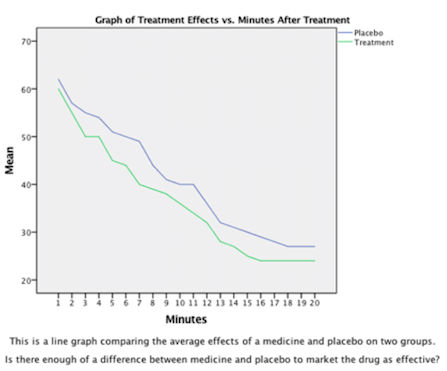
\includegraphics[width=6.5cm]{chapters/Chapter_9/ext_figure/timeVsRx.png} % requires the graphicx package
   % \caption{example caption}
   % \label{fig:example}
\end{figure}

When one of the comparison groups in a study is a control group or placebo, randomized trials are sometimes called randomized controlled trials, or randomized controlled experiments. As much as possible, researchers try to conduct double-blind randomized controlled trials, where neither doctor nor patient knows what treatment the patient is receiving. In the common cold example, some patients get a sugar pill or placebo while others get a new alternative medication thought to treat cold symptoms.  The important point to remember here is that in a double-blind controlled experiment both the patients and doctors have no idea if a patient is receiving the sugar pill/placebo or the cold medicine. This is achieved by giving each patient a pill that looks identical regardless as to whether it’s the inert placebo or the active medicine.

% \begin{minipage}[ht]{5cm}

\begin{figure}[ht]
   \centering

   
\includegraphics[width=3cm]{chapters/Chapter_9/ext_figure/placebo.png}
   
\includegraphics[width=3cm]{chapters/Chapter_9/ext_figure/medicine.png}
   % requires the graphicx package
    \caption{\textbf{Placebo} or \textbf{Medicine}.  Can you spot the difference? -- Single Blinding.
Can your doctor? -- Double Blinding. }
   % \label{fig:example}
\end{figure}
% \end{minipage}

This double-blinding is important because it offers additional protection against bias. In such studies, all groups have the same frame of mind (as opposed to knowing you are not really getting the new drug). Similarly, the experimenter has the same frame of mind evaluating patients from each group. You might wonder, isn't it enough to single-blind the study, to make sure that just the patients are unaware whether they received the placebo or medicinal pill? No, it is not. Imagine an experimenter who administers both the placebos and medications but does so knowing which is which. That researcher might unintentionally treat these two groups differently, perhaps just by spending an extra minute with patients from the medicated treatment group or by approaching them with a little more enthusiasm. It's this sort of unwitting behavior that can invite bias into the study.

\section{Observational studies}

In many cases, the treatments being compared cannot be assigned, and hence cannot be randomized.  The study involving women and leg fractures is an example.  We were comparing leg fracture rates of two comparison groups, men and women.  Whenever a new subject enters the study (by having a car accident), we observe what gender they belong to, instead of randomly assigning it.  Studies like these are called observational studies, as opposed to randomized experiments. In the hierarchy of scientific evidence, observational studies are not as strong as randomized trials, which is the gold standard. Since the subjects of observational studies assign themselves to their group, there may be selection bias that leads to confounders (like the women in the leg-fracture study being shorter).  Effects of known confounders can be controlled in analysis.  For example, we can compare leg fracture rates of men and women with the same heights. Investigators will need to anticipate potential confounders and control for them. We enumerate typical reasons for nonrandomized studies:

\begin{enumerate}
\item Assigning treatment is impossible (e.g., to compare fracture rates between men and women, we cannot randomize subjects into the comparison groups).

\item Assigning treatment is unethical (e.g. to compare cancer rates of smokers and nonsmokers, we do not want to randomize subjects into smoker-nonsmoker     comparison groups)

\item Assigning treatment is impractical (e.g. the outcome is a rare event like cancer or stroke, and a randomized trial would need too many subjects and too much time).  In cases like these, a case-control study is generally the way to go.
\end{enumerate}

\fbox{\parbox{14cm}{
\textbf{Observational} studies are conducted when randomization to treatment groups  \\ is impossible, unethical, or impractical.
}}

Returning to the leg-fracture example, we stick to observational studies in such a case for two reasons. As described above, it's impossible to perform the study any other way with the data collected. But we also should not elect to change the study, to collect the data in a different and randomized manner.  In other words, we should not even try to get the bias-reducing benefits of randomization because of ethical constraints. To perform randomized clinical trials in this study of leg fractures we would need to randomly select subjects whose legs would be broken for the sake of the study. Causing suffering like this is prohibited by several codes of ethics like the Nuremberg Code, a code of research ethics drafted after the Nuremberg trials of Nazi war criminals.  These criminals included scientists who designed and performed inhumane experiments. Beyond the official ban, though, such research is wrong in its causing excessive suffering and its infringement upon basic human rights.

Another reason we may conduct an observational study is that they can be more practical compared to randomized controlled trials. This can be due to the constraints of a rare disease, or the cost a randomized study would entail.  A researcher might want to study whether regular exercise can prevent a rare form of cancer.  Randomization and control here would require that we randomly select patients first, group them along exercise programs (say regular, irregular, and no exercise), and wait to see how the different groups respond (do the exercise groups have significantly fewer cases of cancer?).  This study might not work out at all because, since the cancer is rare, it's possible that no or very few of our subjects will get the cancer.  It also may take many years before cancer would appear.

This study would be quite time-consuming and labor-intensive. Imagine all the financial resources that would be required to do all that exercise-monitoring over all the patients and years! This brings us to our second point, that observational studies are practical because they tend to be less costly than randomized controlled trials. Companies often use statistics to generate revenue, but they tend to do this not by randomized experiments, but by analyses of marketing data they collect through sales or surveys. Nonrandom observational studies like analyses of sales data are an easy approach in that all they require are a data collection apparatus and a statistician. For instance, clothing designers want to keep up with trends in consumer spending, but might sell hundreds of different garments to thousands of outlets across the world. When sales of one item begin to slip, it might be difficult to notice amidst all the chaos of such a business enterprise. A statistician can help here by analyzing the proportions of revenue generated by each garment from month to month, and making recommendations about which products to push when. The statistician might even find style or color-based patterns that repeat themselves seasonally, allowing the company to adjust before their sales ever begin slipping.

\subsection{Case-control studies}

Instead of randomizing subjects into diet groups and then comparing the weight loss outcome, a case-control study would look for people in the population who lost weight, and then ask them what diet they used.  Thus, you start with the outcome, and then work back to the type of treatment.  These are also classified as retrospective studies, because they look back and compare weight loss or disease rates of various treatments.  Randomized experiments are necessarily prospective, in the sense that you randomize treatment and then later see which groups lost more weight or had more disease.

Case-control studies are frequently used because they are cheaper and easier to conduct, since it generally requires a survey of a database, instead of an expensive and time-consuming recruitment and handling of subjects.  There are plenty of successful case-control success stories in the scientific literature.
The first study formally linking lung cancer to smoking was a 1950 case-control study ``Smoking and Carcinoma of the Lung'' by Richard Doll and A. Bradford Hill
(British Medical Journal, 1950 September 30; 2(4682): page 739--748).  Using patients in 20 hospitals in London, they found that lung-cancer patients had higher rates of smokers than a comparable control group of patients.   For example, among district hospitals, 48 out of 98 lung cancer patients smoked 15 or more cigarettes daily.  In contrast, only 30 out of 98 non-cancer patients smoked 15 or more cigarettes daily.

In general, case-control studies are able to conclude a link or `association,' but are not able to prove `causation.'   However, case-control studies provide initial evidence that can generate resources for more rigorous studies like double-blind randomized controlled trials.  In the case of smoking and lung cancer, randomized trials are unethical, but given the eventual results of multiple studies, it is now accepted by the scientific community that smoking causes lung cancer.

\subsection{Case-crossover studies}

Sometimes, each subject can be their own control.  This is called a case-crossover study, because subjects in the treatment group ``crossover'' to the control group.
An example is a 1997 study linking cell phone use to car accidents: ``Association between cellular-telephone calls and motor vehicle collisions'' by D.A. Redelmeier and R.J. Tibshirani (The New England Journal of Medicine, 1997 Feb 13; vol 336, pp. 453-8).  The subjects were people who reported a collision to the North York Collision Reporting Centre between July 1, 1994, and August 31, 1995, Among these, 742 had cell phones and consented to participate in the study.  Instead of asking each person whether they were using their cell phone during the time of the collision (an unreliable method), the investigators examined their detailed phone billing records.  Their results are quoted below:

\begin{quotation}
Overall, 170 subjects (24 percent) had used a cellular telephone during the 10-minute period immediately before the collision, 37 (5 percent) had used the telephone during the same period on the day before the collision, and 13 (2 percent) had used the telephone during both periods. The crude analysis indicated that cellular-telephone activity was associated with a relative risk of a motor vehicle collision of 6.5 (95 percent confidence interval, 4.5 to 9.9).  The primary analysis, adjusted for intermittent driving, indicated that cellular-telephone activity was associated with a quadrupling of the risk of a motor vehicle collision (relative risk, 4.3; 95 percent confidence interval, 3.0 to 6.5).
\end{quotation}










\section{Key Words}

% \colorbox{lgray}{\parbox{15cm}{
% \begin{minipage}[ht]{6cm}
% \begin{itemize}
% \item Independent random samples
% \item Pooled estimate
% %\item $\sigma_{p-p^*}$
% %\item $\sigma_{\bar{x} - \bar{x}^*}$
% \end{itemize}
% \end{minipage} \hfill
% \begin{minipage}[ht]{6cm}
% \begin{itemize}
% %\item Independent random samples
% %\item Pooled estimate
% \item $\sigma_{p-p^*}$
% \item $\sigma_{\bar{x} - \bar{x}^*}$
% \end{itemize}
% \end{minipage}
% }}

% \newpage
\twocolumn
\section{Exercises}

\begin{exercises}

  \begin{exercise} %1

Give some examples of \\ studies where:

\begin{enumerate}
\item a randomized trial is impossible
\item a randomized trial is impractical \\ because of length of time the study      \\ would require
\item a randomized trial is impractical \\ because of the number of subjects \\ the study would require
\end{enumerate}


	\end{exercise}
	\begin{solution}  % 1

	  $H_0: \mu_1 = \mu_2$ vs. $H_0: \mu_1 \neq \mu_2$
	\end{solution}

  \begin{exercise} % 2

Suppose a doctor is interested in investigating the causes of an \\ extremely rare disorder that occurs in only 0.00001\% of men.  What type of study would be necessary to firmly establish the causes of the disease?  Is this type of study an appropriate choice for such a disease?  Why or why not?

	\end{exercise}
% 	\begin{solution}  % 2
% <<label=lbl9-2, results='asis', echo=FALSE>>=
%   cv1 <- sprintf('%.4f', (qt(p=0.95, df=10)))
% @
%
% 	  From the t-distribution table, choose df row 10 and column significance level 0.05. \\
% 	  Student's $t$ distribution, $CV = cv1$
% 	\end{solution}

  \begin{exercise} % 3

What is a double-blind \\ study?  Give an example where double- \\ blinding is not possible.

    \end{exercise}
    \begin{solution}  % 3

The test statistics is $|-1.66|$ and significance level is 1.8125.  Since the test statistic is less than the significance level, fail to reject $H_0$.
    \end{solution}

  \begin{exercise} % 4

Some recent research has \\ shown that patients who know they have \\ taken nothing more than an inert sugar pill still experience the placebo effect. Briefly describe a study design that might replicate \\ these results. What type of study would you choose? What different groups would be \\ needed?



  \end{exercise}
  % \begin{solution}  % 4
  %
  %   $H_0: P_1 = P_2$ vs. $H_A: P_1 \neq P_2$
  % \end{solution}

  \begin{exercise} % 5

What is the advantage of case-control studies over clinical trials?

  \end{exercise}
  \begin{solution}  % 5


    Standard Normal (z) distribution, $Z = \pm 1.96$.
  \end{solution}

  \begin{exercise} % 6

A football organization is \\ concerned about the number of injuries to its athletes during games. The organization designs an observational study to help decide on rule changes that will reduce the risk of injury to players. They collect data and observe that a very high proportion of injuries are incurred during the first moments of the game during kickoff. The organization thus entertains the idea of changing the rules governing kickoffs. Are there any hidden confounders that the organization should address before making changes to kickoff rules? What are they, and how might they be addressed?

	\end{exercise}
	% \begin{solution}  % 6
	%
	%   Conclude that there is a difference, since the test statistic (z = 2.04) is greater than the critical value (z = 1.96).  Therefore, reject $H_0$
	% \end{solution}

	  \begin{exercise} % 7

What is the advantage of clinical trials over case-control studies?

  \end{exercise}
  \begin{solution}  % 7

    $H_0: P_1 = P_2$ vs. $H_A: P_1 > P_2$
  \end{solution}

\end{exercises}
\onecolumn


%!Rnw root = ../../Master.Rnw

\chapter{The Normal Distribution}
\label{chap:ch6}

\section{Objective}

After completing this part, students should be able to:

\fbox{\parbox{14cm}{

\begin{itemize}
\item Define and explain the concept of the {\textbf{Normal Curve}}.
\item Convert empirical scores to z-scores and use z-scores and the Normal Distribution curve table to find areas above, below and between points of the curve and  express them regarding their probabilities.
\item Utilize the standard normal distribution to solve probability (chance) problems.
\end{itemize}
}}

\section{Using the normal curve} \index{Normal Curve}

Best Buy wants to know how many smart fitness and GPS watches (like Fitbit, Garmin, and Apple) to order for their Kalamazoo location. Past data show that this time of year, they sell an average of 36 fitness watches per month, with a standard deviation of 8.

\subsubsection{Problem 1.}  If they order 40 watches, what is the probability that they will run out of stock?

\subsubsection{Problem 2.}  Given the cost of running out of stock and the storage cost of keeping too many, the manager decides to order enough smart watches to cover customer demands 90\% of the time, i.e there should be 10\% or less likelihood that they run out of stock. How many should they order?

Knowing the average and SD of a process $(36 \pm 8)$ gives us some understanding of what to expect.  However, the sales situation above requires the computation of probabilities, or chances, as in the ``chance of demand exceeding 40.''   This desired probability is the shaded area to the right of 40 under the histogram of demand (see the first graph in Figure 4.1).  Does this look like 0.20 of the total area?  0.30?  0.40?

\begin{figure}[ht]
\caption{Probability of Demand exceeding 40}


{\centering 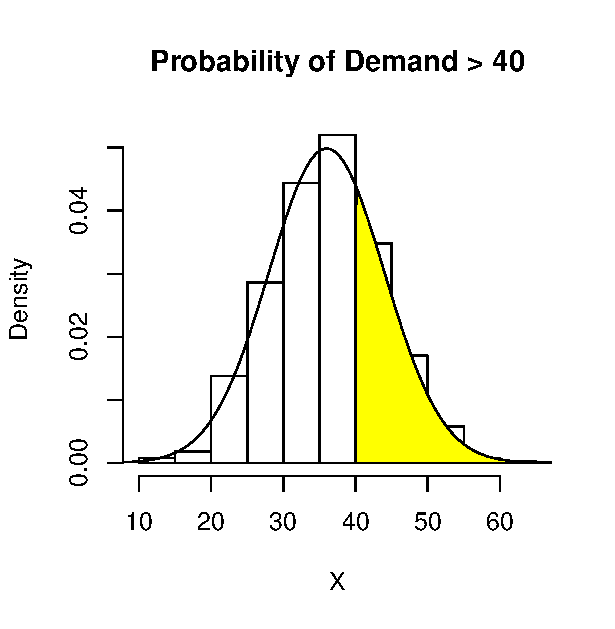
\includegraphics[width=8cm]{figure/LBL4a-1} 

}



\end{figure}

The normal curve (or bell curve) is useful in helping us calculate probabilities like these.  If we smooth out the top of the histogram in Figure 4.1, it will look like a normal curve.  More precisely, it will look like a normal curve with a mean of 36 and an SD of 8, denoted as $N(36, 8)$.  So the shaded area on the left will be approximated by the shaded area under the $N(36, 8)$ curve on the right.  Do the two shaded areas look about the same?

Of course, the areas look similar because in our example, the histogram on the left
looks like a normal curve.  It does not have to.  If it does not, then the approximation of areas using the normal curve will be bad.  The normal curve approximation should be used with caution.

\subsubsection{The Standard Normal or Z Curve}

The standard normal curve (or Z-curve) looks like Figure 4.2, and has the following properties:

\begin{center}
\fbox{\parbox{10cm}{
  \begin{enumerate}
  \item center is at zero
  \item The area under the curve satisfies the following: \\
  The area between -1 and +1 is 0.68 \\
  The area between -2 and +2 is 0.95 \\
  The area between -3 and +3 is 0.997 \\
  The area between $- \infty$ and $+ \infty$is 1.00
  \end{enumerate}
}}
\end{center}

\begin{figure}[ht]
\caption{Normal Z-curve}



{\centering 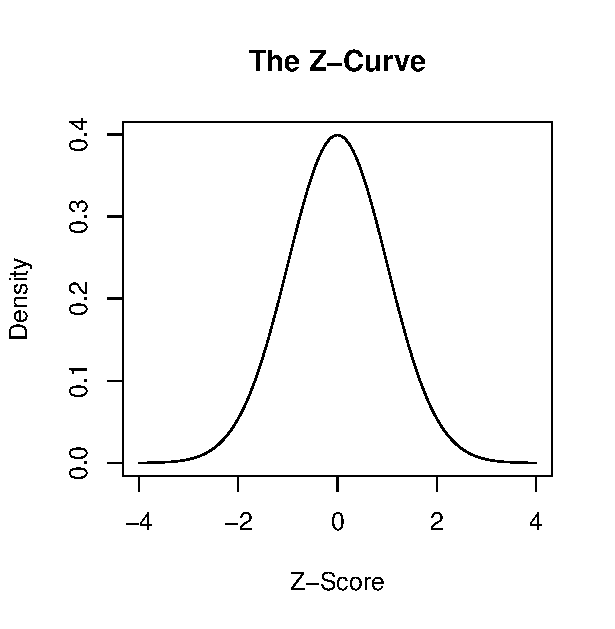
\includegraphics[width=8cm]{figure/LBL4b-1} 

}



\end{figure}

In general, any area under the curve can be found using the Z-table on page 46 at the end of this chapter.

\begin{minipage}[ht]{3cm}

\textbf{For practice}
\end{minipage}
\begin{minipage}[ht]{6cm}

\parbox{6cm}{
  Using the Z-table, find $\dots$

  \begin{enumerate}
  \item the area to the left of 1.2
  \item the area to the left of 1.25
  \item the area to the right of 1.25
  \item the area to the left of -1.25
  \item the area between 1.25 and 2.50
  \end{enumerate}
}
\end{minipage}

Are we ready to find the area under the normal curve in Figure 4.1?  Not yet.  The horizontal axis in Figure 4.1 is wrong for the Z-table, it does not have a mean of 0 and an SD of 1. Instead, it has a mean of 36 and an SD of 8.  The trick is to replace the $N(36, 8)$ horizontal axis with a $N(0, 1)$ axis, labeled Z.  See Figure 4.3.  Note that $Z = 1$ whenever X is one SD above the mean.  Similarly, $Z = -1$ whenever $X$ is one SD below the mean.  In general, Z is related to $X$ as follows:

  \begin{equation} Z = \frac{X - mean}{SD} \end{equation}

\begin{figure}[ht]

\caption{Areas within one and two SD's of the Mean \textit{N(36, 8)}}

\begin{minipage}[ht]{7cm}



{\centering 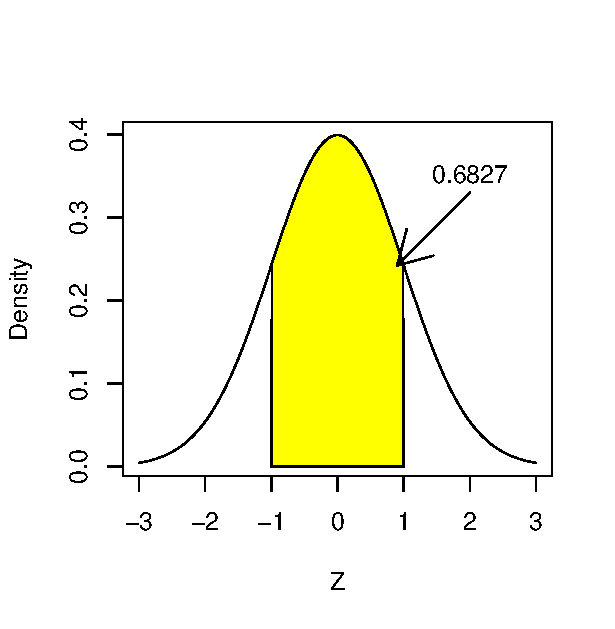
\includegraphics[width=4cm]{figure/LBL4c1-1} 

}



\end{minipage}
\begin{minipage}[ht]{7cm}


{\centering 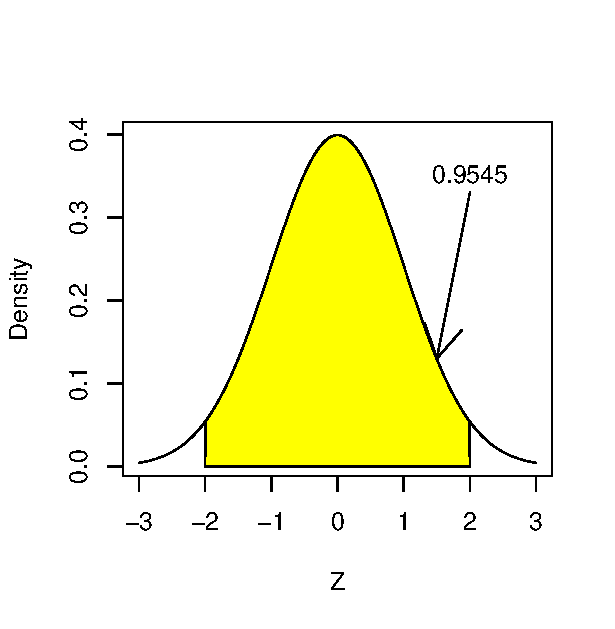
\includegraphics[width=4cm]{figure/LBL4c2-1} 

}



\end{minipage}
\end{figure}

What is the probability of demand exceeding 40?  This is the area under the curve to the right of $X = 40$ or $Z = 0.5$ (see Figure 4.4).  Using the $Z$-table, this area is $1 -  0.6915 = 0.3085$.

\begin{figure}[ht]

\caption{$P[ X \ge 40 ]$ }

\begin{minipage}[ht]{7cm}



{\centering 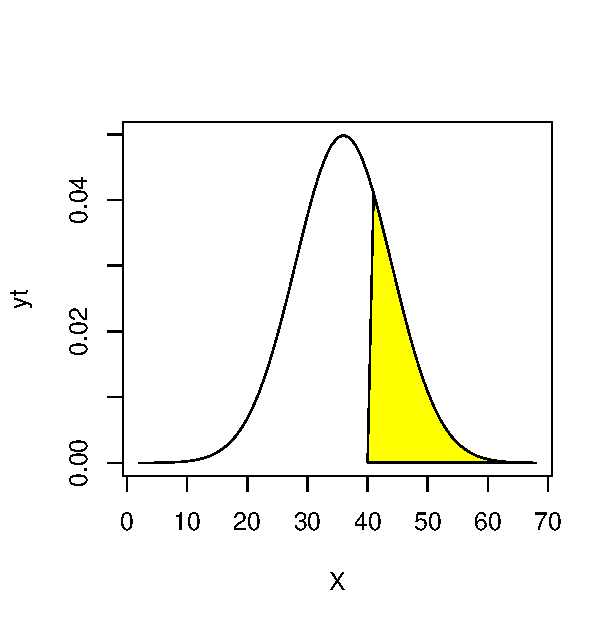
\includegraphics[width=4cm]{figure/LBL4d1-1} 

}



\end{minipage}
\begin{minipage}[ht]{7cm}


{\centering 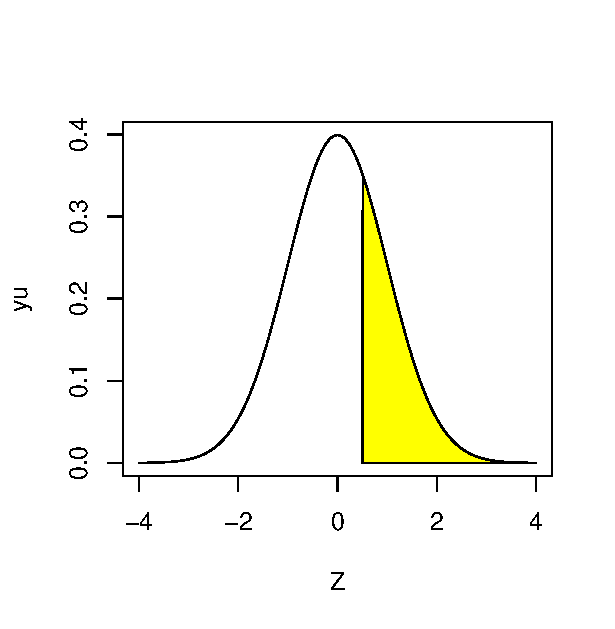
\includegraphics[width=4cm]{figure/LBL4d2-1} 

}




\end{minipage}
\end{figure}

\section{Calculating percentiles}

We restate Problem 2 given at the start of the chapter.

\textbf{Problem 2.} Given the cost of running out of stock and the cost of having too many, the manager decides to order enough smart watches to cover customer demands 90\% of the time, i.e there should be 10\% or less likelihood that they run out of stock.  How many should they order?

We want to estimate the number of smart watches so that there is only a 10\% chance of running out.  Note that this is the 90th percentile of demand.

Looking at Figure 4.5, we see that we need to shade the upper 10\% of the area under the histogram.  What X value corresponds to the boundary?  Using the normal table, the Z value 90th percentile is 1.28.  What X value corresponds to Z = 1.28?  We solve equation 4.1 backwards.

\begin{eqnarray*}
1.28 & = & \frac{X - 36}{8}  \\
36 + 1.28(8) & = & X-36 + 36 \\
36 + 1.28(8) & = & X \\
X & = & 46.24
\end{eqnarray*}

The manager should have at least 46 smart watches in the store.

\begin{figure}[ht]
\caption{The 90th Percentile: $P[X \ge a] = 0.10$ }


{\centering 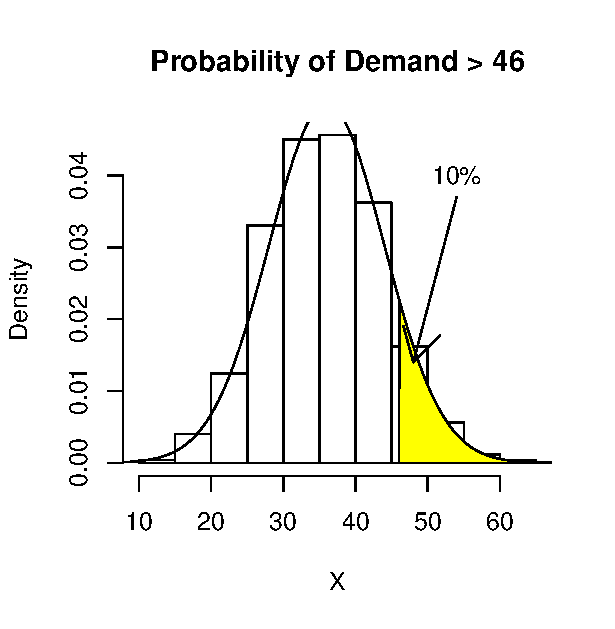
\includegraphics[width=8cm]{figure/LBL4e-1} 

}



\end{figure}

\section{Calculating symmetric tail areas}

In later sections, we will need to calculate tail areas (or $P$-values).  For example, how frequently does a normal variable fall outside of 2.25 SD from the center?  We know a random variable following a normal distribution falls within 1 SD from the center 68\% of the time, and hence outside of 1 SD from the center only 32\% of the time.  What about 2.25 SD?

The area outside of 2.25 SD from the center is the combined area left of -2.25 and right of 2.25.  From the $Z$-table, the area to the right of 2.25 is 1 - 0.9878 = 0.0122.  Therefore, the combined tail areas is 0.0122 + 0.0122 = 0.0244.  A random variable following a normal distribution falls outside of 2.25 SD from the center only 2\% of the time.

\begin{minipage}[ht]{3cm}

\textbf{For practice}
\end{minipage}
\begin{minipage}[ht]{6cm}

\parbox{6cm}{
  What percentage of time does \\ a normal variable fall outside:

  \begin{enumerate}
  \item 0.4 of the mean
  \item 1.4 SD of the mean
  \item 2.4 SD of the mean
  \item 3.4 SD of the mean
  \end{enumerate}
}
\end{minipage}

\section{The Empirical Rule}

Figure 4.3 provides a useful interpretation of the SD.  It is stated as follows:

\fbox{\parbox{12cm}{
\textbf{Empirical Rule:} \\
If the data histogram is approximately bell-shaped, expect around \\
68\% of the observations will fall within \textbf{one} SD of the mean  \\
95\% of the observations will fall within \textbf{two} SD of the mean  \\
99.7\% of the observations will fall within \textbf{three} SD of the mean
}}


\twocolumn

\section{Exercises}

\begin{exercises}

  \begin{exercise} % 1

A study was conducted in order to determine if any link existed between cellular phone usage and the development of brain cancer (don't worry, no connection was found).  Data from this study indicate that the daily cell phone usage for all users is approximately normally distributed with mean 2.4 hours and standard deviation 1.1 hours.

	\begin{enumerate}
	\item What proportion of cell phone users are on their phones between 1 hour
and 3 hours per day?
  \item Just to be safe, suppose you decide to be in the 5th percentile of
cell phone users in terms of monthly usage.  How much time can you spend on your phone per day?
	\end{enumerate}

   % \framebox[5cm][l]{ Answer: }
	\end{exercise}
	\begin{solution}  % 1


\begin{enumerate}
	\item The proportion of cell phone users are on their phones between 1 hour
and 3 hours per day is 0.6057221
  \item Just to be safe, suppose you decide to be in the 5th percentile of
cell phone users in terms of monthly usage.  How much time can you spend on your phone per day? You decide to spend no more than 35.4396606 minutes on your phone per day.
	\end{enumerate}
	\end{solution}

  \begin{exercise} % 2

On the average, a watch battery is known to last for 2 years (24-months), with a standard deviation of 9 months.  \\ Assuming that the population is normally distributed,

 \begin{enumerate}
	\item What percentage of watch  batteries  last \\ more than 6 months?
	\item What is the life span of a watch battery which lasts longer than 60\% of all batteries?
	\item What proportion of watch batteries last \\ shorter than 2 years or longer
than 3 1/2 years (42 months)?
 \end{enumerate}

	\end{exercise}
	\begin{solution}  % 2



\begin{enumerate}
	\item The percentage of watch batteries last more than 6 months is $P[ X > 6] = 0.998067$.
	\item What is the life span of a watch battery which lasts longer than 60\% of all batteries?  $P[X > a] = .60$. Now solve for a = 21.7198761.
	\item What proportion of watch batteries last shorter than 2 years or longer
than 3 1/2 years (42 months)?
$P[X < 24] + P[X > 42] = .5 + 0.0227501 = 0.5227501$
 \end{enumerate}

	\end{solution}

  \begin{exercise} % 3

Suppose 95\% of data coming from a normally distributed population falls between 4 and 35.  Based on the empirical rule, what is the standard deviation of this sample of data?

  \end{exercise}
  \begin{solution}   % 3



    The standard deviation is $SD = \frac{35 - 4}{4} = 7.75$
  \end{solution}

	\begin{exercise}  % 4

A random variable is normally distributed with mean of 10 and standard deviation of 2.

\begin{enumerate}
\item What is the probability the value is \\ greater than 6?
\item What is the probability the value is less than 12?
\item What is the probability the value is between 6 and 12?
\item 33\% is above what value?
\item 33\% is below what value?
\end{enumerate}

	\end{exercise}
	\begin{solution}  % 4


\begin{enumerate}
\item The probability the value is greater than 6 is $P[X > 6] = 1$
\item The probability the value is less than 12 is $P[X < 12] = \ensuremath{3.3976731\times 10^{-6}}$
\item The probability the value is between 6 and 12 is $P[ 6 < X < 12] = 0.9999966$
\item 33\% is above a, i.e., $P[X > a] = .33; a = 10.8798263$
\item 33\% is below b, i.e., $P[X < b] = .33; b = 9.1201737$
\end{enumerate}
	\end{solution}

  \begin{exercise}	% 5

The stock price for \\ Coca-Cola (KO) is normally distributed with a mean of 42.14 and standard deviation of 1.43.

\begin{enumerate}
\item What is the probability that the stock price is between 39.88 and 46.01?
\item What is the probability that the stock price is above 40?
\item What is the probability that the stock price is below 40?
\end{enumerate}

  \end{exercise}
\begin{solution}  % 5


\begin{enumerate}
\item The probability that the stock price is between 39.88 and 46.01 is $P[39.88 < X < 46.01] = 0.9395927$.
\item The probability that the stock price is above 40 is $P[X > 40] = 0.9327388$.
\item The probability that the stock price is below 40 si $P[ x < 40] = 0.0672612$.
\end{enumerate}
\end{solution}

\begin{exercise}  % 6

The average adult female \\ height is 63.8 inches with a standard deviation of 2.40. Assume the distribution is approximately normal.

\begin{enumerate}
\item What proportion of adult female heights is below 72?
\item 25\% of adult females are greater than what height?
\end{enumerate}

  \end{exercise}
\begin{solution}  % 6


\begin{enumerate}
\item The proportion of adult female heights is below 72 is $P[ X < 72] = 0.999683$.
\item 25\% of adult females are greater than $P[ X > a] = .25$ where a = 65.4187754
\end{enumerate}
\end{solution}

\begin{exercise} % 7

Values in the table give the area under the curve to the left of the z-values on the margins.  The upper margin gives the hundredth digit of z.  For example:

\begin{enumerate}
\item The area to the left of 0.0 is ?
\item The area to the left of 0.2 is ?
\item The area to the left of 0.25 is ?
\item The area to the left of 2.25 is ?
\end{enumerate}

	\end{exercise}
\begin{solution}  % 7

\begin{enumerate}
\item The area to the left of 0.0 is.5000
\item The area to the left of 0.2 is.5793
\item The area to the left of 0.25 is.5987
\item The area to the left of 2.25 is.9878
\end{enumerate}
\end{solution}

\end{exercises}

 \onecolumn



%!Rnw root = ../../Master.Rnw

\chapter{The Binomial Distribution}
\label{chap:ch7}

\section{Objective}

After completing this part, students should be able to:

\fbox{\parbox{14cm}{
\begin{itemize}
\item Explain the purpose of inferential statistics.

\item Define and explain the basic techniques of random sampling.

\item Explain and define these key terms:
	\begin{itemize}
	\item Population
	\item Parameter
	\item Sample
	\item Statistic
	\item Equal Probability of SElection Method.
	\end{itemize}

\item Differentiate between the sampling distribution, the sample, the  population.

\item Explain the two theorems presented.

\end{itemize}
}}

\section{Binomial Probabilities}

A sequence of n observations is called a binomial process if

\begin{enumerate}
\item each observation results in one of two possible outcomes (which we call    success and failure)
\item the probability of success is p and the probability of failure is q = 1 - p for all observations
\item the observations are independent of each other.
\end{enumerate}

\begin{center}
\begin{tabular}{@{} ccccc @{}} \hline
Obs 1 & Obs 2 & Obs 3 & $\cdots$ & Obs n \\
$p \swarrow  \searrow q$ & $p \swarrow  \searrow q$ & $p \swarrow  \searrow q$ & & $p \swarrow  \searrow q$ \\
S \hspace{3mm}   F & S  \hspace{3mm}  F &  S  \hspace{3mm}  F &  & S \hspace{3mm}   F \\ \hline
\end{tabular}
\end{center}

Let X denote the total number of successes among the n observations.  Then
X is called a \textbf{binomial random variable} \index{binomial random variable} with parameters n and p. The following are all binomial random variables.

\subsubsection{Example 1} A Stat 1600 multiple choice quiz has 5 questions, with each question having 5 choices.  Let X be the number of correct answers (C) by someone who is guessing on all questions.  Then X is a binomial random variable with parameter values n = 5 and p = 0.2.

\begin{center}
\begin{tabular}{@{} ccccc @{}} \hline
Ques 1 & Ques 2 & Ques 3 & Ques 4 & Ques 5 \\
$.2 \swarrow  \searrow .8$ & $.2 \swarrow  \searrow .8$ & $.2 \swarrow  \searrow .8$ & $.2 \swarrow  \searrow .8$ & $.2 \swarrow  \searrow .8$ \\
C \hspace{3mm} W & C  \hspace{3mm}  W &  C  \hspace{3mm}  W &   C \hspace{3mm} W & C \hspace{3mm}   W \\ \hline
\end{tabular}
\end{center}

\subsubsection{Example 2} Available data shows that 40\% of telephone respondents agree to be interviewed for market research surveys.  Suppose that the polling organization Reliable Research randomly selects and dials telephone numbers until 50 respondents are reached.  Let X be the number of respondents (out of the 50) who agree to be interviewed.  Then X is a binomial random variable with parameter values n = 50 and p = 0.40.

\subsubsection{Example 3} Historically, 20\% of buyers at Best Buy who purchase smart fitness and GPS watches (like Fitbit, Garmin, and Apple) also purchase the Geek Squad’s protection plan.  Suppose that 300 smart fitness watches were sold during the previous quarter.  Let X be the number of extended protection plans that were sold along with the 300 smart watches.  Then X is a Binomial random variable with parameter values n = 300 and p = 0.20.

\section{Computing Binomial Probabilities}

In Example 1, the number of correct guesses may be 0, 1, 2, 3, 4, or 5.  How likely can a guesser get all 5 questions right? The answer is 0.0003, or about three times in 10000 attempts.  How about the likelihood of getting 2 out of 5 questions right?  The answer is .2048, about a fifth of the time.  The following \textbf{probability distribution table} gives the likelihood or probability of each possible value of X.



\begin{center}
\begin{tabular}{@{} cccccc @{}} \hline
$P[X = 0]$ & $P[X = 1]$ & $P[X = 2]$ & $P[X = 3]$ & $P[X = 4]$ & $P[X = 5]$ \\ \hline
0.32768 & 0.4096 & 0.2048 & 0.0512 & 0.0064 & \ensuremath{3.2\times 10^{-4}} \\ \hline
\end{tabular}
\end{center}

You can compute these probabilities yourself by successively substituting \\ $j = 0, 1, 2, 3, 4, \texttt{ and } 5$ in the formula

\begin{equation*}
 P[ X = j] = \frac{5!}{j! (5 - j)!} .2^j .8^{5 - j}, \texttt{ where j = 0,1,2,3,4,5 }
 \end{equation*}

Remember that 0! = 1 and (0.2)0 = 1.  This formula is called the \textbf{binomial probability distribution function (pdf)} for $n = 5$ and p$ = 0.2$.  To compute the probabilities for Examples 2 and 3, you will need the binomial pdf for general $n$ and $p$:

\begin{equation*}
 P[ X = j] = \frac{n!}{j! (n - j)!} p^j q^{n - j}, \texttt{ where j = 0,1,2, $\cdots$ , n}
 \end{equation*}


\subsubsection{Example 3} (Cont.):  10 smart fitness and GPS watches were sold in one day.  What is the probability that 3 extended Geek Squad protection plans were sold?  Using the equation above with $n = 10, p = 0.20$, and $j = 3$, we get

\begin{equation*}
 P[ X = 3] = \frac{10!}{3! (10 - 3)!} .2^j .8^{10 - 3} = 0.201
 \end{equation*}

\begin{minipage}[ht]{3cm}

\textbf{For practice}
\end{minipage}
\begin{minipage}[ht]{12cm}

Five percent of video games rented at Gamers Retro Rental are returned late. If 30 video games were rented during the last hour, what is the probability that

\begin{enumerate}
\item 2 will be returned late
\item none will be returned late
\item 2 or fewer will be returned late
\item 5 or more will be returned late
\end{enumerate}
\end{minipage}

\section{Expected Value and SD of a Binomial Random Variable}

Suppose that last quarter, Best Buy sold 300 Smart fitness watches.  If there is 0.20 likelihood of selling an extended protection plan with each smart watch, the number of extended protection plans sold last quarter should be around 60 give or take 7 or so (we will compute this later).

The first number is called the expected value of the number of protection plans sold; the second number is the standard deviation.  Recall that X, the number of protection plans sold, is a \textbf{Binomial random variable}.  The \textbf{expected value}, denoted \textbf{E(X)}, of a binomial random variable X with parameters n and p is computed as:

\begin{equation*}
E[ X ] = np
\end{equation*}

The expected value $E(X)$ is also called the average or mean of X, and denoted $\mu$.  The standard deviation, denoted $SD(X)$ or $\sigma_x$, of a binomial random variable is computed as:

\begin{equation*}
SD(X) = \sigma_x = \sqrt{npq}
\end{equation*}

Returning to the example, since $n = 300$ and $p = 0.20$, we have $E(X) = 300(0.20) = 60$, and $SD(X) = \sqrt{300(0.20)(0.80)} = 6.93$, or approximately $60 \pm 7$.

The SD for random variables is interpreted similarly to the SD for a sample.  If the store sells 300 smart watches sets every quarter, they won't sell exactly 60 Geek Squad protection plans every time; sometimes they will sell more, sometimes they will sell less.   By how much more, and how much less?  The answer is, ``By 7, on average.''   Similarly, a baseball player with 0.200 batting average won't necessarily get 60 hits in 300 at bats.  We expect him to get 60 hits, give or take 7 hits.

\begin{minipage}[ht]{3cm}

\textbf{For practice}
\end{minipage}
\begin{minipage}[ht]{12cm}

Suppose that 5\% of video games rented at Gamers Retro Rental incur a late rental fee. If 700 videos were rented last week, the number that will incur a late rental fee should be around \underline{\phantom{xxxxxxxxxx}} give or take \underline{\phantom{xxxxxxxxxx}}.

\end{minipage}

\section{Computing Binomial Probabilities Using the Normal Curve}

Beyond the empirical rule, we may apply the normal curve to approximating binomial probabilities.  The key image is a plot of binomial probabilities as a histogram.  For example, Figure 5.1 is a histogram of binomial probabilities for $n = 30$ and $p = 0.4$.

The height of the rectangle over, say 10, is its probability $P[X = 10$.  However, since the width of the rectangle is 1, then

\begin{equation*}
P[X = 10] = \texttt{ height of rectangle over 10 = area of rectangle over 10}
\end{equation*}

What about $P[X \le 10]$?  This probability corresponds to the total area of the rectangles over and to the left of 10 (shaded rectangles in Figure 5.2)

Using the binomial probability function to compute the area (probability) of each
shaded rectangle, the total area equals 0.2915.  However, this requires repeated applications of the binomial formula (11 times, in fact).  We may calculate a quick approximation of the desired probability by replacing the rectangles with a curve!  See shaded area under curve in Figure 5.2.

There are infinitely many normal curves, which one do we use to replace the rectangles?  Answer: the one with the same mean and SD as the rectangles!  The (binomial) rectangles have a \textbf{mean}:

\begin{equation*}
\mu = np = (30)(.4) = 12
\end{equation*}

The (binomial) rectangles have a SD:

\begin{equation*}
\sigma = \sqrt{npq} = \sqrt{(30)(.4)(.6)} = 2.68
\end{equation*}

Using the normal curve with the same mean and SD, the area to the left of 10.5 is 0.2877, which is a close estimate of the true area of 0.2915.

Similarly, $P[X = 14] = 0.1101$ is approximated by 0.1115, the area under the normal curve between 13.5 and 14.5.

\begin{figure}[ht]
\caption{Histogram of Probabilities for Binomial n = 30 and p = 0.4}


{\centering 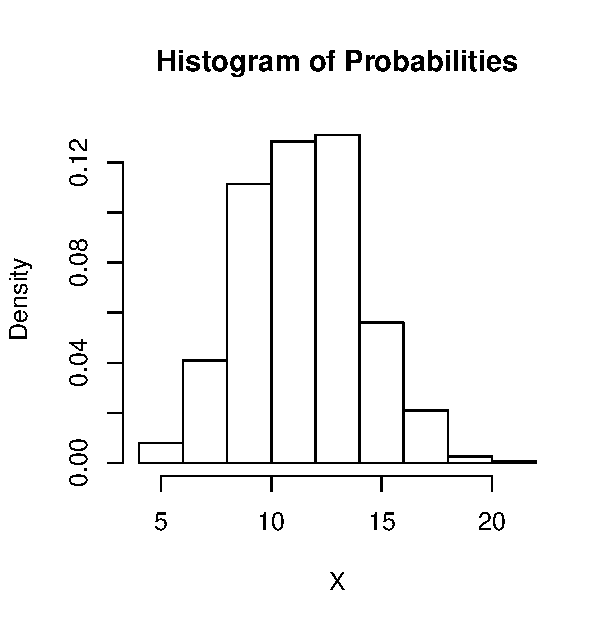
\includegraphics[width=11cm]{figure/LBL5b-1} 

}



\end{figure}


\begin{figure}[ht]
\caption{Approximating $P[X \le 10]$ using Curve instead of Rectangles}



{\centering 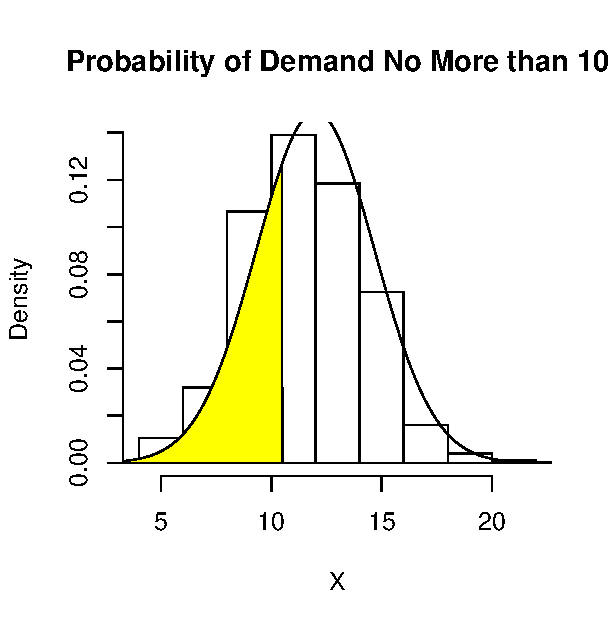
\includegraphics[width=11cm]{figure/LBL5c-1} 

}




\end{figure}

\section{Some Approximations Are Better Than Others}

Examine the shape of the binomial histogram for n = 20 and p = 0.10 in Figure 5.3.

\begin{figure}[ht]
\caption{Histogram of Probabilities for Binomial n = 20 and p = 0.10}


{\centering 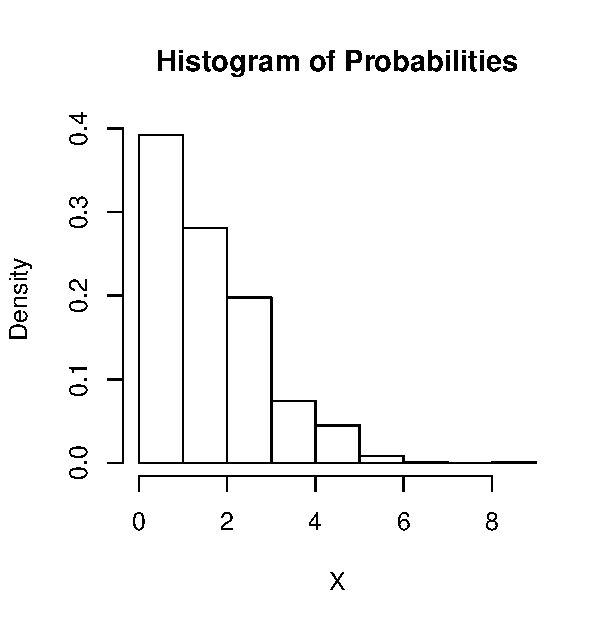
\includegraphics[width=11cm]{figure/LBL5d-1} 

}



\end{figure}

Since the curve is right skewed, we will get a poor approximation of areas if we replace the rectangles by a normal curve.  If the value of p were 0.90 instead of 0.10, the binomial histogram would be left skewed.  This is typical behavior of binomial histograms whenever $p$ is either too close to 0 or too close to 1.  When is it `safe' to use the normal curve to approximate binomial probabilities?  A convenient rule of thumb is as follows:

\fbox{\parbox{14cm}{
The \textbf{Normal Curve gives reasonable approximations} of binomial probabilites whenever both $np > 5$ and $nq >5$.
}}

The reader is reminded that normal curve approximations, no matter how close, are still approximations.  The binomial formula should be used to calculate exact probabilities whenever possible.

\twocolumn

\section{Exercises}

\begin{exercises}

  \begin{exercise} % 1

A binomial random variable \\ with a probability of success of 0.5 and 10 \\ observations. Assume each observation is \\ independent.

	  \begin{enumerate}
	  \item What is the mean and standard deviation?
    \item What is the probability that there are \\ more than 5 successes?
    \item What is the probability that there are \\ fewer than 5 successes?
    \item What is the probability that there are \\ between 1 and 3, inclusive?
	  \end{enumerate}

   % \framebox[5cm][l]{ Answer: }
	\end{exercise}
	\begin{solution}  % 1


		\begin{enumerate}
	  \item The mean and standard deviation are 5 and 1.5811388, respectively.
    \item The probability that there are more than 5 successes is $P[ X > 5 ] = 0.3769531$.
    \item The probability that there are fewer than 5 successes is $P[ X < 5 ] = 0.3769531$.
    \item The probability that there  are between 1 and 3 successes  is $P[ 1 \le X \le 5 ] = 0.1708984$.
	  \end{enumerate}
	\end{solution}

  \begin{exercise} % 2

A statistics exam contains 10 questions with 5 multiple choice options per question. By guessing on all questions,

\begin{enumerate}
\item What is the probability that at least 2 questions correct?
\item What is the probability that at most 2 questions correct?
\item What is the probability that between 1 and 3?
\end{enumerate}
	\end{exercise}
	\begin{solution}  % 2


\begin{enumerate}
\item The probability that at least 2 questions are correct is $P[X \ge 2] = 0.6241904$.
\item The probability that at most 2 questions arecorrect is $P[X \le 2] = 0.6777995$.
\item The probability that there  will be between 1 and 3 questions is $P[1 \le X \le 3] = 0.7717519$.
\end{enumerate}
	\end{solution}

  \begin{exercise} % 3

Apple's smart phone market \\ share is  0.146. If Apple conducts a nationwide survey of 651 smart phone users,

\begin{enumerate}
\item What is the probability that at least 100 of the people are Apple users?
\item What is the probability that at most 100 of the people are Apple users?
\item What is the probability that between 80 and 120?
\end{enumerate}
	\end{exercise}
	\begin{solution}  % 3


\begin{enumerate}
\item The probability that at least 100 people are Apple users is $P[X \ge 100] = 0.3070581$.
\item The probability that at most 100 people are Apple users is $P[X \le 100] = 0.7302684$.
\item The probability that between 80 and \\ 120 people are Apple users is $P[ 80 \le X \le 120] = 0.9572505$.
\end{enumerate}
	\end{solution}

  \begin{exercise} % 4

When rolling a die 10 \\ times,

\begin{enumerate}
\item What is the probability of rolling a 6 no more than 3 times?
\item What is the probability that no less than 3 times?
\end{enumerate}
	\end{exercise}
	\begin{solution}  % 4



\begin{enumerate}
\item The probability of rolling a 6 no more than 3 times is $P[X \le 3] = 0.9302722$.
\item The probability that no less than 3 times is $P[X \ge 3] = 0.2247732$.
\end{enumerate}
  \end{solution}

  \begin{exercise} % 5

The career batting average of Ty Cobb is 0.3664. If Ty Cobb had 8 at bats during a doubleheader,

\begin{enumerate}
\item What is the probability that he gets at least 7 hits?
\item What is the probability that at most 1 hits?
\item What is the probability that between 4 and 6?
\end{enumerate}
	\end{exercise}
	\begin{solution}  % 5


\begin{enumerate}
\item The probability that he gets at least 7 hits is $P[X \ge 7] = 0.0048184$.
\item The probability that he gets at most 1 hit is $P[X \le 1] = 0.1461307$.
\item The probability that he gets between 4 and 6 hits is $P[4 \le X \le 6] = 0.3245785$.
\end{enumerate}

  \end{solution}

	\begin{exercise}  % 6

Fill in the blanks. The probability of picking the Powerball number is \\ 0.0254. If 50 tickets are purchased, around \underline{\phantom{xxxxxxxx}} of  tickets will be winners,  give or take  \underline{\phantom{xxxxxxxx}}.    Assume each pick is independent.
	\end{exercise}
	\begin{solution}  % 6


The expected value is 1.27 and SD is 1.1125385

	\end{solution}

		\begin{exercise}  % 7

Fill in the blanks. The probability of a defective light bulb is 0.04. If purchase order of 200 bulbs is submitted, the number of defective light bulbs in the shipment is around \underline{\phantom{xxxxxxxx}}, give or take \\ \underline{\phantom{xxxxxxxx}}. Assume each light bulb is independent.
	  \end{exercise}
	  \begin{solution}  % 7


The expected value is 8 and SD is 2.7712813
	\end{solution}

%
\end{exercises}
\onecolumn



%!Rnw root = ../../Master.Rnw

\chapter{Sampling Distribution of the Proportion}
\label{chap:ch8}

\section{Objective}

After completing this part, students should be able to:

\fbox{\parbox{14cm}{
\begin{itemize}
\item Explain the purpose of inferential statistics.
\item Define and explain the basic techniques of random sampling.
\item Explain and define these key terms:
	\begin{itemize}
	\item Population
	\item Parameter
	\item Sample
	\item Statistic
	\item Equal Probability of SElection Method.
	\end{itemize}

\item Differentiate between the sampling distribution, the sample, the  population.
\item Explain the two theorems presented.
\end{itemize}
}}

\section{The Sample Proportion}

Suppose a student guesses at the answer on every question in a 300-question exam.  If he gets 60 questions correct, then his proportion of correct guesses is $60/300 = 0.20$.  If he gets 75 questions correct, then his proportion of correct guesses in $75/300 = 0.25$.  The proportion of correct guesses is simply the number of correct guesses divided by the total number of questions.

Similarly, if Best Buy's Geek Squad replacement plan sells 60 extended warranties with 300 smart watches sold, then its protection plan sales rate is $60/300 = 0.20$. If it sold 75 protection plans, this is a sales rate of $75/300 = 0.25$.  The warranty or protection plan sales rate, is simply the number of warranties sold divided by the total number of smart watches sold.

Now, let $X$ denote the number of successes out of a sample of $n$ observations. If each observation is a success with probability p independently of the other observations, then $X$ is a binomial random variable with parameters $n$ and $p$.  Furthermore, the proportion of successes in the sample is also a random variable and is computed as

\begin{equation*}
  \hat{p} = \frac{X}{n} = \frac{\textit{Number of successes}}{\textit{Number observations in the sample}}
\end{equation*}

Since X is expected to be around $np$ give or take $\sqrt{npq}$, then $X/n$ is expected to be around $np/p$ give or take $\sqrt{npq}/n$, or $p$ give or take $\sqrt{pq}/\sqrt{n}$.  Make sure that you agree with the last statement before moving on.  It may help to think of this analogy: Suppose annual rainfall in Kalamazoo is expected to be around 24 inches give or take 6 inches.  How do we change the measurement from inches to feet?  We divide both numbers by 12! In feet, annual rainfall in Kalamazoo is expected to be around $24/12$ give or take $6/12$, or 2 feet give or take 0.5 feet.  Now read the first sentence of this paragraph one more time.

Going back to the Best Buy example, the number of protection plans sold is expected to be around $60 \pm 7$.   Thus, the proportion of plans sold is expected to be around $60/300 \pm 7/300$, or $0.20 \pm 0.02$.

We summarize the formulas for the mean and SD of X and $\hat{p}$ in the following table.

\begin{table}[ht]
\centering
\begin{tabular}{@{} ccc @{}} \hline
Random Variable & Mean & SD \\ \hline
$X$ & $np$ & $\sqrt{npq}$ \\
$\hat{p}$ & $p$ & $\sqrt{\frac{pq}{n}}$  \\ \hline
\end{tabular}
\end{table}


\begin{minipage}[ht]{3cm}

\vspace{-31mm}

\textbf{Excercise 1}
\end{minipage}
\begin{minipage}[ht]{11cm}

\parbox{11cm}{
If the local Best Buy sold 1200 smart watches last year,

\begin{enumerate}
\item the proportion of sets sold with extended protection plans should be around 0.20, give or take \underline{\phantom{xxxxxxxx}}.
\item the percentage of watches sold with extended protection plans should be around 20\%, give or take \underline{\phantom{xxxxxxxx}}.
\end{enumerate}
}
\end{minipage}

Data analysis sometimes involves percentages instead of proportions.  Proportions and percentages are two ways of saying the same thing (e.g. we refer to $1/5$ as either 0.20 or 20\%).  How do we convert a proportion to a percentage?  We multiply by 100\%.  In order to avoid repetition, we present all statistical formulas in proportions.  As Exercise 1 shows, the answers can always be converted to percentages in the end.

\begin{minipage}[ht]{3cm}

\vspace{-45mm}

\textbf{Excercise 2}
\end{minipage}
\begin{minipage}[ht]{11cm}

\parbox{11cm}{
Historically, 5\% of video game rentals from Gamers Retro Rental are returned late.

\begin{enumerate}
\item Gamers Retro Rental rented out 100 video games yesterday.  The percentage that will be returned late should be around 5\%, give or take \underline{\phantom{xxxxxxx}}.
\item Gamers Retro Rental rented out 700 video games last week.  The percentage that will be returned late should be around 5\%, give or take \underline{\phantom{xxxxxxx}}.
\end{enumerate}
}
\end{minipage}

Exercise 2 is an illustration of the law of large numbers.  A simpler illustration involves a coin toss.  If you toss a coin repeatedly, which tends to get closer to 50\% heads: 100 tosses or 700 tosses?  The correct answer is 700.  The larger the number of tosses, the closer we expect to get to 50\%.  The reason for this, as the Exercise shows, is the smaller give or take value.  The sample size, $n$, lies in the denominator of the SD of $\hat{p}$.  Therefore, the larger the sample size, the smaller the SD, which happens to be the give-or-take value.

\fbox{\parbox{14cm}{
\textbf{The Law of Large Numbers for Sample Percentages:} \\
The sample percentage tends to get closer to the true percentage as the size increases.
}}

\subsection{The Sampling Distribution of p-hat is Approximately Normal}

Since $\hat{p} = \frac{X}{n}$, the sampling distribution of $\hat{p}$ looks the same as that of X except for different numbers on the horizontal axis.  For $n = 30$ and $p = 0.4$, the probability histogram of $X$ and $\hat{p}$ is shown in Figure 6.1.

\begin{figure}[ht]

\caption{Probability of Histogram and p-hat}


{\centering 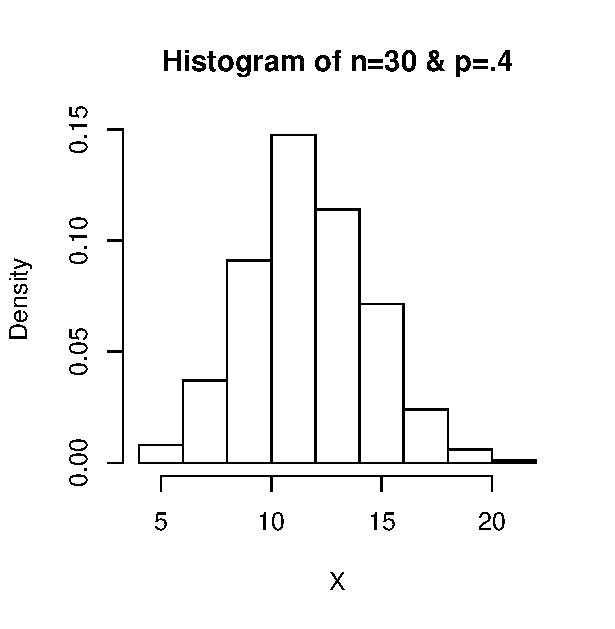
\includegraphics[width=8cm]{figure/LBL6a-1} 

}



\end{figure}

Therefore, like the binomial, the sampling distribution of $\hat{p}$ may be approximated by a normal curve with the correct mean and SD.

\begin{minipage}[ht]{3cm}

% \vspace{-31mm}

\textbf{Example:}
\end{minipage}
\begin{minipage}[ht]{11cm}

\parbox{11cm}{Toss a fair coin 50-times.  What is the chance of getting 60\% or more heads?
}
\end{minipage}

\begin{minipage}[ht]{3cm}

\vspace{-28mm}

\textbf{Solution:}
\end{minipage}
\begin{minipage}[ht]{11cm}

\parbox{11cm}{
The question is equivalent to `What is the probability that$\hat{p}$ exceed 0.60?'  Using the mean and SD given in the formula above with $n = 50$ and $p = 0.50$, the sample proportion is expected to be around 0.50 give or take $\sqrt{\frac{0.5 (0.5)}{50}}$ or 0.50 give or take 0.07.  With a mean of 0.50 and a SD 0.07, the area to the right of 0.60 (under the normal curve with mean 0.50 and SD 0.07) is 0.0766.  Thus, the proportion of heads will exceed 0.60 fewer than 8 percent of the time.

}
\end{minipage}

\begin{minipage}[ht]{3cm}

\vspace{-14mm}

\textbf{Example 3}
\end{minipage}
\begin{minipage}[ht]{11cm}

\parbox{11cm}{
If Best Buy sold 1200 smart watches last year, the percentage of smart watches sold with extended protection plans is expected to be around 20\%, give or take \underline{\phantom{xxxxxx}}.  Estimate the likelihood that it sold protection plans with more than 25\% of those watches.
}
\end{minipage}

\section{Estimating the Population Proportion p}

The Best Buy computations in the previous section assume that we know the protection plan sales rate is $p = 0.20$.  In data analysis, population parameters like $p$ are typically unknown and estimated from the data.  Consider estimating the proportion p of the current WMU graduating class who plan to go to graduate school.  Suppose we take a sample of 40 graduating students and suppose that 6 out of the 40 are planning to go to graduate school.  Then our estimate is $\hat{p} = \frac{6}{40} = 0.15$ of the graduating class plan to go to graduate school.  Now $\hat{p}$ is based on a sample, and unless we got really lucky, chances are the 0.15 estimate missed.  By how much?  On the average, a random variable misses the mean by one SD.  From the previous section, the SD of $\hat{p}$  equals $\sqrt{ \frac{pq}{n}}$.   It follows that the expected size of the miss is $\sqrt{ \frac{pq}{n}}$.   This last term is the \textit{standard error of estimation of the sample proportion}, or simply \textbf{standard error (SE)} of the proportion.

However, since we don't know $p$, we cannot calculate this SE.  In a situation like this, statisticians replace $p$ with $\hat{p}$  when calculating the SE.  The resulting quantity is called the \textit{estimated standard error of the sample proportion}.  In practice, however, the word ``estimated'' is dropped and estimated SE is simply called the SE.

\fbox{\parbox{14cm}{The population $p$ is \textbf{estimated using the sample proportion $\hat{p}$}.  This estimate tends to miss by an amount called the \textbf{standard error (SE)} of $\hat{p}$.
}}

\begin{equation*}
SE_{\hat{p}} = \sqrt{\frac{pq}{n}}
\end{equation*}

\begin{minipage}[ht]{3cm}

\vspace{-40mm}

\textbf{Exercise 4}
\end{minipage}
\begin{minipage}[ht]{11cm}

\parbox{11cm}{

Fill in the following blanks.

\begin{enumerate}
\item If 6 out of 40 students plan to go to graduate school, the proportion of all students who plan to go to graduate school is estimated as \underline{\phantom{xxxxxxx}}.  The standard error of this estimate is \underline{\phantom{xxxxxxx}}.
\item If 54 out of 360 students plan to go to graduate school, the proportion of all students who plan to go to graduate school is estimated as \underline{\phantom{xxxxxxx}}.  The standard error of this estimate is \underline{\phantom{xxxxxxx}}.
\end{enumerate}

}
\end{minipage}

Exercise 4 shows the effect of increasing the sample size on the SE of the sample proportion.  Multiplying the sample size by a factor of 9 (from 40 to 360) makes the SE decrease by a factor of 3.  In the formula for the SE of $\hat{p}$,  the sample size appears (i) in the denominator, and (ii) inside a square root.  Therefore, multiplying the sample size by a certain factor divides the SE of $\hat{p}$ by the square root of that factor.

\fbox{\parbox{14cm}{As the sample size $n$ \textbf{increases}, the $SE_{\hat{p}}$ \textbf{decreases} like the square root of the sample size.
}}

\section{Estimating Population Proportion Using Intervals}

Variables tend to miss their expected value but should be within \textit{one} SD 68\% of the time, and within 1.96 SD 95\% of the time.  Since the SE of $\hat{p}$ is simply an estimate of the SD, then we can write $| \hat{p} - p | \le 1.96(SE)$ or that $p$ is inside the interval $\hat{p} \pm 1.96(SE)$ 95\% of the time.  In other words, the interval $\hat{p} \pm 1.96(SE)$ contains the true value of $p$ with 95\% certainty.  This gives us an interval estimate for $p$.

\fbox{\parbox{14cm}{ \textbf{95\% Confidence Interval for p:} \\ A 95\% confidence interval estimate for the population proportion $p$ is given by

\begin{equation*}
  \hat{p} \pm 1.96 \sqrt{\frac{\hat{p} \hat{q}}{n}}
\end{equation*}

}}

The term $1.96 \sqrt{\frac{\hat{p} \hat{q}}{n}}$ is called the 95\% margin of error.

\begin{minipage}[ht]{3cm}

\vspace{-50mm}

\textbf{Exercise 5}
\end{minipage}
\begin{minipage}[ht]{11cm}

\parbox{11cm}{
Try the following problems.

\begin{enumerate}
\item If 6 out of 40 students plan to go to graduate school, the proportion of all students who plan to go to graduate school is estimated as \underline{\phantom{xxxxxxxxxx}}.  The margin of error is \underline{\phantom{xxxxxxxxxx}}.
\item Calculate a 95\% confidence interval estimate for the true proportion p of WMU students who plan to go to graduate school.
\item If 54 out of 360 students plan to go to graduate school, calculate a 95\% confidence interval estimate for the true proportion p of WMU students who plan to go to graduate school.
\end{enumerate}
}
\end{minipage}

\section{Sample Size for Estimating the Population Proportion}

If 9 out of 25 randomly selected WMU students live in Southwest Michigan, the 95\% confidence interval for the true proportion is $\hat{p} \pm 1.96 \sqrt{\frac{\hat{p} \hat{q}}{n}} = 0.36 \pm 0.19$.  This result says that the true proportion can be as low as 0.17 or as high as 0.55.  If we wanted to reduce the margin of error from 0.19 to some value $M$, then we set the formula for margin of error equal to $M$, i.e. $M = 1.96 \sqrt{\frac{\hat{p} \hat{q}}{n}}$.  Solving for $n$ gives the result we need.

\fbox{\parbox{14cm}{
To be 95\% confident that the sample proportion is within a distance $M$ of the true proportion $p$, choose a sample size equal to

\begin{equation*}
 n = (1.96)^2 \frac{ \hat{p} \hat{q}}{M^2}
\end{equation*}

where $\hat{p}$ is an estimate based on historical data or a pilot study.  The quantity $M$ is called the 95\% margin of error for $p$.

}}

\subsubsection{Example:} Suppose we want to reduce the margin of error for estimating the population proportion from 0.19 to 0.10.  Using the estimate $\hat{p} = 0.36$  based on the initial sample, the sample size we need is: $
n = (1.96)^2 \frac{(0.36)(0.64)}{0.10^2} = 89.$  To verify that this is the correct sample size, the 95\% confidence interval would be computed (if the sample proportion remained at 0.36) as $ 0.36 \pm (1.96)^2 \frac{(0.36)(0.64)}{(0.10)^2} = 89$.  To verify that this is the correct sample size, the 95\% confidence interval would be computed (if the sample proportion remained at 0.36) as $0.36 \pm (1.96) \sqrt{ \frac{0.36(0.64)}{89}} = 0.36 \pm 0.10$.

% \pagebreak
\twocolumn
\section{Exercises}
\begin{exercises}

\begin{exercise} % 1

Suppose that 20\% of students in a large university are graduate students.  If a random sample of 125 students are randomly selected, what is the probability that 25\% or more of the sample are graduate students?
\end{exercise}
\begin{solution} % 1


$P[ X \ge 32 ] = 0.0760321
\end{solution}

\begin{exercise} % 2

A sample of 100 observa- \\ tions is taken with 20 successes.

\begin{enumerate}
\item What is the estimate of the population proportion?
\item What is the standard error of this \\ estimate?
\item What is the 95\% margin of error?
\item What is the 95\% confidence interval?
\end{enumerate}

\end{exercise}
\begin{solution} % 2


\begin{enumerate}
\item The estimate of the population proportion is 0.2
\item The standard error of this estimate is 0.04
\item The 95\% margin of error is 0.0784
\item The 95\% confidence interval is $0.2 \pm 0.0784$
\end{enumerate}
\end{solution}

\begin{exercise} % 3

A sample of 100 individuals \\ showed that 20\% experienced gastrointestinal \\ problems  after consuming 10 grams of sorbitol, a common artificial sweetener.  Attach a standard error to this estimate.
\end{exercise}
\begin{solution} % 3


The standard error of this estimate is 0.04

\end{solution}

\begin{exercise} % 4

When a flight experiences fewer no-shows than expected, some passengers are \\ `bumped' from their flights (are denied boarding).  These incidents can reflect poorly on customer satisfaction.  Suppose United Airlines (for example) would like to estimate the true proportion of involuntarily bumped passengers across all domestic flights in the industry.  In a pilot study of 500 domestic passengers, 33 were involuntarily bumped.

\begin{enumerate}
\item	What is the estimate of the population proportion?
\item	What is the standard error of this \\ estimate?
\item	What is the 95\% margin of error?
\item	What is the 95\% confidence interval?
\end{enumerate}
\end{exercise}
\begin{solution} % 4


\begin{enumerate}
\item	The estimate of the population proportion is \\ $\hat{p} = 0.066$
\item	The standard error of this estimate is \\ $SE_{\hat{p}} = 0.0111035$
\item	The 95\% margin of error is $M_{\hat{p}} = 0.0217629$
\item	The 95\% confidence interval is \\ $0.066 \pm 0.0217629$
\end{enumerate}
\end{solution}

\begin{exercise} % 5

An appliance manufacturer offers maintenance contracts on its major appliances.  A manager wants to know what fraction of buyers of the company's convection ovens are also buying the maintenance contract with the oven.  From a random sample of 120 sales slips, 31 of the oven buyers opted for the contract.

\begin{enumerate}
\item	The proportion of customers who buy the contract along with their oven is estimated as \underline{\phantom{xxxxxxxxxx}}.
\item	Calculate a standard error for the estimate in (a).
\item	Calculate a 95\% confidence interval estimate for the true proportion of customers who buy the contract along with their oven.
\end{enumerate}
\end{exercise}
\begin{solution} % 5


\begin{enumerate}
\item	The estimate of the population proportion is \\ $\hat{p} = 0.2583333$
\item	The standard error of this estimate is \\ $SE_{\hat{p}} = 0.039958$
\item	The 95\% confidence interval is \\ $0.2583333 \pm 0.0783177$
\end{enumerate}
\end{solution}

\begin{exercise} % 6

Wiley Publications has determined that out of a sample of 5,511 of its publications for 2012, 1,754 of them are pirated in some form.

\begin{enumerate}
\item	What is the estimate of the population proportion?
\item	What is the standard error of this \\ estimate?
\item	What is the 95\% margin of error?
\item	What is the 95\% confidence interval?
\end{enumerate}
\end{exercise}
\begin{solution} % 6


\begin{enumerate}
\item	The estimate of the population proportion is \\ $\hat{p} = 0.3182725$
\item	The standard error of this estimate is \\ $SE_{\hat{p}} = 0.0062747$
\item The margin of error the estimate is \\ $M_{\hat{p}} = 0.0122983$
\item	The 95\% confidence interval is \\ $0.3182725 \pm 0.0122983$
\end{enumerate}
\end{solution}

\begin{exercise} % 7

Researchers who were \\ concerned if doctors were consistently adjusting dosages for weight of elderly patients studied 2000 prescriptions.  They found that for 600 of the  prescriptions, the doctors failed to adjust the \\ dosages.

\begin{enumerate}
\item	Doctors fail to adjust dosage for an estimated \underline{\phantom{xxxxxxxx}}  percent of prescriptions.
\item	Calculate a standard error for the percentage in (a).
\item	Calculate a 95\% margin of error for the percentage in (a).
\item	Calculate a 95\% interval estimate for the true proportion
\item	Calculate a 95\% confidence interval for the true percentage of prescriptions  \\ where doctors fail to adjust dosages.
\end{enumerate}
\end{exercise}
\begin{solution} % 7


\begin{enumerate}
\item	The estimate of the population proportion is \\ $\hat{p} = 0.3$
\item	The standard error of this estimate is \\ $SE_{\hat{p}} = 0.010247$
\item The margin of error the estimate is \\ $M_{\hat{p}} = 0.020084$
\item	The 95\% confidence interval is \\ $0.3 \pm 0.020084$
\item	The 95\% confidence interval is \\ $0.3 \pm 0.020084$
\end{enumerate}
\end{solution}


\end{exercises}
\onecolumn


%!Rnw root = ../../Master.Rnw

\chapter{Comparing Two Proportions }
\label{chap:ch9}

\section{Objective}

After completing this part, students should be able to:

\fbox{\parbox{14cm}{
\begin{itemize}
\item Explain the logic of estimation and the role of the sample, sampling
distribution and the population.
\item Make and interpret intervals for sample means and sample proportions.
\item Describe the relationships between trust levels, sample size, and the width
of the confidence interval.  \index{confidence interval}
\end{itemize}

}}

\section{Estimating the difference between independent proportions}

Has retention rate at WMU changed over time?  Suppose that a random sample of 200 entering students in 1989 showed 74\% were still enrolled 3 years later.  Another random sample of 200 entering students in 1999 showed that 66\% were still enrolled 3 years later.  This constitutes an 8\% change in 3-year retention rate.  However, the 8\% difference is based on random sampling, and is only an estimate of the true difference.  What is the likely size of the error of estimation?

Changing notation from percentage to proportions and taking the difference of
0.74 - 0.66, we get 0.08 to compare retention rates.  The proportions of 0.74 and 0.66 are \textit{independent} proportions, in the sense that they are based on separate and independent groups of students.  The SE of the difference is

\begin{equation*}
  SE_{(\hat{p}_1 - \hat{p}_2)} = \sqrt{ SE_{\hat{p}_1}^2 + SE_{\hat{p}_2}^2}
\end{equation*}

Whenever the two proportions are independent.  Applying equation SE of $\hat{p} = \sqrt{ \frac{ \hat{p} \hat{q} }{n}}$ twice, we have $SE_{\hat{p}_1} = \sqrt{ \frac{ \hat{p}_1 \hat{q}_1 }{n_1}}$ and $SE_{\hat{p}_2} = \sqrt{ \frac{ \hat{p}_2 \hat{q}_2 }{n_2}}$.  Substituting into the formula above, $SE_{(\hat{p}_1 - \hat{p}_2)} = \sqrt{ SE_{\hat{p}_1}^2 + SE_{\hat{p}_2}^2}$, we get:

\fbox{\parbox{14cm}{
\textbf{Standard Error of the Difference between two independent Proportions}

\begin{equation*}
  SE_{( \hat{p}_1 - \hat{p}_2)} = \sqrt{ \frac{ \hat{p}_1 \hat{q}_1}{n_1} + \frac{ \hat{p}_2 \hat{q}_2}{n_2}}
\end{equation*}
}}

Continuing with the retention rate example, we let $\hat{p}_1 = 0.74$, $\hat{p}_2 = 0.66$, $n_1 = 200$, $n_2 = 200$ so that

$$ SE_{( \hat{p}_1 - \hat{p}_2)} = \sqrt{ \frac{ 0.74 (0.26)}{200} + \frac{ 0.66 (0.34) }{200}} = 0.045 $$

Thus, the difference in retention rate is estimated by $0.74 - 0.66 = 0.08$ with a standard error of 0.045.  Changing notation back to a percentage and with less technical language, the drop-in retention rate is estimated to be 8\%, give or take 4.5\% or so. We also could have computed $ SE_{( \hat{p}_1 - \hat{p}_2)}$  in three steps.  First by using $SE_{\hat{p}}$ twice,

\begin{equation*}
  SE_{\hat{p}_1} = \sqrt{ \frac{\hat{p}_1 \hat{q}_1}{n_1}} = \sqrt{ \frac{0.74  (0.26)}{200}} = 0.031
\end{equation*}

\begin{equation*}
  SE_{\hat{p}_2} = \sqrt{ \frac{\hat{p}_2 \hat{q}_2}{n_2}} = \sqrt{ \frac{0.66  (0.34)}{200}} = 0.033
\end{equation*}

Then using $ SE_{( \hat{p}_1 - \hat{p}_2)} = \sqrt{ SE_{\hat{p}_1}^2 + SE_{\hat{p}_1}^2} = \sqrt{ (0.031)^2 + (0.033)^2} = 0.045 $

\subsection{Using a confidence interval}

The difference of two proportions is a random variable with expected value and spread.  The 68\% and 95\% rules apply, i.e.  the estimated difference $\hat{p}_1 - \hat{p}_2$ should be close to the true value -- within \textit{one} SE 68\% of the time, and within 1.96 SE's 95\% of the time.  Following the same reasoning as before,

\begin{equation*}
  (\hat{p}_1 - \hat{p}_2) \pm 1.96 (SE_{(\hat{p}_1 - \hat{p}_2)})
\end{equation*}

should contain the true difference $p_1 - p_2$ with 95\% level of confidence.  Substituting
$$ SE_{( \hat{p}_1 - \hat{p}_2)} = \sqrt{ \frac{ \hat{p}_1 \hat{q}_1}{n_1} + \frac{ \hat{p}_2 \hat{q}_2}{n_2}} $$,
we get the following formula:

\begin{center}
\fbox{\parbox{14cm}{
\textbf{95\% Confidence Interval for $p_1 - p_2$}

\begin{equation*}
  ( \hat{p}_1 - \hat{p}_2) \pm 1.96 \sqrt{ \frac{ \hat{p}_1 \hat{q}_1}{n_1} + \frac{ \hat{p}_2 \hat{q}_2}{n_2}}
\end{equation*}
}}
\end{center}

For retention rate, the difference between 1989 and 1999 was estimated as 0.08 with SE = 0.045.  Therefore, a 95\% confidence interval for the change is

\begin{equation*}
0.08 \pm 1.96 (0.045)
\end{equation*}

or $0.08 \pm 0.088 = (-0.008, 0.168)$.  Rounding off to $(-0.01, 0.17)$, we say that the drop-in retention rate from 1989 to 1999 is between $-0.01 \texttt{ and } 0.17$ with 95\% confidence. Note that \textbf{zero} is contained or is not been excluded from the interval, making it still a possibility that there is no real change in retention rate, just chance variability.

\section{Statistical significance}

Let $\hat{p}_1$ be the proportion of heads in 50 tosses of a coin.  Let $\hat{p}_2$  be the proportion of heads in the next 50 tosses of the same coin.  Will $\hat{p}_1$  and $\hat{p}_1$ be equal?  Not likely.  They will tend to differ, due to ``luck of the draw'' or chance variability.

The table below shows partial data from an occupation survey by the Census Bureau. In this 2009 survey, regular `cooks' were a separate classification from `chefs or head cooks.'  Note that even though 37\% of cooks were women, only 16\% of chefs or head cooks were women.  Is the difference just luck of the draw, or due to something else besides chance?

\begin{table}[ht]
\centering
\begin{tabular}{@{} cccc @{}} \hline
       & Women & Men & Total \\ \hline
Cooks & 441 & 762 & 1203 \\
Chefs or Head Cooks & 45 & 245 & 290 \\ \hline
\end{tabular}
\end{table}

Statistics helps decision-making in cases like these by assessing how much chance variability to expect between two proportions.  Following the calculations of section above, we have

\begin{equation*}
  \hat{p}_1 - \hat{p}_2 = \frac{441}{1203} - \frac{45}{290} = 0.37 - 0.16 = 0.21
\end{equation*}

with a standard error

\begin{equation*}
  SE_{(\hat{p}_1 - \hat{p}_2)} = \sqrt{ \frac{0.37(0.63)}{1203} + \frac{0.16(0.84}{290}} = 0.026
\end{equation*}

The 95\% confidence interval for $p_1 - p_2$ is

\begin{equation*}
0.21 \pm 1.96 (0.026) = (0.16, 0.26)
\end{equation*}

Thus, even allowing for 1.96 SE's of chance variability, the true difference between proportions is at least 0.16 (and could be as large as 0.26).  This means that the interval does not contain or it excluded 0 from the range of possible values.  When this happens, statisticians say that the differences are \textit{statistically significant}.

\fbox{\parbox{14cm}{
If the confidence interval for $\hat{p}_1 - \hat{p}_2$ excludes \textbf{zero}, then the difference is \textbf{statistically significant.}

}}

\subsection{The P-value}

For convenience, let us continue the example of the previous section.

\begin{minipage}[ht]{3cm}

\vspace{-4mm}

\textbf{Question}
\end{minipage}
\begin{minipage}[ht]{12cm}

\parbox{12cm}{
If chance alone was at work, how likely will we get a difference of 0.21 between two proportions?
}
\end{minipage}

\begin{minipage}[ht]{3cm}

\vspace{-3mm}

\textbf{Answer}
\end{minipage}
\begin{minipage}[ht]{12cm}

\parbox{12cm}{
Very small, less than 0.0001 (or 1 in 10,000).
}
\end{minipage}

The `likelihood of getting 0.21 by chance' is called a P-value. The fact that it is very small means we should exclude the option that `chance alone is at work.'

The actual probability calculation is beyond the scope of this class.  Let's just say that random variables very rarely go past 4 SE's from their expected values (less than 1 in 10,000 times).  Since the SE for the difference is 0.026, the observed difference $\hat{p}_1 - \hat{p}_2 = 0.21$  is not just 1, nor 2, but 8 SE's from 0.  This cannot be just chance alone.   Something else is at work.

\begin{center}
\fbox{\parbox{12cm}{
\textbf{The Rule for $p$-value:} \\
If the $p$-value $\le 0.05$, the difference is \textit{statistically significant.} \\
If the $p$-value $\le 0.01$, the difference is called \textit{highly significant.}
}}
\end{center}

In the occupation example, we can say that the percentage of women head chefs
is lower than that of regular cooks.  Furthermore, the difference is highly significant.

\subsection{Risk ratio and odds ratio}   %%%%%%%%%%%%%%

 In clinical studies, statisticians frequently take ratios of proportions or probabilities (instead of differences).  There are several reasons for this idea.  Sometimes, the disease or medical event of interest is quite rare, i.e., $p_1 = 0.0008$.  If a new treatment reduces the probability of getting the disease to 0.0006, the difference in probabilities is quite small and hard to assess $((p_1 - p_2) = 0.0002)$.  In the meantime, the ratio $ \frac{p_2}{p_1} = \frac{0.0006}{0.0008} = 0.75 $ means that the risk of getting the disease under the new treatment has been reduced by 25\%.

A second reason for taking ratios is more technical.  The ratio can more easily be adjusted to control for other variables like age and race.

 \subsection{Risk ratio}

Following is the abstract of the study ``Safety and Efficacy of a Recombinant Hepatitis E Vaccine.''  % \citep{shrestha2007}

\subsubsection{Background}

Hepatitis E virus (HEV) is an important cause of viral hepatitis.  We evaluated
the safety and efficacy of an HEV recombinant protein (rHEV) vaccine in a phase
2, randomized, double-blind, placebo-controlled trial.

\subsubsection{Methods}

In Nepal, we studied 2000 healthy adults susceptible to HEV infection who were randomly assigned to receive three doses of either the rHEV vaccine or placebo at months 0, 1, and 6. Active (including hospital) surveillance was used to identify acute hepatitis and adverse events. The primary end point was the development of hepatitis E after three vaccine doses.

\subsubsection{Results}

A total of 1794 subjects (898 in the vaccine group and 896 in the placebo group) received three vaccine doses; the total vaccinated cohort was followed for a median of 804 days.  After three vaccine doses, hepatitis E developed in 69 subjects, of whom 66 were in the placebo group.  The vaccine efficacy was 95.5\% (95\% confidence interval [CI], 85.6 to 98.6).  In an intention-to-treat analysis that included all 87 subjects in whom hepatitis E developed after the first vaccine dose, 9 subjects were in the vaccine group, with a vaccine efficacy of 88.5\% (95\% CI, 77.1 to 94.2).  Among subjects in a sub-group randomly selected for analysis of injection-site findings and general symptoms (reactogenicity sub-group) during the 8-day period after the administration of any dose, the proportion of subjects with adverse events was similar in the two study groups, except that injection-site pain was increased in the vaccine group ($p = 0.03$).

\subsubsection{Conclusion}

In a high-risk population, the rHEV vaccine was effective in the prevention of
hepatitis E.

The data given in the `Results' part of the abstract may be summarized as follows.

\begin{table}[ht]
\centering
\begin{tabular}{@{} cccc @{}} \hline
 & \multicolumn{2}{c}{hepatitis E} \\
 & Yes & No & Total \\ \hline
 Vaccine & 3 & 895 & 898 \\
 Placbo  & 66 & 830 & 896 \\ \hline
 \end{tabular}
 \end{table}

We may present data for comparing proportions in a 2 by 2 table.

\begin{table}[ht]
\centering
\begin{tabular}{@{} cccc @{}} \hline
 & \multicolumn{2}{c}{Disease} \\
 & Yes & No & Total \\ \hline
 Exposure & a & b & $a + b$ \\
 No Exposure  & c & d & $c + d$ \\ \hline
 \end{tabular}
 \end{table}

The risk ratio, also called the relative risk is the ratio of probabilities

\begin{equation*}
  RR = \frac{ \frac{P(Disease)}{Exposure}}{ \frac{P(Disease)}{No Exposure} } = \frac{ \frac{a}{a + b}}{ \frac{c}{c + d} } = \frac{p_1}{p_2}
\end{equation*}

For our example, we can define and calculate the risk ratio as

\begin{equation*}
  RR = \frac{ \frac{P(Disease)}{Exposure}}{ \frac{P(Disease)}{No Exposure} } = \frac{ \frac{3}{898}}{ \frac{66}{896} } = \frac{0.00334}{0.07366} = 0.045
\end{equation*}

This means that getting the vaccine reduces your risk to only 4.5\% of the original, or has 95.5\% efficacy.

\subsection{A 95\% confidence interval for risk ratio}

Confidence interval formulas are generally written for the natural logarithm of RR.  Consider a 2 by 2 table as before.

\begin{table}[ht]
\centering
\begin{tabular}{@{} cccc @{}} \hline
 & \multicolumn{2}{c}{Disease} \\
 & Yes & No & Total \\ \hline
 Exposure & a & b & $a + b$ \\
 No Exposure  & c & d & $c + d$ \\ \hline
 \end{tabular}
 \end{table}

We will calculate the confidence interval for RR in 4 steps.

\begin{enumerate}
\item Calculate the \textbf{natural log (ln)} of the risk ratio:
$$ ln(RR) = ln \left( \frac{ \frac{a}{a + b}}{ \frac{c}{c + d} } \right) $$

\item Calculate the standard error of ln(RR) as follows:

\begin{equation*}
   SE_{ln(RR)} = \sqrt{ \frac{1}{a} + \frac{1}{c} - \frac{1}{a + b} - \frac{1}{c + d}}
\end{equation*}

\item A 95\% confidence interval for ln(RR) is given by

\begin{equation*}
  [ ln(RR) - 1.96 (SE), ln(RR) + 1.96 (SE) ]
\end{equation*}

\item Finally, a 95\% confidence interval for RR is given by

\begin{equation*}
  \Big[ e^{ln(RR) - 1.96 (SE)}, e^{ln(RR) + 1.96 (SE)} \Big]
\end{equation*}

\end{enumerate}

Returning to our example,

\begin{enumerate}
\item
\begin{equation*}
ln(RR) = ln(0.045) = -3.101
\end{equation*}

\item
\begin{equation*}
SE = \sqrt{ \frac{1}{3} + \frac{1}{66} - \frac{1}{898} - \frac{1}{896}} = \sqrt{0.3462} = 0.5884
\end{equation*}

\item
\begin{equation*}
 [ -3.101 - 1.96(0.5884), -3.101 + 1.96(0.5884) ] = [ -4.254, 1.948]
\end{equation*}

\item
\begin{equation*}
  \Big[ e^{-4.254}, e^{-1.948} \Big] = [ 0.014, 0.143 ]
\end{equation*}

\end{enumerate}

With 95\% confidence, the risk of getting hepatitis with the vaccine is only 1.4\% to 14.3\% of placebo.  This means that the vaccine reduces your risk by as low as 85.7\% or as high as 98.6\%.  Now read the Results section of the abstract again.  They say ``The vaccine efficacy was 95.5\% (95\% confidence interval [CI], 85.6 to 98.6).''  The two sets of numbers match, (slight discrepancy due to rounding error.)

\subsection{Odds ratio}

The odds of an event occurring is

\begin{equation*}
  Odds = \frac{ \texttt{Probability that event occurs}}{\texttt{Probability that event doesn't occur}} = \frac{p}{q}
\end{equation*}

For example, if you win a game a 20\% of the time ($p = 0.20$), then your odds of winning is $( \frac{0.20}{0.80}) = \frac{1}{4}$.  We say that you have a \textit{1-in-4} odds of winning, or you win once for every 4 times you lose.  If you win 80\% of the time, the odds are $\frac{0.80}{0.20} = 4$. This means you have \textit{4-in-1} odds of winning, or you win 4 times for every one time you lose.  Here is a table of odds corresponding to various probabilities.

\begin{table}[ht]
\centering
\begin{tabular}{@{} cc @{}} \hline
Probability & Odds \\ \hline
0.10 & 1/9 = 0.11 \\
0.20 & 1/4 = 0.25 \\
0.50 & 1/1 = 1.00 \\
0.80 & 4/1 = 4.00 \\
0.90 & 9/1 = 9.00 \\ \hline
\end{tabular}
\end{table}

Unlike probabilities, odds can be bigger than 1.  The odds ratio is simply the ratio of two odds (usually for comparing two groups).

\begin{equation*}
  Odds Ratio = \frac{ \texttt{Odds of Group 1}}{\texttt{Odds of Group 2}} = \frac{ \frac{p_1}{q_1}}{ \frac{p_2}{q_2}}
\end{equation*}

Returning to the hepatitis E study, recall the disease occurrence data:

\begin{table}[ht]
\centering
\begin{tabular}{@{} cccc @{}} \hline
 & \multicolumn{2}{c}{hepatitis E} \\
 & Yes & No & Total \\ \hline
 Vaccine & 3 & 895 & 898 \\
 Placbo  & 66 & 830 & 896 \\ \hline
 \end{tabular}
 \end{table}

The disease rate for each group is

\begin{equation*}
  \texttt{Odds(Hepatitis|Placebo)} = \frac{0.07366}{(1-0.07366)} = 0.07952
\end{equation*}

\begin{equation*}
  \texttt{Odds(Hepatitis|Vaccine)} = \frac{0.00334}{(1-0.00334)} = 0.00335
\end{equation*}

\begin{equation*}
  \texttt{Odds Ratio} = \frac{\texttt{Odds(Hepatitis|Placebo)}}{\texttt{Odds(Hepatitis|Vaccine)}} = \frac{0.07952}{0.00335} = 23.7
\end{equation*}

We say that ``the odds of getting hepatitis is 24 times greater if you remain unvaccinated.''

Odds ratios are generally easier to interpret if they are larger than one.  We can always ensure this by choosing which group to put in the numerator, i.e., the one with larger odds.

It is important to understand that the odds ratio is not a ratio of likelihood or probabilities.  If the disease rates for men and women are 0.80 and 0.40, respectively, then the odds ratio is

\begin{equation*}
   \frac{ \frac{0.80}{0.20}}{ \frac{0.40}{0.60}} = 6.00
\end{equation*}

In this example, men are twice as likely to get the disease, but have 6 times the odds.

\subsection{A 95\% confidence interval for odds ratio}

Confidence interval formulas for odds ratios (OR) are generally written for the natural logarithm, similarly to risk ratios.  Consider a 2 by 2 table as before.

\begin{table}[ht]
\centering
\begin{tabular}{@{} cccc @{}} \hline
 & \multicolumn{2}{c}{Disease} \\
 & Yes & No & Total \\ \hline
 Exposure & a & b & $a + b$ \\
 No Exposure  & c & d & $c + d$ \\ \hline
 \end{tabular}
 \end{table}

The odds of disease occurrence in the exposed group is $\Big[ \frac{ \frac{a}{a + b}}{ \frac{b}{a + b}} \Big] = \frac{a}{b} $.  Similarly, the odds in the unexposed group is $\frac{c}{d}$.  Hence, the odds ratio of disease occurrence is

\begin{equation*}
  \texttt{OR} = \frac{\texttt{Odds(Disease|Exposed)}}{\texttt{Odds(Disease|Not Exposed)}} = \frac{a/b}{c/d} = \frac{p_1 / q_1}{p_2 / q_2} = \frac{ p_1 \times (1- p_2)}{ p_2 \times (1 - p_1)}
\end{equation*}

If $OR < 1$, we can put the `not exposed' group in the numerator, so that $OR > 1$  (the resulting odds ratio should, of course, be interpreted accordingly).  In our hepatitis example, we can use the following table:

\begin{table}[ht]
\centering
\begin{tabular}{@{} cccc @{}} \hline
 & \multicolumn{2}{c}{hepatitis E} \\
 & Yes & No & Total \\ \hline
 Placbo  & 66 & 830 & 896 \\
 Vaccine & 3 & 895 & 898 \\
  \hline
 \end{tabular}
 \end{table}

and get $OR = (66)(895)/(830)(3) = 23.7$ (``Placebo group has 24 times the odds of getting hepatitis''). If we use

\begin{table}[ht]
\centering
\begin{tabular}{@{} cccc @{}} \hline
 & \multicolumn{2}{c}{hepatitis E} \\
 & Yes & No & Total \\ \hline
 Vaccine & 3 & 895 & 898 \\
 Placbo  & 66 & 830 & 896 \\
  \hline
 \end{tabular}
 \end{table}

then $OR = (3)(830)/(66)(895) = 0.04$ (``Vaccine group has 0.04 times the odds of getting hepatitis'').

In either case, we will calculate the confidence interval for odds ratio in 4 steps.

\begin{enumerate}
\item Calculate the natural log of the odds ratio:
\begin{equation*}
  ln(OR) = ln \Big( \frac{a \times d}{b \times c} \Big)
\end{equation*}

\item	Calculate the standard error of ln(OR) as follows:
\begin{equation*}
  SE_{ln(OR)} = \sqrt{ \Big( \frac{1}{a} + \frac{1}{b} + \frac{1}{c} + \frac{1}{d} \Big)}
\end{equation*}

\item A 95\% confidence interval for ln(OR) is given by
\begin{equation*}
  [ ln(OR) - 1.96(SE), ln(OR) + 1.96(SE)]
\end{equation*}

\item Finally, a 95\% confidence interval for OR is given by
\begin{equation*}
   e^{ln(OR) - 1.96(SE)}, e^{ln(OR) + 1.96(SE)}
\end{equation*}

\end{enumerate}

Returning to the hepatitis E study, recall the disease occurrence data:

\begin{table}[ht]
\centering
\begin{tabular}{@{} cccc @{}} \hline
 & \multicolumn{2}{c}{hepatitis E} \\
 & Yes & No & Total \\ \hline
 Placbo  & 66 & 830 & 896 \\
 Vaccine & 3 & 895 & 898 \\
  \hline
 \end{tabular}
 \end{table}

The odds ratio of getting hepatitis is

\begin{equation*}
  \texttt{Odds Ratio} = \frac{\texttt{Odds(Hepatitis|Placebo)}}{\texttt{Odds(Hepatitis|Vaccine)}} = \frac{66 \times 895}{3 \times 830} = 23.7
\end{equation*}

so that

\begin{enumerate}
\item
\begin{equation*}
  ln(OR) = ln(23.7) = 3.165
\end{equation*}

\item
\begin{equation*}
  SE_{ln(OR)} = \sqrt{ \frac{1}{66} + \frac{1}{830} + \frac{1}{3} + \frac{1}{895}   } = \sqrt{0.3508} = 0.5923
\end{equation*}

\item
\begin{equation*}
 [3.165-1.96 (0.5923), 3.165+1.96 (.5923)] = [2.004, 4.326]
\end{equation*}

\item
\begin{equation*}
  [ e^{2.004}, e^{4.326} ]
\end{equation*}
\end{enumerate}

With 95\% confidence, the odds of unvaccinated subjects getting hepatitis is between 7 and 76 times greater than vaccinated subjects.

\section{Key Words}

\colorbox{lgray}{\parbox{14cm}{
\begin{minipage}[ht]{6cm}

\begin{itemize}
\item $\alpha$ (Alpha)
\item Bias
\item Confidence interval
\end{itemize}
\end{minipage} \hfill
\begin{minipage}[ht]{6cm}

\begin{itemize}
\item Confidence level
\item Efficiency
\item margin of error
\end{itemize}
\end{minipage}
}}


\twocolumn
\section{Exercises}
\begin{exercises}

  \begin{exercise}  % 1

In a study of drug usage by students at a large university, data was obtained regarding hard liquor experience of \\ smokers and  nonsmokers.

\begin{table}[ht]
\centering
\begin{tabular}{@{} cccc @{}} \hline
 & \multicolumn{2}{c}{Drug Use} \\
 & Once or more & Never & Total \\ \hline
Smokers & 23 & 18 & 41 \\
Nonsmokers & 15 & 56 & 71 \\ \hline
\end{tabular}
\end{table}

\begin{enumerate}
\item Estimate the difference in percentage of \\ drug use between smokers and nonsmokers.
\item Calculate a standard error for your estimate in (1).
\item Calculate a 95\% confidence interval for the difference in percentage of drug use \\ between smokers and nonsmokers.
\item Estimate the risk ratio of drug use \\ between smokers and nonsmokers.
\item Calculate a standard error for the natural log of your estimate in 4.
\item Calculate a 95\% confidence interval for the risk ratio of drug use between smokers
\item Estimate the odds ratio of drug use \\ between smokers and nonsmokers.
\item Calculate a standard error for the natural log of your estimate in 7.
\item Calculate a 95\% confidence interval for the odds ratio of drug use  between \\ smokers and nonsmokers.
\item Interpret the above confidence intervals in parts 3, 6, and 9. Which are significant, and which are not? Why or why not?
\end{enumerate}
  \end{exercise}
  \begin{solution}  % 1



\begin{enumerate}
\item The difference in percentage of  drug  use \\ between smokers and nonsmokers is 35.0.
\item Calculate a standard error for your estimate in (1).
\item Calculate a 95\% confidence interval for the difference in percentage of drug use \\ between smokers and nonsmokers.
\item Estimate the risk ratio of drug use \\ between smokers and nonsmokers.
\item Calculate a standard error for the natural log of your estimate in 4.
\item Calculate a 95\% confidence interval for the risk ratio of drug use between smokers
\item Estimate the odds ratio of drug use \\ between smokers and nonsmokers.
\item Calculate a standard error for the natural log of your estimate in 7.
\item Calculate a 95\% confidence interval for the odds ratio of drug use between smokers and nonsmokers.
\item Interpret the above confidence intervals in parts 3, 6, and 9. Which are significant, and which are not? Why or why not?
\end{enumerate}

  \end{solution}

  \begin{exercise} % 2

Time magazine reported the result of a telephone poll of 800 adult Americans. The question posed of the Americans who were surveyed was: ``Should the federal tax on cigarettes be raised to pay for health care reform?''

\begin{table}[ht]
\centering
\begin{tabular}{@{} lcc @{}} \hline
 & \multicolumn{2}{c}{Federal Tax} \\
  & \multicolumn{2}{c}{on Cigarettes} \\
Status & Yes & No \\ \hline
Smoker & 41 & 154 \\
Nonsmoker & 351 & 254 \\ \hline
\end{tabular}
\end{table}

	  \begin{enumerate}
	  \item Estimate the difference in percentage of Americans who supported the federal \\ tax on cigarettes between smokers and non-smokers.
    \item Calculate a standard error for your estimate in (1).
    \item Calculate a 95\% confidence interval for the difference in percentage of Americans who supported the federal tax on cigarettes between smokers and non- \\ smokers.
    \item Estimate the risk ratio of Americans \\ who supported the federal tax on \\ cigarettes between smokers and non- \\ smokers.
    \item Estimate the odds ratio of Americans who supported the federal tax on \\ cigarettes between smokers and non- \\ smokers.
	  \end{enumerate}

	\end{exercise}
	\begin{solution}  % 2

		  \begin{enumerate}
	  \item Estimate the difference in percentage of Americans who supported the federal tax on cigarettes between smokers and non-smokers.
    \item Calculate a standard error for your estimate in (1).
    \item Calculate a 95\% confidence interval for the difference in percentage of Americans who supported the federal tax on cigarettes between smokers and non-smokers.
    \item Estimate the risk ratio of Americans who supported the federal tax on cigarettes between smokers and non-smokers.
    \item Estimate the odds ratio of Americans who supported the federal tax on cigarettes between smokers and non-smokers.
	  \end{enumerate}

   	\end{solution}

  \begin{exercise} % 3

The age at which a woman gives birth to her first child may be an \\ important factor in the risk of later \\ developing breast cancer.  An international study conducted by WHO selected women \\ with at least one birth and recorded if they had breast cancer or not and whether they had their first child before their $30^{th}$ birthday or after. In a sample of 3220 women who had their first child after their $30^{th}$ birthday, 683 developed breast cancer.  Whereas, in a sample of 10245 women who had their first child before their $30^{th}$ birthday, 1483 developed breast cancer.

	  \begin{enumerate}
	  \item Estimate the difference in percentage \\ of developing breast cancer between \\ women who had their first child after their $30^{th}$ birthday and before their $30^{th}$ birthday.
    \item Calculate a standard error for your \\ estimate in (1).
    \item Calculate a 95\% confidence interval for the difference in percentage developing breast cancer between women who had their first child after their $30^{th}$ birthday and before their $30^{th}$ birthday.
    \item Estimate the risk ratio of developing \\ breast cancer between women who had their first child after their $30^{th}$ birthday and before their $30^{th}$ birthday.
    \item Estimate the odds ratio of developing \\ breast cancer between women who had their first child after their $30^{th}$ \\ birthday and before their $30^{th}$ \\ birthday.
	  \end{enumerate}
  \end{exercise}
  \begin{solution}  % 3

   The critical value is
[1] 1.984217

  \end{solution}

  \begin{exercise} % 4

In a sample of 200 surgeons, 15\% thought the government should control health care.  Whereas, in a sample of 200 gen- \\ eral practitioners, 21\% thought the same.

\begin{enumerate}
\item Estimate the difference in percentage of those who think the government should control health care between surgeons \\ and general practitioners.
\item Calculate a standard error for your \\ estimate in (1).
\item Calculate a 95\% confidence interval for the difference in percentage of those who \\ think the government should control \\ health care between surgeons and \\ general practitioners.
\item Estimate the risk ratio of those who \\ think the government should control \\ health care between surgeons and \\ general practitioners.
\item Estimate the odds ratio of those who \\ think the government should control \\ health care between surgeons and \\ general practitioners.
\end{enumerate}
  \end{exercise}
  % \begin{solution}  % 4
  %
  %     SE =
  %     <<results="asis", echo=FALSE>>=
  %       SE1 <- 0.3/sqrt(100)
  %       SE1
  %     @
  %
  %     ME =
  %     <<results="asis", echo=FALSE>>=
  %       ME1 <- CV1 * SE1
  %       ME1
  %     @
  % \end{solution}


\end{exercises}
\onecolumn


%!Rnw root = ../../Master.Rnw

\chapter{Sampling Distribution of the Mean}
\label{chap:ch10}

\section{Objectives}

After completing this part, students should be able to:

\fbox{\parbox{14cm}{

\begin{itemize}
\item Define and explain the concept of the {\textbf{distribution of the sample mean}}.
\item Convert empirical scores to z-scores and use z-scores and the Normal Distribution curve
table to find areas above, below and between points of the curve and  express them regarding their probabilities.
\item Utilize the standard normal distribution to solve probability (chance) problems.
\end{itemize}
}}

\section{Behavioral Properties of the Sample Average}

What percentage of adult men are between 5'6'' and 6' tall?  Population surveys have shown that men's heights are approximately normally distributed with mean 5'9'' and SD 3''.  Thus the percentage of men between 5'6'' and 6' is estimated as 68\%, the percentage within 1 SD of the mean.  See Figure 10.1 below.

\begin{figure}[ht]
\caption{The Percentage of Men's Heights between 66 and 72 inches}



{\centering 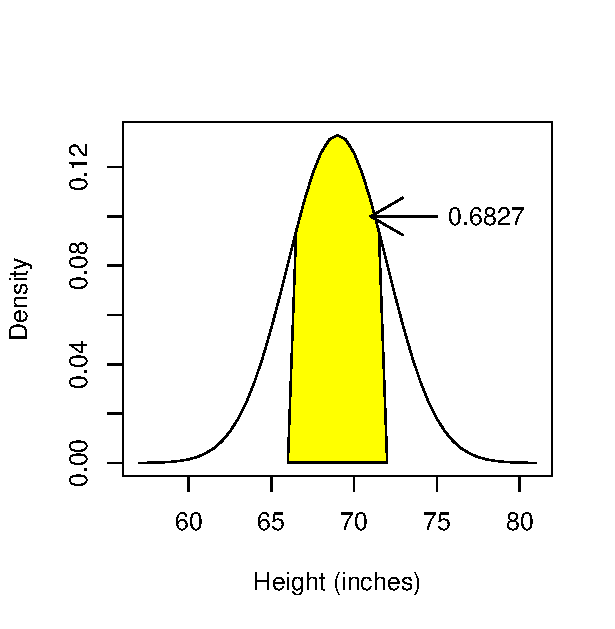
\includegraphics[width=6cm]{figure/LBL10-1} 

}




\end{figure}

If the population of men are randomly assigned into groups of 9, and the average heights are computed for each group, what percentage of groups average between 5'6'' and 6' in height?    Is the answer approximately 68\%?  No.  In fact, more than 99\% of the groups will average between 5'6'' and 6', even though only 68\% of individuals do.  Why?  Because averages tend to include tall, short and medium heights -- therefore averages tend to fall closer to middle than individuals.   (Think about this:  We put in a hat the names of all the men in class.  You will win \$20 if the names you draw average over 6 feet tall.  Would you rather draw 1 or 2 names?  What are your chances of winning if you draw 9 names?)  

The following is a small simulation study of the behavior of the sample mean.  Fifty samples are drawn (each containing $n = 9$ individuals) from a population with mean 69 inches and SD 3 inches.  For each sample, we calculate the average.  Observe that none of the samples average over 71 inches, even though many individuals do.

\begin{table}[ht]
\caption{Heights of 50 samples of Nine Men}
\begin{tabular}{@{} ccccccccccc @{}} \hline
Sample & (1)&(2)&(3)&(4)&(5)&(6)&(7)&(8)&(9)& Ave \\ \hline
1: &65.5&66.8&68.9&67.8&71.9&66.8&71.0&73.1&62.6&68.27 \\
2: &68.6&71.2&72.6&64.3&70.9&70.0&69.0&69.8&62.4&68.75 \\
3: &67.4&67.9&67.1&68.2&70.7&68.3&67.2&68.7&67.0&68.04 \\
$\vdots$ & $\vdots$ & $\vdots$ & $\vdots$ & $\vdots$ & $\vdots$ & $\vdots$ & $\vdots$ & $\vdots$ & $\vdots$ & $\vdots$ \\ \hline
SD: &3.17&2.56&2.66&3.25&2.94&2.56&3.10&3.33&3.62 & 0.92 \\
Mean: &68.53&68.18&68.92&68.51&69.26&68.72&68.66&68.86&68.11& 68.64 \\ \hline
\end{tabular}
\end{table}

The first lesson of this chapter says:

\fbox{\parbox{14cm}{Averages are less variable than individuals}}

Do you see this in the simulation study?  To make it easier to see, look at the SD of each column.  The SD of individuals tend to be around 3.0 (the true value), but the SD of averages is much smaller.  How much smaller?  We now state the main lesson of the chapter.

\fbox{\parbox{14cm}{SD of $\bar{X} = \frac{\texttt{SD of individuals}}{\sqrt{n} }$ }}

Since the individuals in the simulation study have SD of 3 inches, the SD of 9-member averages is:

\fbox{\parbox{14cm}{SD of $\bar{X}_{n=9} = \frac{\texttt{SD of individuals}}{\sqrt{n} } = \frac{3}{\sqrt{9}} = 1.0$ }}

Therefore, the true value for the SD of the last column is 1.0.  The simulated SD is 0.92, which is close.

\subsubsection{Example 1}

Suppose that men's heights are normally distributed with a mean 5'9'' and a SD 3''.
  
  \begin{enumerate}
  \item What percentage of men are over 5'11'' tall?
  \item Select a man at random.  What is the probability that he is over 5'11'' tall?
  \item If the average height were calculated for all possible samples of size 9 that can be taken, what percentage of averages will exceed 5'11''?
  \item Given one randomly selected sample of size 9, what is the probability that the average height will exceed 5'11''?
  \item Given a sample of size 25, what is the probability that the average height will exceed 5'11''?
  \item Given a sample of size 9, the average height of the sample will exceed \underline{\phantom{xxxxxxxx}} with probability 0.90
  \item 90\% of samples of size 9 will have average height exceeding \underline{\phantom{xxxxxxxx}}.
  \end{enumerate}

\section{Estimating the Population Mean}

Consider estimating the average GPA (call this $\mu$) of the approximately 23,000 WMU undergraduates.  In the absence of the complete database, we may wish to estimate $\mu$ by taking a random sample of, say, $n = 25$ students and computing the sample average (call this $\bar{X}$).  Suppose $\bar{X} = 3.05$.  Now, unless we got very lucky with the random sample, chances are the 3.05 estimate missed the true value $\mu$.  By how much?

On the average, a random variable misses its expected value by one standard deviation.  We expect $\bar{X}$ to miss by how much?  By one SD of $\bar{X}$.  Using the equation above, we can estimate this by $\frac{S}{\sqrt{n}}$, since the sample standard deviation $S$ estimates the SD of individuals.

\fbox{\parbox{14cm}{
The population mean ($\mu$) is estimated using the sample mean ($\bar{X}$).  The estimate tends to miss the $\mu$ by an amount called the \textit{standard error (SE)} of the mean which is calculated as $\frac{S}{\sqrt{n}}$:
$$ SE_{\bar{x}} = \frac{S}{\sqrt{n}} $$
}}

Returning to the GPA example, suppose that the sample of $n = 25$ students yielded an average GPA of 3.05 and a standard deviation of 0.40.  Then the WMU population average GPA is estimated as 3.05 with a standard error of $\frac{S}{\sqrt{n}} = \frac{0.40}{\sqrt{25}} = 0.08$.

\subsubsection{Example 2}

What is the average length of stay for undergraduate students at WMU?

\begin{enumerate}
  \item Suppose 25 graduating students were randomly selected and asked about their length of stay.  Suppose that the sample averaged 5.3 years, with an SD of 1.5 years.  Then the WMU average stay is estimated as \underline{\phantom{xxxxxxxx}}  years give or take \underline{\phantom{xxxxxxxx}} years or so. 

  \item A second sample of 100 students were interviewed.   The mean and SD for the second sample were also 5.3 years and 1.5 years, respectively. Calculate an estimate for the WMU average stay and provide a standard error for your estimate.
\end{enumerate}

Similar to the SE for proportions, the formula for the SE of the mean has the sample size (i) in the denominator, and (ii) inside the square root sign.  Therefore, increasing the sample size by a factor of 4 makes the standard error decrease by a factor of $\sqrt{4}$. 

\fbox{\parbox{14cm}{
The standard error of the mean decreases like the square root of the sample size (n).
}}

\section{Estimating the Population Mean Using Intervals}

Variables tend to miss their expected value, but should be within 1 SD 68\% of the time, and within 1.96 SD's 95\% of the time. Changing notation for SD to SE, we get

\begin{equation*}
| \bar{X} - \mu | \le 1.96 (SE) 
\end{equation*}

95\% of the time, where the SE is given in equation ??? 11.1.  As a consequence,

\begin{equation*}
\mu \texttt{ is inside the interval } \bar{X} \pm 1.96 (SE) 
\end{equation*}

95\% of the time.  This gives an interval estimate for $\mu$. 

\fbox{\parbox{14cm}{
\textbf{95\% Confidence Interval for $\mu$} \\
A 95\% Confidence Interval estimate for the population mean $\mu$ is given by 

\begin{equation*}
 \bar{X} \pm 1.96 \frac{S}{\sqrt{n}}
\end{equation*}
}}

The term $1.96 \frac{S}{\sqrt{n}}$ is called the 95\% margin of error.

\section{Sample Size for Estimating the Population Mean}

If we wanted to reduce the margin of error to some value M, then we set the formula for margin of error equal to $M$, i.e., $M = 1.96 \frac{S}{\sqrt{n}}$.  Solving for $n$ gives the result we need.  

\fbox{\parbox{14cm}{
In order to be 95\% confident that the sample mean is within a distance $M$ of the true population $\mu$, choose a sample size equal to 
\begin{equation*}
 n = \frac{1.96^2 S^2}{M^2}
\end{equation*}
where $S$ is the standard deviation based on historical data or a pilot sample.  The quantity $M$ is called the 95\% margin of error for $\mu$.
}}

\twocolumn

\section{Exercises}

\begin{exercises}

\begin{exercise}  % 1

The national average on a science test for tenth graders has a mean of 210 and a standard deviation of 28.

\begin{enumerate}
  \item What percentage scored over 220?  (You may assume that the histogram of scores looks approximately like the normal \\ curve.)
  \item One tenth grader is randomly selected.  What is the chance that he/she scored over 220?
  \item A random sample of 40 tenth graders are selected.  What is the chance that this group will average over 220? (Should this be smaller, larger, or approximately equal to (2)?)
  \item A larger sample of 100 tenth graders is selected.  What is the probability that this group will average over 220?  \\ (Should this be smaller, larger, or approximately equal to (3)?
\end{enumerate}

\end{exercise}
\begin{solution}  % 1

\end{solution}

\begin{exercise}  % 2

A sample of 16 observations is taken from a distribution with mean of 10 and standard deviation 2.

\begin{enumerate}
  \item Suppose the sample mean is 10.5. What is the standard error of this estimate?
  \item What is the 95\% margin of error?
  \item What is the 95\% confidence interval?
  \item What is the probability the sample \\ mean is greater than 9?
  \item What is the probability the sample \\ mean is less than 9? 
  \item What is the probability the sample \\ mean is between 8 and 10? 
  \item 33\% of sample means are above what value? 
  \item 33\% of sample means are below what value?
\end{enumerate}
\end{exercise}
\begin{solution}  % 2

\end{solution}

\begin{exercise}  % 3

Safe Skies Airline took a random sample of 25 flights to estimate the average time that arriving passengers wait for luggage at the carousel.  The sample average was found to be 16.2 minutes with a standard deviation of 4 minutes.  The population \\ average waiting time is estimated as \underline{\phantom{xxxxxxxx}} minutes give or take \underline{\phantom{xxxxxxxx}} minutes or \\ so.

\end{exercise}
\begin{solution}  % 3

\end{solution}

\begin{exercise}  % 4

The normal human body temperature is on average $98.6^o F$ with a standard deviation of $1.0^o F$. A random sample of 35 is taken. 

\begin{enumerate}
\item What is the distribution of the sample mean?
\item What is the mean of this estimate? 
\item What is the standard error of this estimate?
\end{enumerate}

\end{exercise}
\begin{solution}  % 4

\end{solution}

\begin{exercise}  % 5

A manufacturing \\ company's profits depend on the cost of materials.  One material of interest is carbon fiber, which is used to make golf shafts and fishing rods.  The cost per pound (in dollars) was recorded for ten randomly selected days from the first six months of 2002. The data follow:
            $$7.6, 7.8, 8.8, 7.3, 6.6, 7.5, 6.7, 8.6, 7.4, 7.7$$
            
\begin{enumerate}            
  \item Calculate an estimate for the average cost per pound during the first six \\ months of 2002.
  \item Calculate a standard error for your estimate in (1).
\end{enumerate}  

\end{exercise}
\begin{solution}  % 5

\end{solution}

\begin{exercise}  % 6

The average annual rainfall in Mawsynram, India (the wettest place on Earth) is 467.35 inches with a standard deviation of 5.12 inches. A random sample of 100 is taken.

\begin{enumerate}
  \item What happens to the distribution of \\ sample means as the sample size \\ increases?
  \item What is the mean of this distribution? 
  \item What is the standard error of this distribution?
\end{enumerate}

\end{exercise}
\begin{solution}  % 6

\end{solution}

\end{exercises}


\onecolumn


%!Rnw root = ../../Master.Rnw

\chapter{Comparing Two Means}
\label{chap:ch11}

\section{Objective}

After completing this part, students should be able to:

\fbox{\parbox{14cm}{
\begin{itemize}
\item Point out and cite examples of when an ANOVA test is appropriate.
\item Explain the logic of hypothesis testing as applied to ANOVA.
\item Perform the ANOVA test of following the 5-step process and interpret
the results.
\item Explain the difference between the statistical significance and the importance of
relationships between variables.
\end{itemize}
}}

\section{Estimating the Difference between Independent Means}  \index{comparing two means}

Suppose we sample two means $\bar{x}_1$ and $\bar{x}_2$  from two populations with unknown means $\mu_1$ and $\mu_2$. Think of it as a picture:

\begin{figure}[ht]
\centering
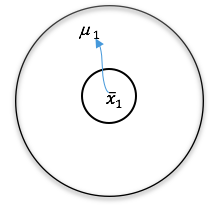
\includegraphics[width=4cm]{chapters/Chapter_11/ext_figure/x1.png} % requires the graphicx package
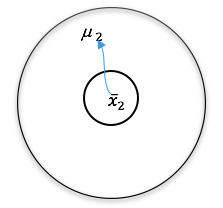
\includegraphics[width=4.3cm]{chapters/Chapter_11/ext_figure/x2.png} % requires the graphicx package
\end{figure}


As you can see, the sample circles including $\bar{x}_1$ and $\bar{x}_2$ are smaller than the entire population circles including $\mu_1$ and $\mu_2$. In other words, we do not have all the information we need to be totally sure about the exact values of  $\mu_1$ and $\mu_2$. However, as we've learned, statistics allows for sample means to estimate population means as depicted by the arrows. What's new in this chapter is that here we learn statistics can do more than just allow us to estimate values for $\mu_1$ and $\mu_2$ separately. We can also use statistics to investigate how the population means differ from one another in tandem. We do this by performing \textit{hypothesis tests} on and using confidence intervals centered around the difference between the sample means $\bar{x}_1$ and $\bar{x}_2$. Let's now turn to some formulaic examples of such tests and intervals.

Is there ``grade inflation'' in WMU?  How does the average GPA of WMU students today compare with, say 10 years ago?  Suppose a random sample of 100 student records from 10 years ago yields a sample average GPA of 2.90 with a standard deviation of 0.40.  A random sample of 100 current students today yields a sample average of 2.98 with a standard deviation of 0.45.  The difference between the two-sample means is 2.98- 2.90 = .08.  Is this proof that GPA's are higher today than 10 years ago?  Well $\dots$ first, we need to account for the fact that 2.98 and 2.90 are not the true averages but are computed from random samples.  Therefore, .08 is not the true difference, but simply an estimate of the true difference. By how much will it miss?

Note that we took differences $2.98 - $2.90 to compare average GPA.  The two averages 2.98 and 2.90 are independent, in the sense that they are based on separate and independent groups of students.  The SE of the difference is

\begin{equation}
SE_{(\bar{x}_1 - \bar{x}_2)} = \sqrt{SE_{\bar{x}_1}^2 + SE_{\bar{x}_2}^2 }
\end{equation}

whenever the two means are independent.  Equation (11.1) is similar to the equation from chapter 7, the $SE_{\hat{p}_1 - \hat{p}_2} = \sqrt{(SE_{\hat{p}_1^2} + SE_{\hat{p}_2^2 })}$, for proportions. 

Now, applying the equation from chapter 10, $SE_{\bar{X}}$ which is calculated as $\frac{s}{\sqrt{n}}$ twice, we get

\fbox{\parbox{14cm}{
Standard error of the difference between two independent means.

\begin{equation}
SE_{(\bar{x}_1 - \bar{x}_2)} = \sqrt{\frac{s_1^2}{n_1}  + \frac{s_2^2}{n_2} }
\end{equation}
}}

Continuing with the example, let $\bar{X}_1  = 2.98$ and $\bar{X}_2  = 2.90$.  Then the sample standard deviations are $S_1 = 0.45$ and $S_2 = 0.40$.   The sample sizes are $n_1 = 100$ and $n_2 = 100$.

\begin{equation*}
SE_{(\bar{x}_1 - \bar{x}_2)} = \sqrt{\frac{s_1^2}{n_1}  + \frac{s_2^2}{n_2} } = \sqrt{\frac{0.45^2}{100}  + \frac{0.40^2}{100} } = 0.06
\end{equation*}

Therefore, we can state the conclusion of the study as follows: ``The average GPA of WMU students today is .08 higher than 10 years ago, give or take .06 or so.'' We also could have used equation (11.1) instead of (11.2) in calculating the standard error:

\begin{eqnarray*}
SE_{\bar{X}_1} &=& \frac{S_1}{\sqrt{n_1}} = \frac{0.45}{\sqrt{100}} = 0.045 \\
SE_{\bar{X}_2} &=& \frac{S_2}{\sqrt{n_2}} = \frac{0.40}{\sqrt{100}} = 0.040 \\
SE_{\bar{X}_1 - \bar{X}_2} &=& \sqrt{0.045^2 + 0.040^2} = 0.06 
\end{eqnarray*}

\subsection{Using a confidence interval}

The following two sections discuss the formulas and concepts necessary for calculation and interpretation (respectively) of confidence intervals on the difference between two independent means. Let’s start with the concepts and then proceed to some formulas and examples.

\subsubsection{Confidence Interval - Concepts:}

\begin{figure}[ht]
\centering
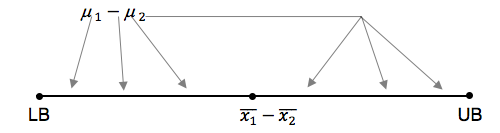
\includegraphics[width=9cm]{chapters/Chapter_11/ext_figure/2sample.png} % requires the graphicx package
\end{figure}

The interval between lower and upper bounds (LB, UB) includes some possible values of $\mu_1 - \mu_2$  (depicted by the many arrows). We need an interval around the central estimate $\bar{x}_1 - \bar{x}_2$ because of variation between samples and populations (which was depicted using concentric circles at the start of this chapter). This interval can be thought of as the ``wiggle room'' needed to estimate $\mu_1 - \mu_2$ using only $\bar{x}_1 - \bar{x}_2$.

To see how this interval can be used, it's necessary to talk about some basic properties of a difference first.  For any two numbers A and B, there are three possibilities when evaluating their difference:

\begin{enumerate}
  \item If $A - B$ is a positive number, then A is greater than B. Consider the numbers 4 and 3. If we take $4 - 3 = 1$, the answer is positive.

  \item If $A - B$ is a negative number, then B is greater than A.  For instance, if we take  $3 - 4 = -1$, the answer is negative.

  \item If $A - B$ is 0, then A = B. Consider the numbers 4 and 4: $4 - 4 = 0$.
\end{enumerate}

The same kind of reasoning holds for all the possible values of $\mu_1 - \mu_2$ between LB and UB depicted above:

\begin{enumerate}
  \item If all the values from LB to UB are positive, then 
  $\mu_1$ is significantly greater than $\mu_2$.

  \item If all the values from LB to UB are negative, then $\mu_1$ is significantly less than $\mu_2$. 

  \item If 0 is between LB and UB (inclusive), then $\mu_1$ is not significantly different from $\mu_2$.
\end{enumerate}

Note that this is just to say that the same reasoning and terminology outlined in the section on statistical significance in chapter 7 apply in the new case of a difference.  If the confidence interval for $\mu_1 - \mu_2$ does not contain 0, then 0 has been effectively excluded from the range of possible values.

\fbox{\parbox{14cm}{
When the confidence interval for $\mu_1 - \mu_2$ does not contain \textbf{zero}, we say that the difference is statistically \textbf{significant}.
}}

\subsubsection{Confidence Interval - Calculations and Examples:}

The difference of two means is a random variable with expected value and spread.  The 68\% and 95\% rules apply, i.e. the estimated difference of $\bar{x}_1 - \bar{x}_2$ should be within 1 SE of the true value 68\% of the time, and within 1.96 SE's 95\% of the time.  Following the usual reasoning,    

\begin{equation*}
(\bar{X}_1 - \bar{X}_2) \pm 1.96 SE_{(\bar{X}_1 - \bar{X}_2)}
\end{equation*}

should contain the true difference $(\mu_1 - \mu_2)$ with 95\% confidence.  Substituting (11.2), we get the following formula.

\fbox{\parbox{14cm}{
95\% confidence interval for $(\mu_1 - \mu_2)$:

\begin{equation}
  (\bar{X}_1 - \bar{X}_2) \pm 1.96 \sqrt{\frac{s_1^2}{n_1} + \frac{s_2^2}{n_2}}
\end{equation}
}}

For grade inflation, we have

\begin{equation*}
  (2.98 - 2.90) \pm 1.96 \sqrt{\frac{0.45^2}{100} + \frac{0.40^2}{100}}
\end{equation*}
\begin{equation*}
  0.08 \pm 1.96 (0.06)
\end{equation*}
\begin{equation*}
  (-0.04, 0.20)
\end{equation*}

We say that the difference in GPA averages is between $-.04$ and $.20$ with 95\% confidence.  Note that 0 has not been excluded, making simple chance variability a viable explanation for the observed difference. 

\subsection{Statistical Significance}

Let us revisit the diet study mentioned earlier.  The following table contains the mean changes in body mass index (weight in kilograms divided by height in meters squared) for the Atkins, Zone and Ornish diets. Now, compare the Atkins and Zone diets at 12 months:

\begin{table}[ht]
\centering
\caption{Mean Changes (SD) in Body Mass Index by Diet Group \& Time}
\begin{tabular}{@{} cccc @{}} \hline
Time (months) & Atkins $(n = 77)$ & Zone $(n = 79)$ & Ornish $(n = 76)$ \\ \hline
2 & -1.60(0.98) & -0.76(0.99) & -0.95(0.90) \\
6 & -2.16(2.14) & -0.73(0.90) & -0.85(1.60) \\
12 & -1.65(2.54) & -0.53(2.00) & -0.77(2.14) \\ \hline
\end{tabular}
\end{table}

On the average, Atkins lost how much more body mass index points than Zone?  The estimate of $(\mu_1 - \mu_2)$ is

\begin{equation*}
  (\bar{X}_1 - \bar{X}_2) = (-0.53) - (-1.65) = 1.12
\end{equation*}

The standard error is 

\begin{equation*}
  SE_{(\bar{X}_1 - \bar{X}_2)} = \sqrt{ \frac{(2.00)^2}{79} + \frac{(2.54)^2}{77}} = 0.367
\end{equation*}

The 95\% confidence interval for $(\mu_1 - \mu_2)$ is

\begin{equation*}
  1.12 \pm 1.96 (0.367)
\end{equation*}
\begin{equation*}
(0.84, 1.84)
\end{equation*}

Thus, even allowing for 1.96 SE's of chance variability, Atkins lost at least .40 more body mass index points than Zone (and could be as large as 1.84).   When the confidence interval for $(\mu_1 - \mu_2)$  does not contain zero, we say that the difference is statistically significant.  

\subsection{The P-value}

Continuing the example of the previous section, we might ask ``Can't the difference in averages $\bar{x}_1 - \bar{x}_2 = 1.12$ be explained by chance variability, rather than diet effect?''

The answer is ``Yes, 1.12 can occur by chance, but with very small probability.''  How small? Well, if the true difference were 0, and the SE is 0.367, then the value 1.12 is

\begin{equation*}
\frac{1.12}{0.367} = 3.05
\end{equation*}

SE's from expected value.  Using the normal curve, random variables fall as far as 3.05 or more SE's from expected value with approximately 0.0022 probability.  Since this number (also called the $P$-value) is quite small, it makes it hard to believe that the true difference is zero.  Hence, we conclude that statistically, the two means are different.  Or we can say that the means are \textit{significantly} different.

\begin{table}[ht]
\centering
\caption{Weight in pounds before and after after 12 months on diet}
\begin{tabular}{@{} crr @{}} \hline
Subject & Before & After \\ \hline
1 & 180 & 155 \\
2 & 192 & 187 \\
3 & 205 & 194 \\
4 & 166 & 176 \\
5 & 220 & 205 \\
6 & 177 & 172 \\
7 & 189 & 173 \\ \hline
Ave: & 189.9 & 180.3 \\
SD:  & 18.1 & 16.4 \\ \hline
\end{tabular}
\end{table}

\section{Paired data (before-and-after)}

In this section, we will discuss a common problem in data analysis: comparing before and after measurements.  Consider the hypothetical weight loss data in Table 11.2.

Using the notation of the previous section estimating the difference between independent means, we have

\begin{center}
\begin{minipage}[ht]{3cm}

$\bar{X}_1 = 189.9$ \\
$S_1 = 18.1$ \\
$n_1 = 7$ 
\end{minipage}
\begin{minipage}[ht]{3cm}

$\bar{X}_2 = 180.3$ \\
$S_2 = 16.4$ \\
$n_2 = 7$ 
\end{minipage}
\end{center}

What is the estimate of mean weight change after 12 months?  $\bar{x}_1 - \bar{x}_2 = 9.6$ pounds, right?  What is the standard error of this estimate? Using equation (11.2) 

\begin{equation*}
SE_{(\bar{x}_1 - \bar{x}_2)} = \sqrt{\frac{s_1^2}{n_1}  + \frac{s_2^2}{n_2} } = \sqrt{\frac{(18.1)^2}{7}  + \frac{(16.4)^2}{7} } = 9.2 \texttt{ pounds}
\end{equation*}

right?  \textbf{wrong!}

We should not use equations (11.1) or (11.2) because the two means are \textbf{not} independent, i.e. they are not calculated on independent samples.  As a matter of fact, the use of the plural `samples' is in itself wrong because we do not have two samples, we only have one! You need to watch out for this.  How many samples are there?  Before-and-after data generally consist of only one sample of subjects, each measured twice.

So how do we calculate an estimate and standard error of average weight loss?  
By calculating the amount of change from Before to After.  This amounts to taking 
differences, as shown in Table 11.3.

\begin{table}[ht]
\centering
\caption{Weight in pounds before and after after 12 months on diet}
\begin{tabular}{@{} crrr @{}} \hline
Subject & Before & After & Difference \\ \hline
1 & 180 & 155 & 25 \\
2 & 192 & 187 & 5 \\
3 & 205 & 194 & 11 \\
4 & 166 & 176 & -10 \\
5 & 220 & 205 & 15 \\
6 & 177 & 172 & 5 \\
7 & 189 & 173 & 16 \\ \hline
Ave: &  &  & 9.6 \\
SD:  &  & & 11.1 \\ \hline
\end{tabular}
\end{table}

Compare Table 11.3 to Table 11.2.  We have reduced the summary statistics to a single sample, appropriately.  The relevant statistics are now

$$ \bar{X} = 9.6,  S = 11.1,  n= 7 $$

What does the sample mean $\bar{X} = 9.6$ estimate?  It estimates the average change, right?  To be specific, it estimates the average weight loss from Month 0 to Month 12.  What is the standard error of the estimate?  Since it is just another average, the appropriate procedure is given by 

\begin{equation*}
SE_{\bar{X}} = \frac{s}{\sqrt{n}} = \frac{11.1}{\sqrt{7}} = 4.2 \texttt{ pounds}
\end{equation*}

Completing the analysis, the 95\% confidence interval for average change is

\begin{equation*}
9.6 \pm 1.96 (4.2)
\end{equation*}
\begin{equation*}
(1.4, 17.8)
\end{equation*}

Since the interval does not contain zero, the average weight change is statistically significant.

\subsection{Paired Data}

Paired data are data in which natural matchings occur.  Even when we have two samples, if each observation in one sample is uniquely matched to an observation in the other sample, then we have paired data and analysis should follow as described above.  

For example, we might want to compare the head injury of drivers versus passengers in car crashes.   In a study, automobiles were crashed into a wall at a speed of 35 MPH with dummies in the driver and front passenger seat. The head injury criterion (HIC) was measured.  Following is a selection of cars and their HIC values.

\begin{table}[ht]
\centering
\begin{tabular}{@{} lll @{}} \hline
Company & Driver & Passenger \\ \hline
Acura Integra 87        &     		599   &      597 \\
Audi 80 89              &    		600    &     515 \\
Chevrolet Camaro 91     &    		585    &     583 \\
Ford Escort 87          &     		551   &      418 \\
Honda Accord LX 91      &     	562     &    539 \\
Toyota Corolla Fx 88    &    		593     &    397 \\
Volvo 740 GLE 88        &      		519   &      445 \\ \hline
\end{tabular}
\end{table}

Since each pair of observations (e.g. 599 and 597) are uniquely matched to each other (driver and passenger HIC in the same car and crash), this is paired data and deserves paired data analysis.

\section{Key Words}


\twocolumn

\section{Exercises}

\begin{exercises}

\begin{exercise} % 1

Do credit cards with no annual fee charge higher interest rates (APR) than cards that have annual fees?  Among 29 cards surveyed, 17 had no annual fees while 12 charged an annual fee.  Among the cards with no annual fee, the average APR was 19\% (SD=8\%).  Among cards with an annual fee, the average APR was 17\% (SD=3\%).

\begin{enumerate}
  \item Estimate the difference in APR.
  \item Calculate a standard error for your estimate in (1).
  \item Calculate a 95\% confidence interval for the difference in APR between the two groups.
  \item Are interest rates significantly higher for cards with no annual fees?
  \item What is the P-value for comparing the two averages? Is the difference significant?
\end{enumerate}
\end{exercise}
\begin{solution} % 1


\end{solution}

\begin{exercise}  % 2

100 students graduating \\ with Bachelor degrees in engineering make an average of \$70,000 with a standard deviation of \$5,000 when entering the workforce. 68 students graduating with Bachelor degrees in statistics make an average of \$65,000 with a standard deviation of \$3,000 when entering the workforce. Assuming the two samples of students are independent, answer the following questions:

\begin{enumerate}
  \item What is the difference between the sample averages (engineers – statisticians)?
  \item What is the standard error of the estimate for the true difference in average entrance salaries between all engineering and statistics BA graduates?
  \item What is a 95\% confidence interval for the difference in sample averages?
  \item Do these statistics suggest that average entrance salaries for stats vs. engineering students are significantly different?
\end{enumerate}

\end{exercise}
\begin{solution}  % 2

\end{solution}

\begin{exercise}  % 3

A Junior at Southwest \\ Michigan college is debating whether to pursue an MBA after her Bachelor degree in management.  She interviews some people she \\ knows in the workforce and was able to obtain their salaries. The annual salaries (in dollars) are summarized in the following table:

\begin{tabular}{@{} lccc @{}} \hline
Degree & Aver & SD & Sample Size \\ \hline
Bachelor & \$48,286 & \$416 & 12 \\
Master   & \$59,496 & \$675 & 7 \\ \hline
\end{tabular}

\begin{enumerate}
  \item Estimate the difference in average salary between the two groups.
  \item Calculate a standard error for your estimate in (1).
  \item Calculate a 95\% confidence interval for the average difference in salary.
  \item Are MBA salaries significantly higher?
  \item What is the P-value for comparing the two averages? Is the difference significant?
\end{enumerate}
\end{exercise}  
\begin{solution}  % 3

\end{solution}

\begin{exercise}  % 4

A group of charity workers employed by a large foundation track the donations made to the foundation every month. They note that the average donations for August were somewhat higher than the average donations for September, and they want to know if this fact should worry them moving forward. Performing the correct statistical test could determine whether the average difference in donations between August and \\ September was significant. However, they \\ must first decide whether their August and  September donations are independent or not. If you were advising the charity workers, what would you tell them?
\end{exercise}
\begin{solution}  % 4


\end{solution}

\begin{exercise}  % 5

A new gasoline additive is supposed to make gas burn more cleanly and increase gas mileage in the process.  Consumer Protection Anonymous conducted a mileage test to confirm this.  They took seven of their cars, filled it with regular gas, and drove it on I-94 until it was empty.  They repeated the process using the same cars, but using the gas additive.  The recorded gas mileage follows:

\begin{tabular}{@{} llllllll @{}} \hline
Additive & 1 & 2 & 3 & 4 & 5 & 6 & 7 \\ \hline
Without & 22 & 15 & 18 & 28 & 12 & 25 & 18 \\
With    & 26 & 19 & 17 & 34 & 17 & 25 & 22 \\ \hline
\end{tabular}

\begin{enumerate}
  \item Calculate the mean difference in mileage between the two fuel types.         \item Calculate a standard error for your estimate in (1).
  \item Calculate a 95\% confidence interval for the mean mileage difference.
  \item Does the data support the claim of \\ higher gas mileage?
\end{enumerate}

\end{exercise}
\begin{solution}  % 5

\end{solution}

\begin{exercise}  % 6

The group of charity workers from the above question decide on a statistical test based on the sage wisdom you previously offered. They perform a test for significance of the average difference, and it yields a p-value of 0.50. As their stats advisor, how would you interpret this p-value with respect to whether the average difference in donations for August vs. September was significant?
\end{exercise}
\begin{solution}  % 6

\end{solution}

\end{exercises}


\onecolumn











%!Rnw root = ../../Master.Rnw

\chapter{Categorical Variables: Association or Independence}
\label{chap:ch12}

\section{Objective}

After completing this part, students should be able to:

\fbox{\parbox{14cm}{
\begin{itemize}

\item Interpret  a scatter plot.
\item Interpret the correlation coefficient $r$ \index{coefficient coefficient}  and the coefficient of determination $r^2$. \index{coefficient of determination}
\item Find and elucidate the regression line and use it to predict values of the response variable.
\item Put into words the concepts of the total, unexplained, and explained variation.  \index{unexplain variation} \index{explained variation}  \index{total variation}
\item Use correlation and regression techniques to evaluate two-variable relationships.

\end{itemize}

}}

\section{Association versus independence in an r x c table}  \index{association}

Is there an association between gender and height?  Yes, males tend to be taller than females.  A more formal way of saying this is `height distribution for males tends to be different from females.'   Is there an association between shoe size and height?  Yes,  `height distribution for men who wear size 12 is different from those who wear size 8.'    Is there an association between GPA and height?  No, `height distribution tends to be the same for 3.0 students as well as 3.5 students.'

\fbox{\parbox{14cm}{
Two variables A and B are said to be \textbf{associated} if the distribution of B tends to change with the level of the A variable.  Otherwise, they are said to be \textbf{independent} variables. 
}}

Therefore, height is associated with gender and shoe size, but independent of GPA.  

Now consider the following 3 by 4 table.  189 students entering a business school program were followed as part of an attrition (i.e. drop out, transfer) study.  The students were cross classified according to 4 categories of high school GPA $(2.0-2.5, 2.5-3.0, 3.0-3.5, 3.5-4.0)$ and 3 categories of attrition outcomes (`did not return for 2nd year,' `returned for 2nd but not for 3rd year,' `returned for 3rd year').  Is there an association between HS GPA and college attrition?

\begin{table}[ht]
\centering
\caption{Retention versus HS GPA}
\begin{tabular}{@{} lcccc @{}} \hline
& \multicolumn{4}{c}{GPA} \\
Returned & $2.0-2.5$ & $2.5-3.0$ & $3.0-3.5$ & $3.5-4.0$ \\ \hline
No --2nd yr & 25 & 3 & 4 & 6 \\
No -- 3rd yr & 14 & 7 & 4 & 6 \\
Yes -- 3rd yr & 41 & 7 & 28 & 44 \\ \hline
\end{tabular}
\end{table}

To analyze whether attrition and GPA are independent, we will analyze whether 
attrition distribution remains the same regardless of GPA level.  Let us start by looking at the 1st column (worst HS grades) and 4th column (best HS grades).  Do the distributions look the same?   The answer seems to be `no' - a bigger proportion of the 1st column never returned for their second year.  In other words, the value `25' in the very first cell is too large, implying that 'poor grades seems to be associated with first year attrition.'  If grades and attrition were independent, Table 12.1 should have looked more like Table 12.2.

\begin{table}[ht]
\centering
\caption{Expected counts (if independent)}
\begin{tabular}{@{} lcccc @{}} \hline
& \multicolumn{4}{c}{GPA} \\
Returned & $2.0-2.5$ & $2.5-3.0$ & $3.0-3.5$ & $3.5-4.0$ \\ \hline
No --2nd yr & 16 & 3 & 7 & 11 \\
No -- 3rd yr & 13 & 3 & 6 & 9 \\
Yes -- 3rd yr & 51 & 11 & 23 & 36 \\ \hline
\end{tabular}
\end{table}

This is called the table of expected counts under independence.  Observe that the row and column totals of the two tables are the same

\begin{table}[ht]
\centering
\caption{Expected counts (if independent)}
\begin{tabular}{@{} lcccccc @{}} \hline
& \multicolumn{4}{c}{GPA} \\
Returned & $2.0-2.5$ & $2.5-3.0$ & $3.0-3.5$ & $3.5-4.0$ & Total & Percent \\ \hline
No -- 2nd yr &  &  &  &  & 38 & (20.1\%) \\
No -- 3rd yr &  &  &  &  & 31 & (16.4\%)\\
Yes -- 3rd yr &  &  &  &  & 120 & (63.5\%) \\ \hline
Total        & 80 & 17 & 36 & 56 & 189 & (100\%) \\
\end{tabular}
\end{table}

Furthermore, note that 20.1\% of the data is in the first row, 16.4\% in the second row, and 65.5\% in the third row.  If we apply the same percentage breakdown to each column, we get

\begin{table}
\centering
\begin{tabular}{@{} llll @{}} \hline
$80 \times .201 = 16.08$ & $17 \times .201 = 3.42$ & $56 \times .201 = 7.24$ & $56 \times .201 = 11.26$  \\
$80 \times .164 = 13.12$ & $17 \times .164 = 2.79$ & $56 \times .164 = 5.90$ & $56 \times .164 = 9.18$  \\
$80 \times .635 = 50.80$ & $17 \times .635 = 10.80$ & $56 \times .635 = 22.86$ & $56 \times .635 = 35.56$  \\ \hline
\end{tabular}
\end{table}

Rounding off gives us the expected frequencies in Table 12.2.

\subsection{Testing for statistical association}

Statisticians will conclude `independence' if Tables 12.1 and 12.2 are close, and conclude `association' if they are far from each other.   Closeness is and farness is measured by subtraction and squaring, as follows:



\begin{equation*}
\chi^2 = \frac{(25-16.08)^2}{16.08} + \frac{(3-3.42)^2}{3.42} + \cdots + \frac{(44-35.56)^2}{35.56} = 23.42  
\end{equation*}

Note that if Tables 12.1 and 12.2 are the same, then the $\chi^2$ statistic (pronounced `chi square') in (12.1) will be 0.  If the two tables are far apart, the $\chi^2$ statistic will be large.  Statisticians use the following rule. 

\begin{center}
\fbox{\parbox{8cm}{
If the $\chi^2 > b$, then conclude statistic association
}}
\end{center}

Otherwise, conclude independence.  The number $b$ is called a critical value and depends on the dimensions of the table.  Let $r$ be the number of rows, and $c$ be the number of columns.  Let

\begin{equation*}
df = (r - 1) \times (c - 1)
\end{equation*}

be a parameter called the degrees of freedom.  Then $b$ is given by the following table.

\begin{table}[ht]
\centering
\begin{tabular}{@{} lllllllllll @{}} \hline
df & 1&2&3&4&5&6&7&8&9&10 \\
b  & 3.84&5.99&7.81&9.49&11.07&12.59&14.07&15.51&16.92&18.31 \\ \hline
\end{tabular}
\end{table}

In our example on grades and attrition, we have r=3 rows and c=4 columns, so that

\begin{equation*}
df = (3 - 1) \times (4 - 1) = 6
\end{equation*}

so the line between statistical association and independence is drawn at b=12.59.  
Since $\chi^2 = 23.42$ from (12.1), then $\chi^2 > 12.59$.   We conclude that there is significant association between high school GPA and college attrition rate.





% The correlation is a common and useful statistics.  It is a single number from $-1$ to $+1$ that indicates the strength of the relationship between the two variables.  If the number is between $-0.3$ and $+0.3 $, then we will say that the relationship is weak or non-existent. Otherwise, we will say that the relationship is either moderate or strong.  By the way, the closer we are to a $-1$ or a $+1$ the stronger the relationship.   The following example shows us how to interpret the results.
% 
% \subsection{Example 1}
% 
% Let's hypothesize that height of a male  affects the male's self-esteem.  We probably don't need to be concerned about the direction of causality; it is  unlikely that self-esteem causes a person's height.  We select a random sample of twenty males because we know that male heights are different from female heights.  By not using females heights  will simplify  the analysis.
% 
% \begin{minipage}[ht]{5cm}
% 
% {\small{
%  \begin{tabular}{@{} ccc @{}} \hline % Column formatting, @{} suppresses leading/trailing space
%      %  & \multicolumn{3}{c}{Category } \\ \hline
%      % \cmidrule(r){1-2} % Partial rule. (r) trims the line a little bit on the right; (l) & (lr) also possible
% Person & Height & Self.esteem \\ \hline
% 1 & 1.73 & 4.11 \\
% 2 & 1.81 & 4.62 \\
% 3 & 1.57 & 3.83 \\
% 4 & 1.91 & 4.44 \\
% 5	& 1.47 & 3.25 \\
% 6	& 1.52 & 3.16 \\
% 7	& 1.71 & 3.87 \\
% 8	& 1.73 & 4.18 \\
% 9	& 1.81 & 4.39 \\
% 10 & 1.75 & 3.70 \\
% 11 & 1.73 & 3.51 \\
% 12 & 1.71 & 3.22 \\
% 13 & 1.61 & 3.73 \\
% 14 & 1.57 & 3.34 \\
% 15 & 1.52 & 3.45 \\
% 16 & 1.61 & 4.06 \\
% 17 & 1.65 & 4.17 \\
% 18 & 1.71 & 3.89 \\
% 19 & 1.61 & 3.40 \\
% 20 & 1.55 &3.61 \\ \hline
% \end{tabular} }}
% 
% \end{minipage} \hfill
% \begin{minipage}[ht]{11cm}
% 
% \centering
% 
% Self Esteem by Height
% 
% <<f12_1, echo=FALSE, fig.pos="ht", fig.align="center", fig.width=3.5, fig.height=3.5, fig.path="chapters/Chapter_12/figure/">>=
%   dt12_1 <- read.csv("data/esteem.csv",header=TRUE)
%   plot( dt12_1$Self.esteem ~ dt12_1$Height.m, xlab="Height", ylab="Self Esteem")
%   lm_1 <- lm( dt12_1$Self.esteem ~ dt12_1$Height.m )
%   abline(lm_1)
% @
% 
% \end{minipage}
% 
% % \subsubsection{Scatter plot}
% 
% 
% As we review the scatter plot, we see that the direction of the relationship is positive, (i.e., as height increases, self-esteem increases).
% 
% Based on the above graphic, there appears to be a relationship between the two variables -- height and self-esteem.  But is this relationship real?  We will use the five-step model to confirm our initial assumption.
% 
% %\begin{itemize}
% %\item
% {\textbf{Step 1.}}  Making Assumptions and Meeting Test Requirements.
% 
% % Requires the booktabs if the memoir class is not being used
% \begin{table}[htbp]
%    \centering
%     \caption{Model Assumptions }
%    %\topcaption{Table captions are better up top} % requires the topcapt package
%    \begin{tabular}{@{} rl @{}} \hline % Column formatting, @{} suppresses leading/trailing space
%       % \multicolumn{2}{c}{Item} \\
%       % \cmidrule(r){1-2} % Partial rule. (r) trims the line a little bit on the right; (l) & (lr) also possible
%       1& Random sampling  \\
%       2      & Levels of Measurement are interval-ratio \\
%       3     & Bivariate normal distribution \\
%       4    & Linear relationship \\  \index{linear relationship}
%       5   & The variance of $Y$ scores is uniform for all $X$ values. \\
%       6  & Normality of residuals \\ \hline
%    \end{tabular}
%    \label{tab:t12_1}
% \end{table}
% 
% %\item
% {\textbf{Step 2.}}  State the Hypotheses. \\
%  $H_0: \rho = 0$ (there is no relationship between height and self-esteem) \\
%  $H_a: \rho \neq 0$  ($\rho$ represents the population \textbf{correlation coefficient}.)
% 
% % \item
%  {\textbf{Step 3.}}  Selecting the Sampling Distribution and Establishing the Critical Region.
% 
% 
%  % Requires the booktabs if the memoir class is not being used
% \begin{table}[htbp]
%    \centering
%    \caption{Components of correlation }
%    %\topcaption{Table captions are better up top} % requires the topcapt package
%    \begin{tabular}{@{} rcl @{}} \hline % Column formatting, @{} suppresses leading/trailing space
%       % \multicolumn{2}{c}{Item} \\
%       % \cmidrule(r){1-2} % Partial rule. (r) trims the line a little bit on the right; (l) & (lr) also possible
%       Sampling Distribution & = & t-distribution \\
%       Alpha $(\alpha)$ & = & 0.05 (two-tailed) \\
%       Degrees of Freedom  & = & $ n - 2 = 20 - 2 = 18 $  \\
%       $t_{critical}$ & = & 2.10 \\ \hline
%    \end{tabular}
%    \label{tab:t12_2}
% \end{table}
% 
% %\item
% {\textbf{Step 4.}}  Computing the Test Statistic.
% 
% The test statistic is computed by the following equation:
% 
% \begin{align*}
% t_{obtained} &= r \sqrt{ \frac{n - 2}{1 - r^2}} \\
%               &= 0.721 \sqrt{ \frac{20 - 2}{1 - 0.721^2}} \\
%               &= 4.4145 \\
% \end{align*}
% 
% From figure \ref{fig:f12_2} on page \pageref{fig:f12_2} (MINITAB printout), we find Pearson Correlation coefficient, $r = 0.721$.  In step 4, we see the test statistic ($t_{obtained}$) is equal to 4.41.
% 
%   \begin{figure}[ht]
%     \centering
%     \caption{MINITAB Correlation Analysis}
%     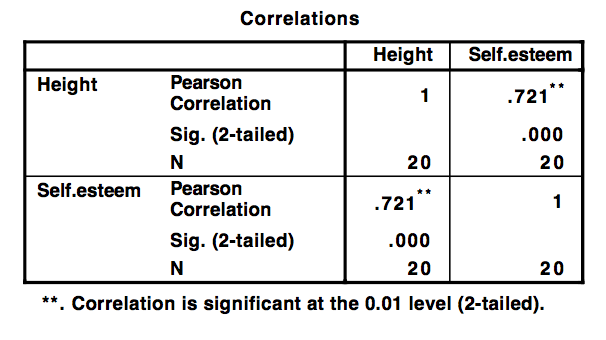
\includegraphics[width=10cm]{chapters/Chapter_12/ext_figure/zCorrA.png} % requires the graphicx package
%     \label{fig:f12_2}
%  \end{figure}
% 
% %\item
% {\textbf{Step 5:}} Deciding and Interpreting the Results of the Test
% 
% Since the $t_{obtained}$ (test statistic) is greater than the $t_{critical}$ value ($ 4.41 > 2.10 $), we reject the null hypothesis.  Thus, we can say that there is a strong, positive relationship  between male height and male self-esteem.
% %\end{itemize}
% 
% % \pagebreak
% \section{What is Linear Regression?}  \index{linear regression}
% 
% Regression analysis is a method that we use when the explanatory and response variables are both numeric, i.e., interval-ratio variables, for example, weights, heights, volumes, and temperature.  The easiest way of knowing if the regression is the appropriate method is to see a scatter plot of the data.  The researcher will choose the linear regression model if there is an apparent (linear) relationship.  Let's examine an example that will help explain the process.
% 
% Let's consider the relationship between the percent change of city population growth  from 2000 and 2008 and the number of annual car thefts.  As a researcher, we review the level of measurement and find that both variables are interval-ratio.  So we consider using the scatter plot.  It has two dimensions, the x-axis which is the explanatory (X) variable and the y-axis which is the response (Y) variable that we want to predict.
% 
% \begin{minipage}[ht]{5cm}
% 
% \centering
% {\small{
%    \begin{tabular}{@{} cc @{}} \hline % Column formatting, @{} suppresses leading/trailing space
%      %  & \multicolumn{3}{c}{Category } \\ \hline
%      % \cmidrule(r){1-2} % Partial rule. (r) trims the line a little bit on the right; (l) & (lr) also possible
%      Growth & Car.theft \\ \hline
%      9.8 & 118 \\
%      5.7 & 204 \\
%      1.3 & 294 \\
%      2.7 & 163 \\
%      26.8 & 764 \\
%      3.4 & 95 \\
%      16.8 & 392 \\
%      11.2 & 581 \\
%      8.6 & 601 \\
%      2.8 & 144 \\ \hline
%    \end{tabular}
% }}
% 
%   \end{minipage} \hfill
% \begin{minipage}[ht]{10cm}
% 
% \centering
% 
% Figure: 12.3, Car Theft by Growth
% 
% <<label=f12_3, echo=FALSE, fig.pos="ht", fig.align="center", fig.width=3.6, fig.height=3.6, fig.path="chapters/Chapter_12/figure/">>=
%   dt12_2 <- read.csv("data/EX12A.csv",header=TRUE)
%   plot( dt12_2$Car.theft ~ dt12_2$Growth, xlab="Growth", ylab="Car Theft")
%   lm_2 <- lm( dt12_2$Car.theft ~ dt12_2$Growth )
%   abline( lm_2 )
%   b_1 <- lm_2$coefficient[2]
%   b_0 <- lm_2$coefficient[1]
% 
%   xx_11 <- 20
%   xy_11 <- 0
% 
%   xy_22 <- b_0 + b_1 * 20
%   lines(c(xx_11,xy_11), c(xy_22, xy_22), col="red")
%   lines(c(xx_11, xx_11), c(xy_11, xy_22), col="red")
% @
% 
% \end{minipage}
% 
% \subsubsection{Interpreting Scatter Plot}
% 
% The pattern of points on the graph seems to indicate that  city growth (percent change from 2000 to 2008)  increases so does the number of auto thefts increase.  To demonstrate this pattern, we can draw a straight line that approximates the best fit for the points (See Figure 12.3).
% 
% \subsubsection{Does a Relationship Exist?}
% 
% The definition of an association states that the relationship between two variables will vary in the same direction either positive or negative.  As the \emph{X}-variable increases, the \emph{Y}-variable will increase (decrease if the direction is negative).  If a linear relationship exists between these two variables, then the best-fitted line through the points will not be parallel with the x-axis.
% % In other words, the \emph{X-Y} pair represents a point on the scatter plot.
% In a subsequent section, we will use a statistical method to test this hypothesis.
% 
% \subsubsection{How Strong is the association?}
% 
% The density around the fitted regression line assesses the strength of this relationship.  If the relationship is perfect, then the points of \emph{X - Y} will lie  on the fitted regression line.  Otherwise, the relationship becomes weaker when the data points are away from the fitted regression line.  What we are talking about here is the correlation coefficient.
% 
% From Figure \ref{fig:f12_4} on page \pageref{fig:f12_4} (MINITAB printout), we find Pearson Correlation coefficient, $r = 0.773$ indicating that we have a high correlation between city growth and car theft.  Note the arrow is pointing to the correlation coefficient.
% 
%   \begin{figure}[ht]
%     \centering
%     \caption{MINITAB Correlation Analysis}
%     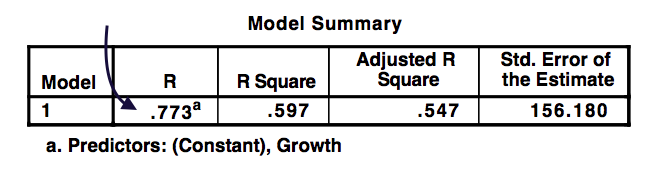
\includegraphics[width=11cm]{chapters/Chapter_12/ext_figure/zEX12corr.png} % requires the graphicx package
%     \label{fig:f12_4}
%  \end{figure}
% 
% \subsubsection{Predicting response variable using the scatter plot}
% 
% We can use the scatter plot for prediction.  To show this procedure, let's look at the relationship between city growth and annual car thefts illustrated in Figure 12.3.  Let's say that we want to predict the number of car thefts in a city that has grown by 20 percent from 2000 to 2008.  The predicted score on \emph{Y} (indicated by $\hat{Y}$) to discriminate between the predictions of \emph{Y} from the actual \emph{Y} scores.  First, we should locate 20 on the x-axis and then draw a straight line parallel with the y-axis and to the regression line.  From the regression line, draw another line that is parallel to the x-axis to the y-axis.  The predicted \emph{Y} ($\hat{Y}$) is found at the point where the line crosses the y-axis.  We predict that cities that have grown by 20 percent from 2000 to 2008, the number of car thefts would be around 600 per year.  Later, we will develop a model for making this prediction.
% 
% \subsubsection{The Regression Line}
% 
% Using the above method is crude because trying to fit a line through a cloud of points by using a free hand.  A mathematical method has been developed and implemented in many statistical programs, such as SPSS, MINITAB, SAS, R, etc., to solve this fundamental equation:
% 
% \begin{equation}
% Y = a + bX
% \end{equation}
% 
% \begin{align*}
% Y &= Dependent \hspace{1mm} Variable \\
% a &= Y \hspace{1mm} intercept \\  \index{intercept}
% b &= Slope \\  \index{slope}
% X &= Independent \hspace{1mm} Variable
% \end{align*}
% 
% \subsubsection{Determining the y-intercept (a)}
% 
% From the MINITAB output Figure \ref{fig:f12_5}, let's determine the y-intercept of this  problem.
% 
%   \begin{figure}[ht]
%     \centering
%     \caption{MINITAB Regression Analysis}
%     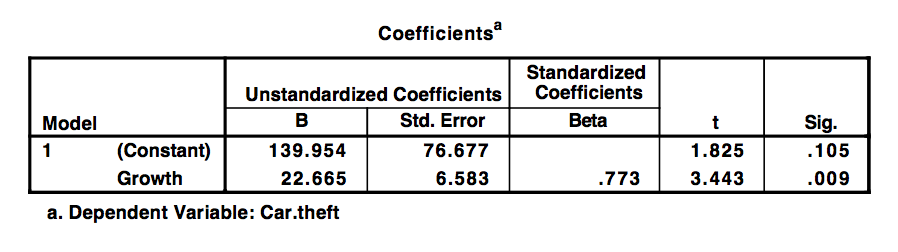
\includegraphics[width=11cm]{chapters/Chapter_12/ext_figure/zRegD.png} % requires the graphicx package
%     \label{fig:f12_5}
%  \end{figure}
% 
%  After reviewing Figure \ref{fig:f12_5}, we find column B and row (Constant) (a) is 139.954.  Our interpretation of the y-intercept is 139.954 when \emph{X} = 0.  Now keep this number in mind as we determine the slope because we will use these two numbers to predict the annual car theft based on the percent change that a city experienced from 2000 to 2008.
% 
% \subsubsection{Determine the slope (b) }
% 
% From the MINITAB output Figure \ref{fig:f12_5}, let's identify the slope of this  problem.
% 
% After reviewing Figure \ref{fig:f12_5}, we find column B and row Growth that the slope (b) is 22.665.  Our interpretation of the slope is that as the percentage change of the cities growth increases by 1 percent, the number of car thefts increases by 22.665 per year.  Let's evaluate the slope with the five step model.
% 
% \begin{itemize}
% \item {\textbf{Step 1.}}  Making Assumptions and Meeting Test Requirements.
% 
% % Requires the booktabs if the memoir class is not being used
% \begin{table}[htbp]
%    \centering
%     \caption{Model Assumptions}
%    %\topcaption{Table captions are better up top} % requires the topcapt package
%    \begin{tabular}{@{} rl @{}} \hline % Column formatting, @{} suppresses leading/trailing space
%       % \multicolumn{2}{c}{Item} \\
%       % \cmidrule(r){1-2} % Partial rule. (r) trims the line a little bit on the right; (l) & (lr) also possible
%       1 & Random sampling  \\
%       2       & Levels of Measurement are interval-ratio \\
%       3       & Bivariate normal distribution \\
%       4       & Linear relationship \\
%       5       & Variance of $Y$ scores is uniform for all $X$ values. \\
%       6       & Normality of residuals. \\ \hline
%    \end{tabular}
%    \label{tab:t12_3}
% \end{table}
% 
% \item {\textbf{Step 2.}}  State the Hypotheses. \\
%  $H_0: \beta = 0$ (there is no relationship between percent change of a city and car theft) \\
%  $H_a: \beta \neq 0$ (where $\beta$ represents the population \textbf{slope}.)
%  \item {\textbf{Step 3.}}  Selecting the Sampling Distribution and Establishing the Critical Region.
% 
% 
%  % Requires the booktabs if the memoir class is not being used
% \begin{table}[htbp]
%    \centering
%     \caption{Components of correlation}
%    %\topcaption{Table captions are better up top} % requires the topcapt package
%    \begin{tabular}{@{} rcl @{}} \hline % Column formatting, @{} suppresses leading/trailing space
%       % \multicolumn{2}{c}{Item} \\
%       % \cmidrule(r){1-2} % Partial rule. (r) trims the line a little bit on the right; (l) & (lr) also possible
%       Sampling Distribution & = & t-distribution \\
%       Alpha $(\alpha)$ & = & 0.05 (two-tailed) \\
%       Degrees of Freedom  & = & $ n - 2 = 10 - 2 = 8 $  \\
%       $t_{critical}$ & = & 2.3060 \\ \hline
%    \end{tabular}
%    \label{tab:t12_4}
% \end{table}
% 
% \item {\textbf{Step 4.}}  Determine the Test Statistic.
% 
% The test statistic is determined from  the following table.
% 
% From Figure \ref{fig:f12_6}, (MINITAB printout), we find the slope (b) = 22.665.  The test statistic $t$ is 3.443, from row Growth and column $t$.
% 
%   \begin{figure}[ht]
%     \centering
%     \caption{MINITAB Regression Analysis}
%     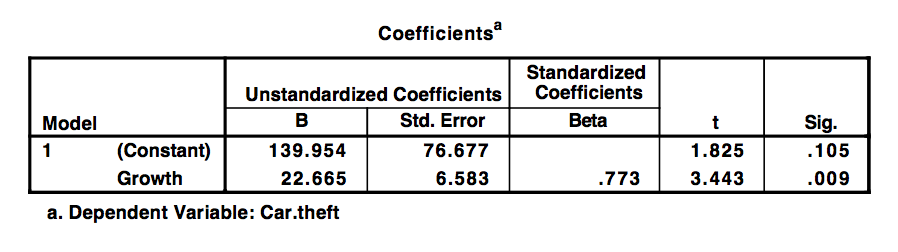
\includegraphics[width=11cm]{chapters/Chapter_12/ext_figure/zRegD.png} % requires the graphicx package
%     \label{fig:f12_6}
%  \end{figure}
% 
% \item {\textbf{Step 5:}} Making a Decision and Interpreting the Results of the Test
% 
% Since the $t_{obtained}$ (test statistic) is greater than the $t_{critical}$ value ($ 3.443 > 2.2060 $), we reject the null hypothesis. Thus we can interpret the slope by saying as the percent change in  city increases by one, the number of annual car thefts increases by 22.7.
% 
% \end{itemize}
% 
% \subsubsection{Prediction}
% 
% Now let's put it all together.  We have an equation.  We will use the same \emph{X}-value = 20 that we used when we used a graphical solution for this problem.
% 
% \begin{align*}
% \hat{Y} &= a + b(X) \\
% CarThefts &= 139.954 + 22.665(Growth) \\
%           &= 139.954 + 22.665(20) \\
%           &= 593.3
% \end{align*}
% 
% We can now say that a city that had percent change growth of 20 percent will have an estimated 593 automobiles stolen in one year.
% 
% \subsubsection{Interpreting the Regression}
% 
% What variables can she collect to predict the final exam score of an Introductory Statistics course?  Statistics instructors have been asking this question for a long time.  An instructor gathered,  (four explanatory variables (MT1, MT2, Proj, HW)), data from 64 of her statistics class students and did the following analysis.
% 
% \subsubsection{Descriptive Statistics}
% 
% Table \ref{tab:t12_5} reports the basic descriptive statistics for the variables.  The average final exam score is 156.1 with a score ranging  from 75 to 191.  The mean mid-term  test one score is 86.1 with a score ranging from 50 to 99.  As consultants, we should ask ourselves, what explanatory variables should we use to predict the final exam score.
% 
%  % Requires the booktabs if the memoir class is not being used
% \begin{table}[htbp]
%    \centering
%     \caption{Descriptive Statistics }
%    %\topcaption{Table captions are better up top} % requires the topcapt package
%    \begin{tabular}{@{} lccccc @{}} \hline % Column formatting, @{} suppresses leading/trailing space
%        &  \multicolumn{5}{c}{Descriptive Statistics} \\
%       % \cmidrule(r){1-2} % Partial rule. (r) trims the line a little bit on the right; (l) & (lr) also possible
%       Statistics & Final & MT1 & MT2 & Proj & HW \\ \hline
%       Mean & 156.1 & 86.1 & 74.2 & 10.1 & 72.3 \\
%       Standard deviation & 24.47 & 11.51 & 18.59 & 1.16 & 11.69 \\
%       N & 64 & 64 & 64 & 64 & 64 \\ \hline
%    \end{tabular}
%    \label{tab:t12_5}
% \end{table}
% 
% \begin{itemize}
% \item Where
%   \begin{itemize}
%   \samepage
%   \item Final --  Exam score
%   \samepage
%   \item MT1 -- Midterm exam one score
%   \samepage
%   \item MT2 -- Midterm exam two score
%   \samepage
%   \item Proj -- Project score
%   \samepage
%   \item HW -- Homework score
%   \samepage
%   \end{itemize}
% \end{itemize}
% 
% 
% \subsubsection{Correlation matrix}
% 
%  % Requires the booktabs if the memoir class is not being used
% \begin{table}[htbp]
%    \centering
%     \caption{Pearson Correlation Coefficient}
%    \begin{tabular}{@{} lccccc @{}} \hline % Column formatting, @{} suppresses leading/trailing space
%       % &  \multicolumn{5}{c}{Pearson Correlation} \\
%       % \cmidrule(r){1-2} % Partial rule. (r) trims the line a little bit on the right; (l) & (lr) also possible
%       Statistics & Final & MT1 & MT2 & Project & HW \\ \hline
%       Final & 1  \\
%       MT1   & \fbox{0.751} & 1 \\
%       MT2   & 0.543 & 0.454 & 1 \\
%       Proj & 0.087 & 0.101 & -0.032 & 1 \\
%       HW      & 0.273 & 0.301 & 0.218 & 0.093 & 1 \\ \hline
%    \end{tabular}
%    \label{tab:t12_6}
% \end{table}
% 
% After reviewing the correlation matrix (Table \ref{tab:t12_6}), we see that at the intersection of Final and MT1 has a correlation coefficient ($r = 0.751$) which is the largest number in the matrix.  This number tells us that we have a strong positive relationship between the mean final exam score and the mean mid-term exam one score.  The coefficient of determination ($r^2 = 0.564$) which tells us that the mid-term one score explains 56.4 percent of the variance in the final exam score.
% 
% \subsubsection{Scatter plot}  \index{scatter plot}
% 
% The next step in assessing an association between two interval-ratio variables is the scatter plot.  Figure \ref{fig:f12_7} displays the final exam scores on the vertical, \emph{Y}, axis, and the mid-term evaluation one score on the horizontal, \emph{X}, axis.
% 
% <<label=f12_7, echo=FALSE, fig.pos="ht", fig.align="center", fig.width=8, fig.height=8, fig.cap="Mid-term 1 Exam", out.width="6cm", fig.path="chapters/Chapter_12/figure/">>=
%   dt12_3 <- read.csv("data/grades.csv",header=TRUE)
%   plot( dt12_3$Final ~ dt12_3$MT1, xlab="Mid-Term 1 ", ylab="Final")
%   lm_3 <- lm( dt12_3$Final ~ dt12_3$MT1 )
%   abline( lm_3 )
%   b_1 <- lm_3$coefficient[2]
%   b_0 <- lm_3$coefficient[1]
% @
% 
% What can we say about the relationship?  The regression line is \emph{not} horizontal, so there is an association between these two variables.  The graph shows points scattered around the regression line, and we can see that we have a strong positive relationship.
% 
% \subsubsection{Regression Equation}  \index{regression equation}
% 
% The next step is to determine the regression equation.
% 
%   \begin{figure}[ht]
%     \centering
%     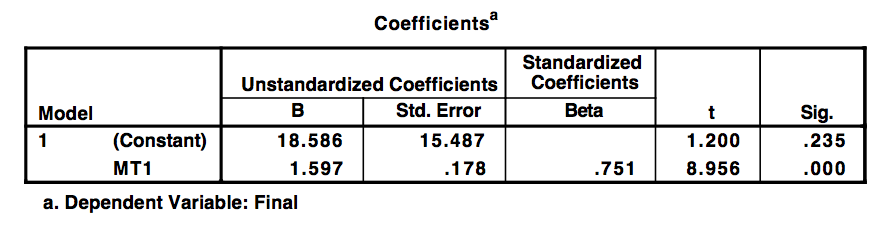
\includegraphics[width=12cm]{chapters/Chapter_12/ext_figure/zRegE.png} % requires the graphicx package
%     \caption{MINITAB Regression Analysis }
%     \label{fig:f12_8}
%  \end{figure}
% 
% After reviewing Figure \ref{fig:f12_8}, we find the \emph{Y}-intercept (\emph{a}) is 18.586, row (constant) and column B.  The slope (\emph{b}) is 1.597, row MT1 and column B.
% 
% \begin{align*}
%     Y &= a + bX \\
% Final &= 18.586 + 1.597(MT1)
% \end{align*}
% 
% The interpretation of the slope is as mid-term one exam scores increase by one unit, the final exam score increase by 1.597 points.
% 
% \subsubsection{Diagnostics}
% 
% \begin{itemize}
% \item Coefficient of determination:  \index{coefficient determination}
%   \begin{itemize}
%   \item $r^2 = \frac{explained Variation}{total Variation}$
%   \item We measure the explained variation from the average of the \emph{Y}-variable to the predicted \emph{Y}-variable.
%   \item We compute the unexplained variation from the observed \emph{Y}-variable to the predicted \emph{Y}-variable.
%   \item We determine the total change from the observed \emph{Y}-variable to the average of the \emph{Y}-variable.
%   \end{itemize}
% 
% \item There is one other thing that we should look at --  residuals.
%   \begin{itemize}
%   \item For each data point, we should compute the difference:
% 
%   \begin{equation}
%   Residual_i =  observedValue_i - predictedValue_i
%   \end{equation}
% 
% 
%   \item The histogram of the residuals should be  bell-shaped as in Figure \ref{fig:f12_9}.
% 
% 
% %\begin{minipage}[ht]{6.5cm}
% 
%   <<label=f12_9,  echo=FALSE, fig.pos="ht", fig.align="center", fig.width=8, fig.height=8, fig.cap="Histogram of Residuals", out.width="6cm", fig.path="chapters/Chapter_12/figure/">>=
%   hist(lm_3$residuals)
%   @
% 
% %\end{minipage} \hfill
% %\begin{minipage}[ht]{6.5cm}
% 
%   <<label=f12_10, echo=FALSE, fig.pos="ht", fig.align="center", fig.width=8, fig.height=8, fig.cap="Residual Plot", out.width="6cm", fig.path="chapters/Chapter_12/figure/">>=
% 
%   plot( lm_3$residuals ~ lm_3$fitted.values, xlab="Final -- fitted values ", ylab="Residuals")
%   abline( 0,0 )
% @
% 
% %\end{minipage}
% 
%   \item Let's look at Figure \ref{fig:f12_9}.  Here we can draw a nearly normal-shaped curve over the histogram.
%   \end{itemize}
% 
% \item Another assumption that we need to consider is homoscedasticity, i.e.,  \index{homoscedasticity} is the variance of \emph{Y} scores uniform across all values of \emph{X}.
% 
%   \begin{itemize}
% 
%   \item Figure \ref{fig:f12_10} shows a pattern of points that is uniform.
% 
%   \end{itemize}
% 
% \end{itemize}
% 
% \subsubsection{Summary}
% 
% To conclude this analysis, the linear regression equation, the correlation coefficient, and coefficient of determination suggest that there exist a positive and strong relationship between the first mid-term exam score  and the final exam score.  The amount of unexplained variation (total variation - explained variation, i.e., 100 - 55 = 45) suggests that there may be other variables besides first mid-term exam that have a significant influence on the final exam score.
% 
% We should note one limitation of the simple linear regression.  First correlation is not the same as causation.  In other words, two variables that are highly correlated does not necessarily suggest that there is a causal relationship.  We could take these results to support the proposition that higher mid-term exam scores lead to higher final exam scores, the mere existence of a relationship -- even a strong connection in the direction predicted by the theory -- does not prove that one variable causes the other.
% 
% \section{Key Words}
% 
% \colorbox{lgray}{\parbox{15cm}{
% \begin{minipage}[ht]{6cm}
% \begin{itemize}
% \item Bivariate normal distribution
% \item Coefficient of discrimination
% \item Correlation matrix
% \item Explained variation
% \item Homoscedasticity
% \item Linear relationship
% \item Pearson's r
% \end{itemize}
% 
% \end{minipage} \hfill
% \begin{minipage}[ht]{6cm}
% \begin{itemize}
% \item Regression line
% \item Scatter plot
% \item Slope
% \item Total variation
% \item Unexplained variation
% \item \emph{Y}-intercept
% \item $\hat{Y}$
% \end{itemize}
% \end{minipage}
% }}

\twocolumn
\section{Exercises}
 
\begin{exercises}

\begin{exercise} % 1

In a study of drug usage by students at a large university, data was obtained regarding hard liquor experience of smokers and nonsmokers.

\begin{tabular}{@{} lll @{}} \hline
Hard-Liquor Use & Nonsmokers & Smokers \\ \hline
Once or more & 15 & 23 \\
Never        & 56 & 18 \\ \hline
\end{tabular}

Is liquor use associated with smoking?  Conduct a chi-square test to assess significance of association.

\end{exercise}
\begin{solution} % 1

\end{solution}

\begin{exercise} % 2

2.	During the filming of an original comedy special, Netflix monitored whether audience members who received free tickets laughed during the show (LDS). The results follow:

\begin{table}[ht]
\centering
\begin{tabular}{@{} llll @{}} \hline
& \multicolumn{2}{c}{LDS} \\
Free Tickets & Yes & No & Total \\ \hline
Yes & 17 & 1  & 18 \\
No  & 28 & 43 & 71  \\ \hline
Total & 45 & 44 & 89 \\ \hline
\end{tabular}
% \caption{LDS -- Laughed During Show}
\end{table}

\begin{enumerate}
  \item Calculate the expected count for audience members who did not receive a free ticket and did not laugh during the \\ show.
  \item Calculate the expected count for audience members who did not receive a free ticket and did laugh during the show.
  \item Calculate the expected count for audience members who did receive a free \\ ticket and did laugh during the show.
  \item Calculate the expected count for audience members who did receive a free \\ ticket and did not laugh during the \\ show.
  \item Calculate the chi-square test statistic.
  \item What do you conclude?
\end{enumerate}

\end{exercise}
\begin{solution}  % 2

\end{solution}

\begin{exercise} % 3

A study investigating the association between size of cars and country found the following frequency counts:

\begin{table}[ht]
\centering 
\begin{tabular}{@{} lrrrr @{}} \hline
         & US & Japan & UK & France \\ \hline
Economy & 21 & 24 & 33 & 55 \\
Compact & 27 & 35 & 37 & 40 \\
Full size & 36 & 11 & 12 & 4 \\
Luxury  & 15 & 3 & 7 & 8 \\ \hline
\end{tabular}
\end{table}

Is there evidence of a significant relationship between size of car and country, or are the two variables independent?
\end{exercise}
\begin{solution} % 3

\end{solution}

\begin{exercise} % 4

Suppose Netflix held another special, collected data, and had a statistician calculate and interpret the chi square test statistic. However, this time, the statistician found insignificant differences between observed and expected counts for all those who did and did not laugh with and without free tickets. What is the appropriate conclusion in this case?
\end{exercise}
\begin{solution} % 4

\end{solution}

\begin{exercise} % 5

Computer-controlled cameras are being used to ticket automobile \\ drivers for speeding and running red lights.  These devices are operated by private firms and have an incentive to pull in as many \\ drivers as they can.  Although approximately 70\% of the motorists stoically accept and pay these tickets, others resent this procedure and fight the ticket.  A frequency table with \\ marginal totals is given below. 

\begin{table}[ht]
\centering
\begin{tabular}{@{} llll @{}} \hline
& \multicolumn{2}{c}{Volation} \\
Ticket & Run Red Light & Speeding & Total \\ \hline
Pay  &  &   & 140 \\
Fight   &  &  & 60  \\ \hline
Total & 60 & 140 & 200 \\ \hline
\end{tabular}
% \caption{LDS -- Laughed During Show}
\end{table}

\begin{enumerate}
  \item Compute the table of expected frequencies.
  \item Suppose we know that 1/3 of those who were ticketed for running a red light \\ fought the ticket.  Is this enough information to conduct a test of association or independence between the two variables?
  \item Using the information in (b), compute the chi-square statistic for testing independence or association between the two variables.
  \item What is the correct degrees of freedom to use?
  \item What is the conclusion of your test?
\end{enumerate}

\end{exercise}
\begin{solution} % 5

\end{solution}
\end{exercises}

\onecolumn


%!Rnw root = ../../Master.Rnw

\chapter{Correlation}
\label{chap:ch13}

\section{Objective}

After completing this part, students should be able to:

\fbox{\parbox{14cm}{
\begin{itemize}

\item Interpret  a scatter plot.
\item Interpret the correlation coefficient $r$ \index{coefficient coefficient}  and the coefficient of determination $r^2$. \index{coefficient of determination}
\item Find and elucidate the regression line and use it to predict values of the response variable.
\item Put into words the concepts of the total, unexplained, and explained variation.  \index{unexplain variation} \index{explained variation}  \index{total variation}
\item Use correlation and regression techniques to evaluate two-variable relationships.
\end{itemize}

}}

The following data appeared in the Wall Street Journal in 1984.  Advertisements were selected by an annual survey conducted by Video Board Tests, Inc., a New York ad-testing company, based on interviews with 20,000 adults who were asked to name the most outstanding TV commercial they had seen, noticed, and liked. The retained impressions were based on a survey of 4,000 adults, in which regular product users were asked to cite a commercial they had seen for that product category in the past week.  `TV Ad Budget' was the 1983 advertising budget in \$ millions.  `Impressions' is the estimated number of million impressions per week.

\begin{table}[ht]
\centering 
\begin{tabular}{@{} lrr @{}} \hline
& \multicolumn{1}{c}{TV Ad} \\
Company & Budget & Impressions \\ \hline
Miller Lite & 50.1 & 32.1 \\
Pepsi & 74.1 & 99.6 \\
Stroh's & 19.3 & 11.7 \\
Fed'd Express & 22.9 & 21.9 \\
Burger King & 82.4 & 60.8 \\
Cola-Cola & 40.1 & 78.6 \\
McDonald's & 185.9 & 92.4 \\
MCI & 26.9 & 50.7 \\
Diet Cola & 20.4 & 21.4 \\
Ford & 166.2 & 40.1 \\
Levi's & 27.0 & 40.8 \\
Bud Lite & 45.6 & 10.4 \\
ATT/Bell & 154.9 & 88.9 \\
Calvin Klein & 5.0 & 12.0 \\
Wendy's & 49.7 & 29.2 \\
Polandoid & 26.9 & 38.0 \\
Shasta & 5.7 & 10.0 \\
Meow Mix & 7.6 & 12.3 \\
Oscar Meyer & 9.2 & 23.4 \\
Crest & 32.4 & 71.1 \\
Kibbles 'n Bits & 6.1 & 4.4 \\ \hline
\end{tabular}
\end{table}

Figure 13.1 shows a scatterplot of Impressions Score (Y) versus Ad Spending (X). Note that the points seem to loosely fall around a line sloped upwards.  We say that there is a positive linear association, or a linear relationship between spending and the number of impressions made.  

If the points fall around a straight line sloped downwards, we say that there is a negative association.

\begin{figure}[ht]
\centering



{\centering 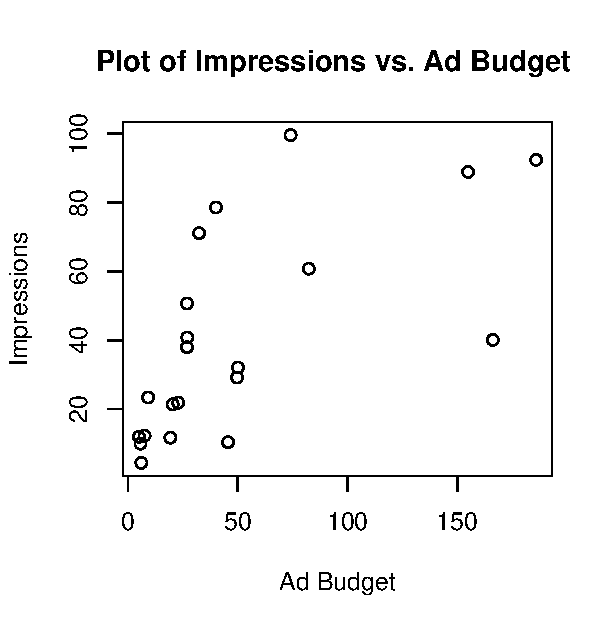
\includegraphics[width=8cm]{figure/LBL13a-1} 

}



\end{figure}

The direction and strength of association is often expressed in a single number called the (Pearson) \textit{correlation coefficient}.  Typically denoted by $r$, the correlation coefficient $r$ is a number between $-1$ and $+1$, inclusive.  A value of $r = 0$ means that no linear association exists; the points either look like a random scatter or fall around a horizontal line.  A value of $r = +1$ indicates a perfectly linear relationship; all the points fall on a straight line sloped upwards.  If $r = -1$, all the points fall on a straight line sloped downwards. The correlation between TV Ad Budget and Impressions in the data above is $+0.65$.

Figure 13.2 on the following page shows various scatterplots with different correlations.  Although $0.5$ is halfway between $0$ and $1$, note that the plot corresponding to $r = 0.5$ barely shows a pattern of association.  In practice, plots can show correlations up to $0.3$ purely by accident (e.g., correlation between GPA and, say, shoe size).  When correlation reaches $+1$ or $-1$, all points fall on a straight line.

\begin{figure}[ht]



\caption{Correlation plots (from top to bottom, r = -0.6210, 0.4256, -0.9787, 0.9967)}


{\centering 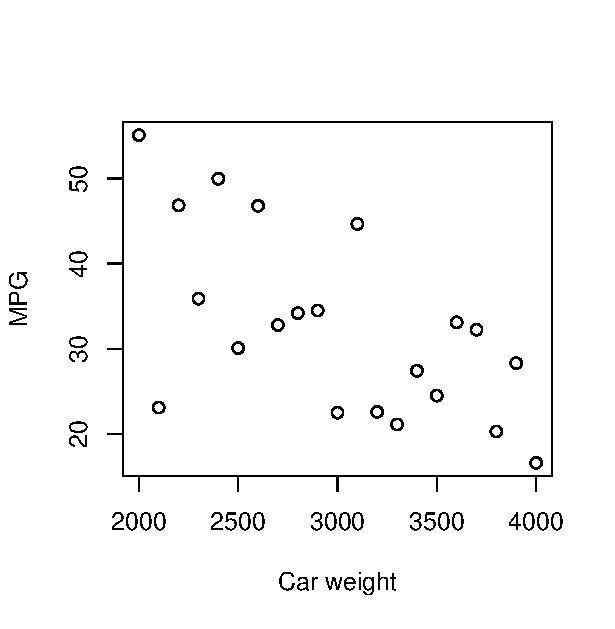
\includegraphics[width=4cm]{figure/LBL13b-1} 

}





{\centering 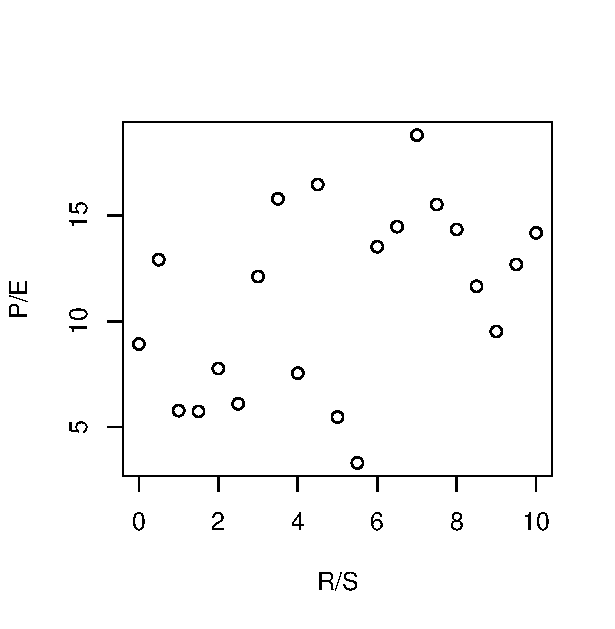
\includegraphics[width=4cm]{figure/LBL13c-1} 

}





{\centering 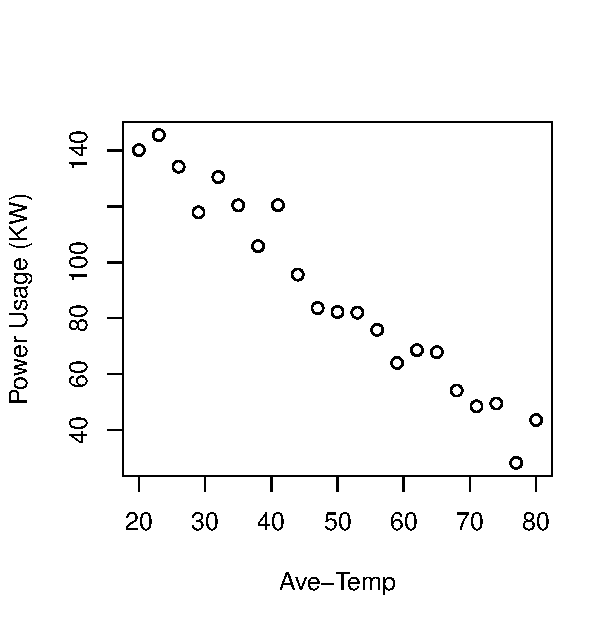
\includegraphics[width=4cm]{figure/LBL13d-1} 

}





{\centering 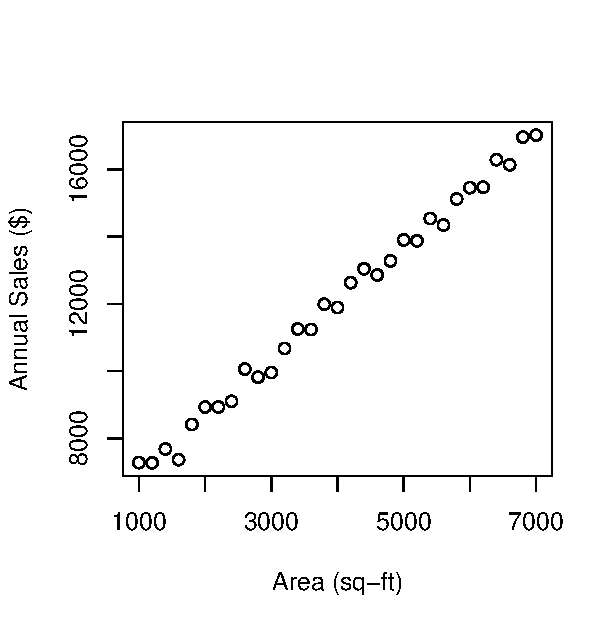
\includegraphics[width=4cm]{figure/LBL13e-1} 

}



\end{figure}

\section{Computing the Pearson Correlation Coefficient}

The following numerical example shows how to calculate $r$.  We will break the calculations down into four steps.

\begin{enumerate}
\item Calculate the mean and SD of X and Y.

\begin{table}[ht]
\centering
\begin{tabular}{@{} ccc @{}} \hline
Sample & X & Y \\ \hline
1 & 1 & 3 \\
2 & 3 & 9 \\
3 & 4 & 7 \\
4 & 4 & 9 \\
5 & 5 & 15 \\
6 & 7 & 11 \\ \hline
Average & 4 & 9 \\
SD  & 2 & 4 \\ \hline
\end{tabular}
\end{table}

\item Calculate the Z-scores from equation (4.1) on page 42.  

$$ Z_x = \frac{X - \bar{X}}{S_x} = \frac{X - 4}{2} \texttt{ and } Z_y = \frac{Y - \bar{Y}}{S_y} = \frac{Y - 9}{4} $$

\item Multiply the Z-scores and add up.

\begin{table}[ht]
\centering
\begin{tabular}{@{} ccc @{}} \hline
$Z_x$ & $Z_y$ & $Z_x Z_y$ \\ \hline
-1.5 & -1.5 & 2.25 \\
-0.5 & 0 & 0 \\
0 & -0.5 & 0 \\
0 & 0 & 0 \\
0.5 & 1.5 & 0.75 \\
1.5 & 0.5 & 0.75 \\ \hline
Average &  & 3.75 \\
\end{tabular}
\end{table}

\item Finally, the correlation is the sum divided by ($n - 1$).

$$ r = \frac{3.75}{6 - 1} = 0.75 $$
\end{enumerate}

The whole process can be summarized in the following formula.

\begin{center}
\fbox{\parbox{10cm}{
\textbf{The Correlation coefficient r:} 

\begin{equation}
r = \frac{ \sum Z_x Z_y }{n - 1} 
\end{equation}
}}
\end{center}

Consider the Ad Spending example at the start of this chapter.  Many of the (X, Y) points are simultaneously above average, since companies that have higher than average Advertising Spending also have higher than average Impressions.  

Both $X - \bar{X}$  and $Y - \bar{Y}$ are positive for these companies, therefore $Z_x$  and $Z_y$  are both positive, and the product ($Z_x$)($Z_y$)  is positive for these companies.  Most of the remaining companies have lower than average Spending and lower than average Impressions.  Both $Z_x$  and $Z_y$  are negative for these companies, but the product ($Z_x$)($Z_y$) is still positive!  Hence the numerator in (13.1) tends to be a large positive number for the Ad Spending data.

If the points were sloped downwards, then high X-values tend to go with low Y-values, and many points have negative product ($Z_x$)($Z_y$).  This is how the correlation formula (13.1) works.  

\fbox{\parbox{14cm}{
If $X$ and $Y$ tend to be simultaneously above average or simultaneously below average, then the correlation coefficient will be \textbf{positive}.  

If above-average X values tend to be paired with below-average Y values, then the correlation coefficient will be \textbf{negative}. 

}}

\twocolumn

\section{Exercises}

\begin{exercises}

\begin{exercise}  % 1

Consider the following \\ data.
	\begin{table}[ht] 
		\caption{}
		\begin{center}
		\begin{tabular}{c c}
		\textbf{X} & \textbf{Y}\\ \hline
		-2 & 0\\
		2 & 3\\
		5 & 10\\
		-1 & 1\\
		6 & 15\\ \hline
		\end{tabular}
		\end{center}
	\end{table}
	\begin{enumerate}
		\item Compute the correlation between X and Y.
		\item Compute the correlation between Y and X.
		\item Add 5 to Y, so the new values are 5, 8, 15, 6, 20. Now compute the correlation between X and Y. Is the correlation smaller, larger, or the same as before?
		\item Multiply Y by 5, so the new values are 0, 15, 50, 5, 75. Now compute the correlation between X and Y. Is the correlation smaller, larger, or the same as before?
		\item Multiply Y by -1, so that the new values are 0, -3, -10, -1, -15. Now compute the correlation between X and Y. Is the correlation smaller, larger, or the same as before?
	\end{enumerate}
\end{exercise}
\begin{solution}  % 1



13.5-1.1: $r = 0.9527 $ 

13.5-1.2: same, $r = 0.9527 $ 

13.5-1.3: same, $r = 0.9527 $ 

13.5-1.4: same, $r = 0.9527 $ 

13.5-1.5: same but the sign changed, $r = -0.9527 $ 

\end{solution}

\begin{exercise} % 2

Suppose we have two variables, X and Y. If an increase in X results in the exact same increase in Y, then what is the correlation coefficient $r$?
\end{exercise}
\begin{solution} % 2

\end{solution}

\begin{exercise} % 3

Suppose we have two variables, X and Y. If a decrease in X results in the exact same increase in Y, then what is the correlation coefficient $r$?
\end{exercise}
\begin{solution} % 3

\end{solution}

\begin{exercise} % 4

Suppose we have two variables, X and Y. The points (x, y) are plotted in a scatterplot, and it is observed that the points appear to be clustered around a 
line of best fit that is tilted upward from left to right.  What is the possible range of the correlation coefficient $r$?
\end{exercise}
\begin{solution} % 4

\end{solution}


\begin{exercise} % 6

Suppose we have two variables, X and Y. The products of all their respective Z scores are calculated and none of them are negative. What can we conclude about the correlation coefficient $r$?
\end{exercise}
\begin{solution} % 6

\end{solution}

\begin{exercise} % 7

Suppose we have two variables, X and Y. The products of all their respective Z scores are calculated and all the products are negative. What can we conclude about the correlation coefficient $r$?
\end{exercise}
\begin{solution} % 7

\end{solution}
\end{exercises}

\onecolumn


%!Rnw root = ../../Master.Rnw

\chapter{Linear Regression}
\label{chap:ch14}

\section{Objective}

After completing this part, students should be able to:

\fbox{\parbox{14cm}{
\begin{itemize}

\item Interpret  a scatter plot.
\item Interpret the correlation coefficient $r$ \index{coefficient coefficient}  and the coefficient of determination $r^2$. \index{coefficient of determination}
\item Find and elucidate the regression line and use it to predict values of the response variable.
\item Put into words the concepts of the total, unexplained, and explained variation.  \index{unexplain variation} \index{explained variation}  \index{total variation}
\item Use correlation and regression techniques to evaluate two-variable relationships.

\end{itemize}

}}

\section{Simple Linear Regression}  \index{Linear Regression}

The following table contains data on winning bid price for 12 Saturn cars on eBay in July 2002.  The car mileage is also given, and the cars have been arranged in increasing order of Miles.

Here is a scatterplot of the data.  Since Price depends on Miles (not the other way around), we let Price be the $Y$-variable, or the \textit{response variable}.    Miles is the $X$-variable, or the \textit{explanatory variable}.

\begin{minipage}[ht]{7cm}
%\begin{table}[ht]
\centering 
\begin{tabular}{@{} c rr @{}} \hline 
Car & Miles & Price (\$) \\ \hline
1 & 9300 & 7100 \\
2 & 10565 & 15500 \\
3 & 15000 & 4400 \\
4 & 15000 & 4400 \\
5 & 17764 & 5900 \\
6 & 57000 & 4600 \\
7 & 65940 & 8800 \\
8 & 73676 & 2000 \\
9 & 77006 & 2750 \\
10 & 93739 & 2550 \\
11 & 146088 & 960 \\
12 & 153260 & 1025 \\ \hline
\end{tabular}
%\end{table}
\end{minipage}
\begin{minipage}[ht]{7cm}
% \begin{figure}[ht]
\centering
%\caption{
Scatterplot of Price (\$) vs. Miles



{\centering 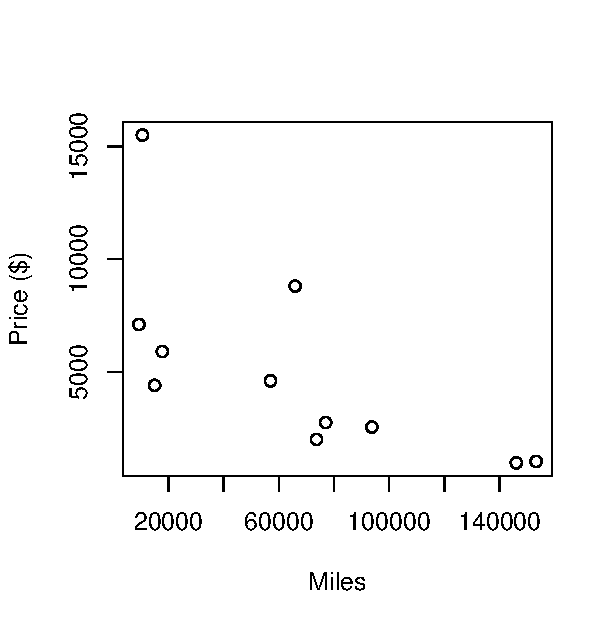
\includegraphics[width=7cm]{figure/LBL14a-1} 

}



% \end{figure}
\end{minipage}

\subsubsection{Problem:}

Based on the data, how much do I expect to get for a Saturn car that has been driven 60,000 miles?

Simple linear regression is a data analysis technique that tries to find a \textit{linear} pattern in the data.  We then use this line for prediction.

Notice that the points seem to fall around a \textit{straight line} sloping downwards.  Can you draw this line?  We will discuss one way to do this, called the \textit{least squares} (LS) method.  For now, suppose that the LS line has already been computed (we will do this later).  The LS line is overlayed on the scatterplot looks like Figure 14.1.

\begin{figure}[ht]
\centering
\caption{Least Squares (LS) Regression Line is overlayed on Scatterplot}


{\centering 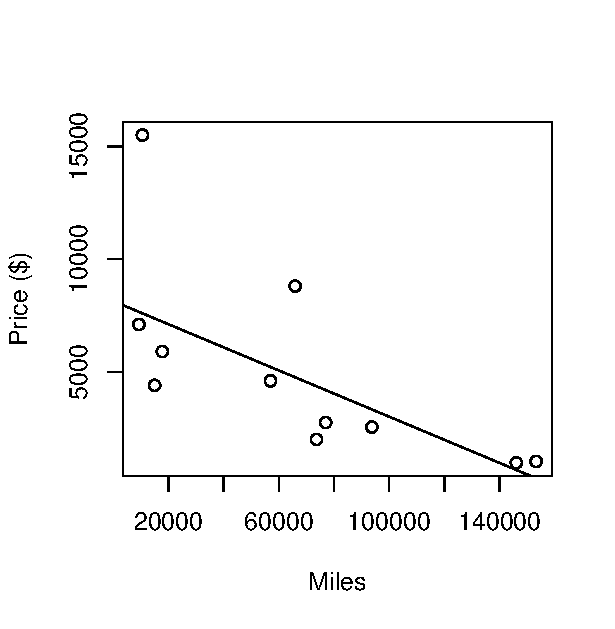
\includegraphics[width=8cm]{figure/LBL14b-1} 

}



\end{figure}

The formula for this line, in the form $Y= a + bX$,  is 

\begin{equation*}
  \texttt{Predicted Price} = 8136 + (-0.05127)(\texttt{Miles})
\end{equation*}

The \textit{slope} of the line is -0.05127, which means that predicted Price tends to drop 5 cents for every additional mile driven, or about \$512.70 for every 10,000 miles. The \textit{Y-intercept} of the line is \$ 8136; this should not be interpreted as the predicted price of a car with 0 mileage because the range of the data does not include cars with 0 miles.  

We can now use the line to predict the selling price of a car with 60000 miles.  What is the height or Y value of the line at $X = 60000$?  The answer is

\begin{equation*}
  \texttt{Predicted Price} = 8136 + (-0.05127)(60000) = \$5059.80
\end{equation*}

or about \$5000 or \$5100 or so.

\section{Calculating the Least Squares Regression Line}

One way to calculate the regression line is to use these five statistics:

$$ \bar{X}, S_{\bar{X}}, \bar{Y}, S_{\bar{Y}}, \texttt{ and } r  $$

(i.e., the mean and SD of $X$, the mean and SD of $Y$, and the correlation between $X$ and $Y$.)

\begin{center}
\fbox{\parbox{14cm}{
The least square regression line is given by the equation

\begin{equation*}
  \texttt{Predicted} = a + b X
\end{equation*}

where the slope $b$ and the intercept $a$ are calculated as 

\begin{eqnarray}
  b &=& r \frac{S_y}{S_x} \\
  a &=& \bar{Y} - b \bar{X}  \nonumber \\
\end{eqnarray}
}}
\end{center}

Next, we'll perform the calculations for the Saturn Price data. 

\begin{table}[ht]
\centering 
\begin{tabular}{@{} c rr @{}} \hline 
Car & Miles & Price (\$) \\ \hline
1 & 9300 & 7100 \\
2 & 10565 & 15500 \\
3 & 15000 & 4400 \\
4 & 15000 & 4400 \\
5 & 17764 & 5900 \\
6 & 57000 & 4600 \\
7 & 65940 & 8800 \\
8 & 73676 & 2000 \\
9 & 77006 & 2750 \\
10 & 93739 & 2550 \\
11 & 146088 & 960 \\
12 & 153260 & 1025 \\ \hline
Average & 61195 & 4999 \\
SD  & 50989 & 4079 \\
$r$ & \multicolumn{2}{c}{-0.641} \\ \hline
\end{tabular}
\end{table}

Using the formulas for slope and intercept in equation (14.1 and 14.2)

\begin{eqnarray*}
b &=& r \frac{S_y}{S_x} = -0.641 \frac{4079}{50989} = -0.05127 \\
a &=& \bar{Y} - b \bar{X} = 4999 - (-0.05127)(61195) = 8136  \\
\end{eqnarray*}

so that the regression line is

\begin{equation*}
PREDICTED = a + b X = 8136 + (-0.05127) X
\end{equation*}

In terms of the original variable names, the regression line is

\begin{equation*}
  \texttt{Predicted Price} = 8136 + (-0.05127) \texttt{Miles} 
\end{equation*}

\section{More on Simple Regression}

Why is this called the least squares line?  The answer is best shown by example.

\begin{table}[ht]


\centering 
\begin{tabular}{@{} c rrrc @{}} \hline 
Car & Miles & Price (\$) & PRED & RES = Y - PRED    \\ \hline
1 & 9300 & 7100 & 7659.35 & -559.35 \\
2 & 10565 & 15500 & 7594.49 & 7905.51 \\
3 & 15000 & 4400 & 7367.11 & -2967.11 \\
4 & 15000 & 4400 & 7367.11 & -2967.11 \\
5 & 17764 & 5900 & 7225.41 & -1325.41 \\
6 & 57000 & 4600 & 5213.82 & -613.82 \\
7 & 65940 & 8800 & 4755.47 & 4044.53 \\
8 & 73676 & 2000 & 4358.85 & -2358.85 \\
9 & 77006 & 2750 & 4188.13 & -1438.13 \\
10 & 93739 & 2550 & 3330.24 & -780.24 \\
11 & 146088 & 960 & 646.36 & 313.64 \\
12 & 153260 & 1025 & 278.66 & 746.34 \\ \hline
\end{tabular}
\end{table}

The first car has $Miles = 9300$.  What is its predicted price?  The predicted value is 

\begin{equation*}
  \texttt{Predicted Price} = 8136 + (-0.05127)(9300) = 7659.35
\end{equation*}

This predicted value missed the actual selling price $Y = 7100$.  By how much? By

\begin{equation*}
  \texttt{Residual} = 7100 + 7659.35 = -559.35
\end{equation*}

The negative value means actual value is too low.  This difference is called the residual.  

Small residuals (ignoring the sign) are good because this means the prediction was close  (Car 1 above was predicted well, but Car 2 was not -- the selling price is almost double what was predicted).  Therefore, a prediction line is good if it gives residuals that are as small as possible.  

\begin{center}
\fbox{\parbox{9cm}{
The sum of squared residuals is 
$$ SSE = (-559.35)^2 + \cdots + (746.34)^2 = 107805718.50 $$
}}
\end{center}

and is a measure of `overall size' of the residuals.  In the Saturn Price data, \\
$SSE =  107,805,718$.

\begin{center}
\fbox{\parbox{8cm}{
The least square line given by (14.1) will have a smaller SSE than any other straight line.
}}
\end{center}

This means that if you use any other intercept and slope combination besides $(a,b) = (8136,.05127)$, the new set of predicted values and residuals will give an SSE that is larger than, or at best equal to 107,805,718. 

\section{A 95\% Confidence Interval for Slope}

Is there a linear relationship between X and Y?  It seems obvious that selling price (Y) responds to a car's mileage (X), but in science, relationships are often not too obvious and need confirmation by data.  For example, does an individual's systolic blood pressure (Y) tend to increase with their cholesterol level (X)?   Is there a relationship between one's total number of years of education (X) and income (Y)?  In this section, we will investigate the strength of linear relationships by looking at the slope estimate.  Since the slope represents how much Y responds to changes in the X-value, we will calculate a 95\% confidence interval for the slope, and examine whether it excludes 0.  If it does, then we can rule out the likelihood that the slope is 0.  Thus, we conclude that there is a significant linear relationship between $X$ and $Y$.

We start by stating the formula for standard error:




% The correlation is a common and useful statistics.  It is a single number from $-1$ to $+1$ that indicates the strength of the relationship between the two variables.  If the number is between $-0.3$ and $+0.3 $, then we will say that the relationship is weak or non-existent. Otherwise, we will say that the relationship is either moderate or strong.  By the way, the closer we are to a $-1$ or a $+1$ the stronger the relationship.   The following example shows us how to interpret the results.
% 
% \subsection{Example 1}
% 
% Let's hypothesize that height of a male  affects the male's self-esteem.  We probably don't need to be concerned about the direction of causality; it is  unlikely that self-esteem causes a person's height.  We select a random sample of twenty males because we know that male heights are different from female heights.  By not using females heights  will simplify  the analysis.
% 
% \begin{minipage}[ht]{5cm}
% 
% {\small{
%  \begin{tabular}{@{} ccc @{}} \hline % Column formatting, @{} suppresses leading/trailing space
%      %  & \multicolumn{3}{c}{Category } \\ \hline
%      % \cmidrule(r){1-2} % Partial rule. (r) trims the line a little bit on the right; (l) & (lr) also possible
% Person & Height & Self.esteem \\ \hline
% 1 & 1.73 & 4.11 \\
% 2 & 1.81 & 4.62 \\
% 3 & 1.57 & 3.83 \\
% 4 & 1.91 & 4.44 \\
% 5	& 1.47 & 3.25 \\
% 6	& 1.52 & 3.16 \\
% 7	& 1.71 & 3.87 \\
% 8	& 1.73 & 4.18 \\
% 9	& 1.81 & 4.39 \\
% 10 & 1.75 & 3.70 \\
% 11 & 1.73 & 3.51 \\
% 12 & 1.71 & 3.22 \\
% 13 & 1.61 & 3.73 \\
% 14 & 1.57 & 3.34 \\
% 15 & 1.52 & 3.45 \\
% 16 & 1.61 & 4.06 \\
% 17 & 1.65 & 4.17 \\
% 18 & 1.71 & 3.89 \\
% 19 & 1.61 & 3.40 \\
% 20 & 1.55 &3.61 \\ \hline
% \end{tabular} }}
% 
% \end{minipage} \hfill
% \begin{minipage}[ht]{11cm}
% 
% \centering
% 
% Self Esteem by Height
% 
% <<f12_1, echo=FALSE, fig.pos="ht", fig.align="center", fig.width=3.5, fig.height=3.5, fig.path="chapters/Chapter_12/figure/">>=
%   dt12_1 <- read.csv("data/esteem.csv",header=TRUE)
%   plot( dt12_1$Self.esteem ~ dt12_1$Height.m, xlab="Height", ylab="Self Esteem")
%   lm_1 <- lm( dt12_1$Self.esteem ~ dt12_1$Height.m )
%   abline(lm_1)
% @
% 
% \end{minipage}
% 
% % \subsubsection{Scatter plot}
% 
% 
% As we review the scatter plot, we see that the direction of the relationship is positive, (i.e., as height increases, self-esteem increases).
% 
% Based on the above graphic, there appears to be a relationship between the two variables -- height and self-esteem.  But is this relationship real?  We will use the five-step model to confirm our initial assumption.
% 
% %\begin{itemize}
% %\item
% {\textbf{Step 1.}}  Making Assumptions and Meeting Test Requirements.
% 
% % Requires the booktabs if the memoir class is not being used
% \begin{table}[htbp]
%    \centering
%     \caption{Model Assumptions }
%    %\topcaption{Table captions are better up top} % requires the topcapt package
%    \begin{tabular}{@{} rl @{}} \hline % Column formatting, @{} suppresses leading/trailing space
%       % \multicolumn{2}{c}{Item} \\
%       % \cmidrule(r){1-2} % Partial rule. (r) trims the line a little bit on the right; (l) & (lr) also possible
%       1& Random sampling  \\
%       2      & Levels of Measurement are interval-ratio \\
%       3     & Bivariate normal distribution \\
%       4    & Linear relationship \\  \index{linear relationship}
%       5   & The variance of $Y$ scores is uniform for all $X$ values. \\
%       6  & Normality of residuals \\ \hline
%    \end{tabular}
%    \label{tab:t12_1}
% \end{table}
% 
% %\item
% {\textbf{Step 2.}}  State the Hypotheses. \\
%  $H_0: \rho = 0$ (there is no relationship between height and self-esteem) \\
%  $H_a: \rho \neq 0$  ($\rho$ represents the population \textbf{correlation coefficient}.)
% 
% % \item
%  {\textbf{Step 3.}}  Selecting the Sampling Distribution and Establishing the Critical Region.
% 
% 
%  % Requires the booktabs if the memoir class is not being used
% \begin{table}[htbp]
%    \centering
%    \caption{Components of correlation }
%    %\topcaption{Table captions are better up top} % requires the topcapt package
%    \begin{tabular}{@{} rcl @{}} \hline % Column formatting, @{} suppresses leading/trailing space
%       % \multicolumn{2}{c}{Item} \\
%       % \cmidrule(r){1-2} % Partial rule. (r) trims the line a little bit on the right; (l) & (lr) also possible
%       Sampling Distribution & = & t-distribution \\
%       Alpha $(\alpha)$ & = & 0.05 (two-tailed) \\
%       Degrees of Freedom  & = & $ n - 2 = 20 - 2 = 18 $  \\
%       $t_{critical}$ & = & 2.10 \\ \hline
%    \end{tabular}
%    \label{tab:t12_2}
% \end{table}
% 
% %\item
% {\textbf{Step 4.}}  Computing the Test Statistic.
% 
% The test statistic is computed by the following equation:
% 
% \begin{align*}
% t_{obtained} &= r \sqrt{ \frac{n - 2}{1 - r^2}} \\
%               &= 0.721 \sqrt{ \frac{20 - 2}{1 - 0.721^2}} \\
%               &= 4.4145 \\
% \end{align*}
% 
% From figure \ref{fig:f12_2} on page \pageref{fig:f12_2} (MINITAB printout), we find Pearson Correlation coefficient, $r = 0.721$.  In step 4, we see the test statistic ($t_{obtained}$) is equal to 4.41.
% 
%   \begin{figure}[ht]
%     \centering
%     \caption{MINITAB Correlation Analysis}
%     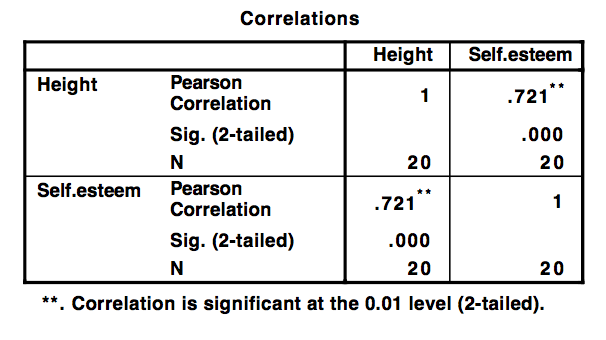
\includegraphics[width=10cm]{chapters/Chapter_12/ext_figure/zCorrA.png} % requires the graphicx package
%     \label{fig:f12_2}
%  \end{figure}
% 
% %\item
% {\textbf{Step 5:}} Deciding and Interpreting the Results of the Test
% 
% Since the $t_{obtained}$ (test statistic) is greater than the $t_{critical}$ value ($ 4.41 > 2.10 $), we reject the null hypothesis.  Thus, we can say that there is a strong, positive relationship  between male height and male self-esteem.
% %\end{itemize}
% 
% % \pagebreak
% \section{What is Linear Regression?}  \index{linear regression}
% 
% Regression analysis is a method that we use when the explanatory and response variables are both numeric, i.e., interval-ratio variables, for example, weights, heights, volumes, and temperature.  The easiest way of knowing if the regression is the appropriate method is to see a scatter plot of the data.  The researcher will choose the linear regression model if there is an apparent (linear) relationship.  Let's examine an example that will help explain the process.
% 
% Let's consider the relationship between the percent change of city population growth  from 2000 and 2008 and the number of annual car thefts.  As a researcher, we review the level of measurement and find that both variables are interval-ratio.  So we consider using the scatter plot.  It has two dimensions, the x-axis which is the explanatory (X) variable and the y-axis which is the response (Y) variable that we want to predict.
% 
% \begin{minipage}[ht]{5cm}
% 
% \centering
% {\small{
%    \begin{tabular}{@{} cc @{}} \hline % Column formatting, @{} suppresses leading/trailing space
%      %  & \multicolumn{3}{c}{Category } \\ \hline
%      % \cmidrule(r){1-2} % Partial rule. (r) trims the line a little bit on the right; (l) & (lr) also possible
%      Growth & Car.theft \\ \hline
%      9.8 & 118 \\
%      5.7 & 204 \\
%      1.3 & 294 \\
%      2.7 & 163 \\
%      26.8 & 764 \\
%      3.4 & 95 \\
%      16.8 & 392 \\
%      11.2 & 581 \\
%      8.6 & 601 \\
%      2.8 & 144 \\ \hline
%    \end{tabular}
% }}
% 
%   \end{minipage} \hfill
% \begin{minipage}[ht]{10cm}
% 
% \centering
% 
% Figure: 12.3, Car Theft by Growth
% 
% <<label=f12_3, echo=FALSE, fig.pos="ht", fig.align="center", fig.width=3.6, fig.height=3.6, fig.path="chapters/Chapter_12/figure/">>=
%   dt12_2 <- read.csv("data/EX12A.csv",header=TRUE)
%   plot( dt12_2$Car.theft ~ dt12_2$Growth, xlab="Growth", ylab="Car Theft")
%   lm_2 <- lm( dt12_2$Car.theft ~ dt12_2$Growth )
%   abline( lm_2 )
%   b_1 <- lm_2$coefficient[2]
%   b_0 <- lm_2$coefficient[1]
% 
%   xx_11 <- 20
%   xy_11 <- 0
% 
%   xy_22 <- b_0 + b_1 * 20
%   lines(c(xx_11,xy_11), c(xy_22, xy_22), col="red")
%   lines(c(xx_11, xx_11), c(xy_11, xy_22), col="red")
% @
% 
% \end{minipage}
% 
% \subsubsection{Interpreting Scatter Plot}
% 
% The pattern of points on the graph seems to indicate that  city growth (percent change from 2000 to 2008)  increases so does the number of auto thefts increase.  To demonstrate this pattern, we can draw a straight line that approximates the best fit for the points (See Figure 12.3).
% 
% \subsubsection{Does a Relationship Exist?}
% 
% The definition of an association states that the relationship between two variables will vary in the same direction either positive or negative.  As the \emph{X}-variable increases, the \emph{Y}-variable will increase (decrease if the direction is negative).  If a linear relationship exists between these two variables, then the best-fitted line through the points will not be parallel with the x-axis.
% % In other words, the \emph{X-Y} pair represents a point on the scatter plot.
% In a subsequent section, we will use a statistical method to test this hypothesis.
% 
% \subsubsection{How Strong is the association?}
% 
% The density around the fitted regression line assesses the strength of this relationship.  If the relationship is perfect, then the points of \emph{X - Y} will lie  on the fitted regression line.  Otherwise, the relationship becomes weaker when the data points are away from the fitted regression line.  What we are talking about here is the correlation coefficient.
% 
% From Figure \ref{fig:f12_4} on page \pageref{fig:f12_4} (MINITAB printout), we find Pearson Correlation coefficient, $r = 0.773$ indicating that we have a high correlation between city growth and car theft.  Note the arrow is pointing to the correlation coefficient.
% 
%   \begin{figure}[ht]
%     \centering
%     \caption{MINITAB Correlation Analysis}
%     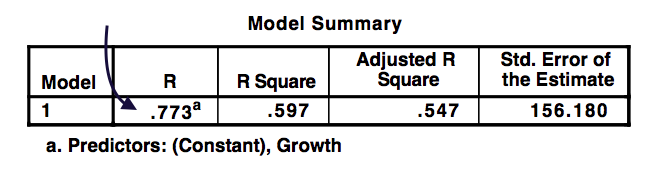
\includegraphics[width=11cm]{chapters/Chapter_12/ext_figure/zEX12corr.png} % requires the graphicx package
%     \label{fig:f12_4}
%  \end{figure}
% 
% \subsubsection{Predicting response variable using the scatter plot}
% 
% We can use the scatter plot for prediction.  To show this procedure, let's look at the relationship between city growth and annual car thefts illustrated in Figure 12.3.  Let's say that we want to predict the number of car thefts in a city that has grown by 20 percent from 2000 to 2008.  The predicted score on \emph{Y} (indicated by $\hat{Y}$) to discriminate between the predictions of \emph{Y} from the actual \emph{Y} scores.  First, we should locate 20 on the x-axis and then draw a straight line parallel with the y-axis and to the regression line.  From the regression line, draw another line that is parallel to the x-axis to the y-axis.  The predicted \emph{Y} ($\hat{Y}$) is found at the point where the line crosses the y-axis.  We predict that cities that have grown by 20 percent from 2000 to 2008, the number of car thefts would be around 600 per year.  Later, we will develop a model for making this prediction.
% 
% \subsubsection{The Regression Line}
% 
% Using the above method is crude because trying to fit a line through a cloud of points by using a free hand.  A mathematical method has been developed and implemented in many statistical programs, such as SPSS, MINITAB, SAS, R, etc., to solve this fundamental equation:
% 
% \begin{equation}
% Y = a + bX
% \end{equation}
% 
% \begin{align*}
% Y &= Dependent \hspace{1mm} Variable \\
% a &= Y \hspace{1mm} intercept \\  \index{intercept}
% b &= Slope \\  \index{slope}
% X &= Independent \hspace{1mm} Variable
% \end{align*}
% 
% \subsubsection{Determining the y-intercept (a)}
% 
% From the MINITAB output Figure \ref{fig:f12_5}, let's determine the y-intercept of this  problem.
% 
%   \begin{figure}[ht]
%     \centering
%     \caption{MINITAB Regression Analysis}
%     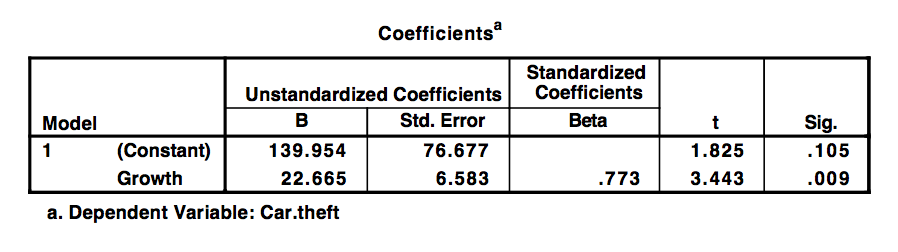
\includegraphics[width=11cm]{chapters/Chapter_12/ext_figure/zRegD.png} % requires the graphicx package
%     \label{fig:f12_5}
%  \end{figure}
% 
%  After reviewing Figure \ref{fig:f12_5}, we find column B and row (Constant) (a) is 139.954.  Our interpretation of the y-intercept is 139.954 when \emph{X} = 0.  Now keep this number in mind as we determine the slope because we will use these two numbers to predict the annual car theft based on the percent change that a city experienced from 2000 to 2008.
% 
% \subsubsection{Determine the slope (b) }
% 
% From the MINITAB output Figure \ref{fig:f12_5}, let's identify the slope of this  problem.
% 
% After reviewing Figure \ref{fig:f12_5}, we find column B and row Growth that the slope (b) is 22.665.  Our interpretation of the slope is that as the percentage change of the cities growth increases by 1 percent, the number of car thefts increases by 22.665 per year.  Let's evaluate the slope with the five step model.
% 
% \begin{itemize}
% \item {\textbf{Step 1.}}  Making Assumptions and Meeting Test Requirements.
% 
% % Requires the booktabs if the memoir class is not being used
% \begin{table}[htbp]
%    \centering
%     \caption{Model Assumptions}
%    %\topcaption{Table captions are better up top} % requires the topcapt package
%    \begin{tabular}{@{} rl @{}} \hline % Column formatting, @{} suppresses leading/trailing space
%       % \multicolumn{2}{c}{Item} \\
%       % \cmidrule(r){1-2} % Partial rule. (r) trims the line a little bit on the right; (l) & (lr) also possible
%       1 & Random sampling  \\
%       2       & Levels of Measurement are interval-ratio \\
%       3       & Bivariate normal distribution \\
%       4       & Linear relationship \\
%       5       & Variance of $Y$ scores is uniform for all $X$ values. \\
%       6       & Normality of residuals. \\ \hline
%    \end{tabular}
%    \label{tab:t12_3}
% \end{table}
% 
% \item {\textbf{Step 2.}}  State the Hypotheses. \\
%  $H_0: \beta = 0$ (there is no relationship between percent change of a city and car theft) \\
%  $H_a: \beta \neq 0$ (where $\beta$ represents the population \textbf{slope}.)
%  \item {\textbf{Step 3.}}  Selecting the Sampling Distribution and Establishing the Critical Region.
% 
% 
%  % Requires the booktabs if the memoir class is not being used
% \begin{table}[htbp]
%    \centering
%     \caption{Components of correlation}
%    %\topcaption{Table captions are better up top} % requires the topcapt package
%    \begin{tabular}{@{} rcl @{}} \hline % Column formatting, @{} suppresses leading/trailing space
%       % \multicolumn{2}{c}{Item} \\
%       % \cmidrule(r){1-2} % Partial rule. (r) trims the line a little bit on the right; (l) & (lr) also possible
%       Sampling Distribution & = & t-distribution \\
%       Alpha $(\alpha)$ & = & 0.05 (two-tailed) \\
%       Degrees of Freedom  & = & $ n - 2 = 10 - 2 = 8 $  \\
%       $t_{critical}$ & = & 2.3060 \\ \hline
%    \end{tabular}
%    \label{tab:t12_4}
% \end{table}
% 
% \item {\textbf{Step 4.}}  Determine the Test Statistic.
% 
% The test statistic is determined from  the following table.
% 
% From Figure \ref{fig:f12_6}, (MINITAB printout), we find the slope (b) = 22.665.  The test statistic $t$ is 3.443, from row Growth and column $t$.
% 
%   \begin{figure}[ht]
%     \centering
%     \caption{MINITAB Regression Analysis}
%     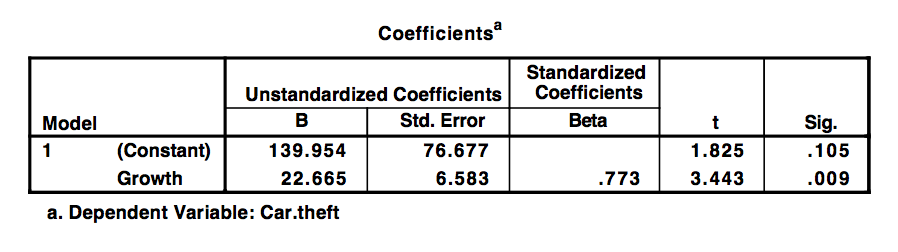
\includegraphics[width=11cm]{chapters/Chapter_12/ext_figure/zRegD.png} % requires the graphicx package
%     \label{fig:f12_6}
%  \end{figure}
% 
% \item {\textbf{Step 5:}} Making a Decision and Interpreting the Results of the Test
% 
% Since the $t_{obtained}$ (test statistic) is greater than the $t_{critical}$ value ($ 3.443 > 2.2060 $), we reject the null hypothesis. Thus we can interpret the slope by saying as the percent change in  city increases by one, the number of annual car thefts increases by 22.7.
% 
% \end{itemize}
% 
% \subsubsection{Prediction}
% 
% Now let's put it all together.  We have an equation.  We will use the same \emph{X}-value = 20 that we used when we used a graphical solution for this problem.
% 
% \begin{align*}
% \hat{Y} &= a + b(X) \\
% CarThefts &= 139.954 + 22.665(Growth) \\
%           &= 139.954 + 22.665(20) \\
%           &= 593.3
% \end{align*}
% 
% We can now say that a city that had percent change growth of 20 percent will have an estimated 593 automobiles stolen in one year.
% 
% \subsubsection{Interpreting the Regression}
% 
% What variables can she collect to predict the final exam score of an Introductory Statistics course?  Statistics instructors have been asking this question for a long time.  An instructor gathered,  (four explanatory variables (MT1, MT2, Proj, HW)), data from 64 of her statistics class students and did the following analysis.
% 
% \subsubsection{Descriptive Statistics}
% 
% Table \ref{tab:t12_5} reports the basic descriptive statistics for the variables.  The average final exam score is 156.1 with a score ranging  from 75 to 191.  The mean mid-term  test one score is 86.1 with a score ranging from 50 to 99.  As consultants, we should ask ourselves, what explanatory variables should we use to predict the final exam score.
% 
%  % Requires the booktabs if the memoir class is not being used
% \begin{table}[htbp]
%    \centering
%     \caption{Descriptive Statistics }
%    %\topcaption{Table captions are better up top} % requires the topcapt package
%    \begin{tabular}{@{} lccccc @{}} \hline % Column formatting, @{} suppresses leading/trailing space
%        &  \multicolumn{5}{c}{Descriptive Statistics} \\
%       % \cmidrule(r){1-2} % Partial rule. (r) trims the line a little bit on the right; (l) & (lr) also possible
%       Statistics & Final & MT1 & MT2 & Proj & HW \\ \hline
%       Mean & 156.1 & 86.1 & 74.2 & 10.1 & 72.3 \\
%       Standard deviation & 24.47 & 11.51 & 18.59 & 1.16 & 11.69 \\
%       N & 64 & 64 & 64 & 64 & 64 \\ \hline
%    \end{tabular}
%    \label{tab:t12_5}
% \end{table}
% 
% \begin{itemize}
% \item Where
%   \begin{itemize}
%   \samepage
%   \item Final --  Exam score
%   \samepage
%   \item MT1 -- Midterm exam one score
%   \samepage
%   \item MT2 -- Midterm exam two score
%   \samepage
%   \item Proj -- Project score
%   \samepage
%   \item HW -- Homework score
%   \samepage
%   \end{itemize}
% \end{itemize}
% 
% 
% \subsubsection{Correlation matrix}
% 
%  % Requires the booktabs if the memoir class is not being used
% \begin{table}[htbp]
%    \centering
%     \caption{Pearson Correlation Coefficient}
%    \begin{tabular}{@{} lccccc @{}} \hline % Column formatting, @{} suppresses leading/trailing space
%       % &  \multicolumn{5}{c}{Pearson Correlation} \\
%       % \cmidrule(r){1-2} % Partial rule. (r) trims the line a little bit on the right; (l) & (lr) also possible
%       Statistics & Final & MT1 & MT2 & Project & HW \\ \hline
%       Final & 1  \\
%       MT1   & \fbox{0.751} & 1 \\
%       MT2   & 0.543 & 0.454 & 1 \\
%       Proj & 0.087 & 0.101 & -0.032 & 1 \\
%       HW      & 0.273 & 0.301 & 0.218 & 0.093 & 1 \\ \hline
%    \end{tabular}
%    \label{tab:t12_6}
% \end{table}
% 
% After reviewing the correlation matrix (Table \ref{tab:t12_6}), we see that at the intersection of Final and MT1 has a correlation coefficient ($r = 0.751$) which is the largest number in the matrix.  This number tells us that we have a strong positive relationship between the mean final exam score and the mean mid-term exam one score.  The coefficient of determination ($r^2 = 0.564$) which tells us that the mid-term one score explains 56.4 percent of the variance in the final exam score.
% 
% \subsubsection{Scatter plot}  \index{scatter plot}
% 
% The next step in assessing an association between two interval-ratio variables is the scatter plot.  Figure \ref{fig:f12_7} displays the final exam scores on the vertical, \emph{Y}, axis, and the mid-term evaluation one score on the horizontal, \emph{X}, axis.
% 
% <<label=f12_7, echo=FALSE, fig.pos="ht", fig.align="center", fig.width=8, fig.height=8, fig.cap="Mid-term 1 Exam", out.width="6cm", fig.path="chapters/Chapter_12/figure/">>=
%   dt12_3 <- read.csv("data/grades.csv",header=TRUE)
%   plot( dt12_3$Final ~ dt12_3$MT1, xlab="Mid-Term 1 ", ylab="Final")
%   lm_3 <- lm( dt12_3$Final ~ dt12_3$MT1 )
%   abline( lm_3 )
%   b_1 <- lm_3$coefficient[2]
%   b_0 <- lm_3$coefficient[1]
% @
% 
% What can we say about the relationship?  The regression line is \emph{not} horizontal, so there is an association between these two variables.  The graph shows points scattered around the regression line, and we can see that we have a strong positive relationship.
% 
% \subsubsection{Regression Equation}  \index{regression equation}
% 
% The next step is to determine the regression equation.
% 
%   \begin{figure}[ht]
%     \centering
%     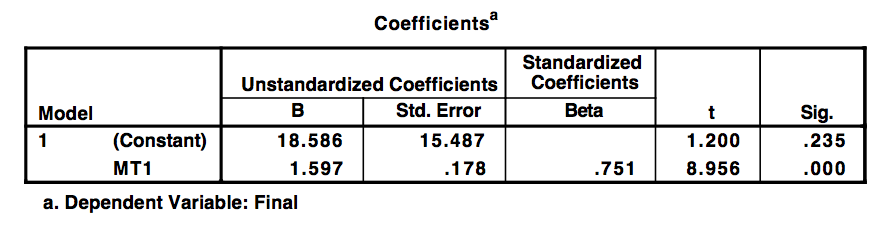
\includegraphics[width=12cm]{chapters/Chapter_12/ext_figure/zRegE.png} % requires the graphicx package
%     \caption{MINITAB Regression Analysis }
%     \label{fig:f12_8}
%  \end{figure}
% 
% After reviewing Figure \ref{fig:f12_8}, we find the \emph{Y}-intercept (\emph{a}) is 18.586, row (constant) and column B.  The slope (\emph{b}) is 1.597, row MT1 and column B.
% 
% \begin{align*}
%     Y &= a + bX \\
% Final &= 18.586 + 1.597(MT1)
% \end{align*}
% 
% The interpretation of the slope is as mid-term one exam scores increase by one unit, the final exam score increase by 1.597 points.
% 
% \subsubsection{Diagnostics}
% 
% \begin{itemize}
% \item Coefficient of determination:  \index{coefficient determination}
%   \begin{itemize}
%   \item $r^2 = \frac{explained Variation}{total Variation}$
%   \item We measure the explained variation from the average of the \emph{Y}-variable to the predicted \emph{Y}-variable.
%   \item We compute the unexplained variation from the observed \emph{Y}-variable to the predicted \emph{Y}-variable.
%   \item We determine the total change from the observed \emph{Y}-variable to the average of the \emph{Y}-variable.
%   \end{itemize}
% 
% \item There is one other thing that we should look at --  residuals.
%   \begin{itemize}
%   \item For each data point, we should compute the difference:
% 
%   \begin{equation}
%   Residual_i =  observedValue_i - predictedValue_i
%   \end{equation}
% 
% 
%   \item The histogram of the residuals should be  bell-shaped as in Figure \ref{fig:f12_9}.
% 
% 
% %\begin{minipage}[ht]{6.5cm}
% 
%   <<label=f12_9,  echo=FALSE, fig.pos="ht", fig.align="center", fig.width=8, fig.height=8, fig.cap="Histogram of Residuals", out.width="6cm", fig.path="chapters/Chapter_12/figure/">>=
%   hist(lm_3$residuals)
%   @
% 
% %\end{minipage} \hfill
% %\begin{minipage}[ht]{6.5cm}
% 
%   <<label=f12_10, echo=FALSE, fig.pos="ht", fig.align="center", fig.width=8, fig.height=8, fig.cap="Residual Plot", out.width="6cm", fig.path="chapters/Chapter_12/figure/">>=
% 
%   plot( lm_3$residuals ~ lm_3$fitted.values, xlab="Final -- fitted values ", ylab="Residuals")
%   abline( 0,0 )
% @
% 
% %\end{minipage}
% 
%   \item Let's look at Figure \ref{fig:f12_9}.  Here we can draw a nearly normal-shaped curve over the histogram.
%   \end{itemize}
% 
% \item Another assumption that we need to consider is homoscedasticity, i.e.,  \index{homoscedasticity} is the variance of \emph{Y} scores uniform across all values of \emph{X}.
% 
%   \begin{itemize}
% 
%   \item Figure \ref{fig:f12_10} shows a pattern of points that is uniform.
% 
%   \end{itemize}
% 
% \end{itemize}
% 
% \subsubsection{Summary}
% 
% To conclude this analysis, the linear regression equation, the correlation coefficient, and coefficient of determination suggest that there exist a positive and strong relationship between the first mid-term exam score  and the final exam score.  The amount of unexplained variation (total variation - explained variation, i.e., 100 - 55 = 45) suggests that there may be other variables besides first mid-term exam that have a significant influence on the final exam score.
% 
% We should note one limitation of the simple linear regression.  First correlation is not the same as causation.  In other words, two variables that are highly correlated does not necessarily suggest that there is a causal relationship.  We could take these results to support the proposition that higher mid-term exam scores lead to higher final exam scores, the mere existence of a relationship -- even a strong connection in the direction predicted by the theory -- does not prove that one variable causes the other.
% 
% \section{Key Words}
% 
% \colorbox{lgray}{\parbox{15cm}{
% \begin{minipage}[ht]{6cm}
% \begin{itemize}
% \item Bivariate normal distribution
% \item Coefficient of discrimination
% \item Correlation matrix
% \item Explained variation
% \item Homoscedasticity
% \item Linear relationship
% \item Pearson's r
% \end{itemize}
% 
% \end{minipage} \hfill
% \begin{minipage}[ht]{6cm}
% \begin{itemize}
% \item Regression line
% \item Scatter plot
% \item Slope
% \item Total variation
% \item Unexplained variation
% \item \emph{Y}-intercept
% \item $\hat{Y}$
% \end{itemize}
% \end{minipage}
% }}
% 
% \twocolumn
% \section{Exercises}
% 
% \begin{exercises}
% 
%   \begin{exercise} % 1
% 
% <<label=f12_11, echo=FALSE, fig.pos="ht", fig.align="center", fig.width=3, fig.height=3, fig.cap="Beers vs. BAC", fig.path="chapters/Chapter_12/figure/">>=
%      dt12_4 <- read.csv("data/beers.csv",header=TRUE)
%      plot( dt12_4$BAC ~ dt12_4$NB, xlab="NB", ylab="BAC")
%      lm_4 <- lm( dt12_4$BAC ~ dt12_4$NB )
%      abline( lm_4 )
%      b_1 <- lm_4$coefficient[2]
%      b_0 <- lm_4$coefficient[1]
%      rho1 <- cor(dt12_4$BAC, dt12_4$NB)
%      rho2 <- rho1^2
% @
% 
% The next three exercises use this scenario.  How well does the number of beers a student drinks predict his or her Blood Alcohol Content (BAC)? Sociology researchers, at Ohio State University, wanted to know if there is a relationship between the amount of beer consumed and BAC. The researchers assigned the number of cans of beer to each student. After each student had consumed the assigned number of beers,  thirty minutes later, an officer of the law measured the students BAC. \citep{OSU2016}  One student drank nine beers.  You see from the scatter plot \ref{fig:f12_11} that his BAC was about
% 
%     \begin{enumerate}
%     \item 0.014
%     \item 0.14
%     \item 1.4
%     \item 14
%     % \item 140
%     \end{enumerate}
% 
%     \framebox[5cm][l]{ Answer: }
% 
%   \end{exercise}
%   \begin{solution}  % 1
% 
%      $ BAC = -0.012 + 0.017 (9) = 0.14 $
%   \end{solution}
% 
%   \begin{exercise} % 2
% 
% Use the information from \\ exercise 1.  The scatterplot \ref{fig:f12_11} on page \pageref{fig:f12_11} shows
% 
%       \begin{enumerate}
%       \item a weak negative relationship.
%       \item a moderately high negative correlation.
%       \item almost no connection.
%       \item a small positive correlation.
%       \item a moderately high positive straight-line relationship between some beers and BAC.
%       \end{enumerate}
% 
%     \framebox[7cm][l]{ Answer: }
%   \end{exercise}
%   % \begin{solution}  % 2
%   %
%   %   A moderately strong positive straight-line relationship between number of beers and BAC.
%   % \end{solution}
% 
%   \begin{exercise} % 3
% 
% Use the information from \\ exercise 1.  A plausible value of the correlation between number of beers and blood alcohol content, based on the scatterplot, is
% 
%       \begin{enumerate}
%       \item $r =  -0.875$
%       \item $r =  -0.765$
%       \item $r$ close to 0
%       \item $r = 0.765$
%       \item $r = 0.875$
%       \end{enumerate}
% 
%     \framebox[7cm][l]{ Answer: }
%     \end{exercise}
%     \begin{solution}  % 3
% 
% The correllation coefficient is $r = rho1 = \sqrt{r^2 }$ where  $r^2$ is the coefficient of determination.
%     \end{solution}
% 
%   \begin{exercise} % 4
% 
% <<label=f12_14a, results="asis", echo=FALSE, fig.pos="ht", fig.align="center", fig.width=3, fig.height=3, fig.cap="Resp. Ht vs. Inc.", fig.path="chapters/Chapter_12/figure/">>=
% 
% dt12_5 <- read.csv("data/GSS2014.csv", header=TRUE)
%   ## dt12_5 <- read.csv("~/Desktop/GSS2014 copy.csv", header=TRUE)
% x12_1 <- cbind( dt12_5$HEIGHT, dt12_5$rincom06 )            ## select only the respondent's height and income
% x12_2 <- x12_1[ (dt12_5$HEIGHT > 0 & dt12_5$HEIGHT < 98) &
% 						  (dt12_5$rincom06 > 0 & dt12_5$rincom06 < 26),  ]          ## select only valid data
% nrw12 <- length( x12_2[ , 1] )
% x12_3 <- x12_2[ sample( 1:nrw12, size= 100, replace = TRUE),  ]
% Height <- x12_3[,1]
% Income <- x12_3[,2]
% plot(Height, Income, xlab="Height(inch)", ylab="Income(K dollars)", main="Plot of Ht vs. Inc." )
% 
% cor12 <- cor(Income, Height)
% cor12p <- sprintf("%.4f", cor12)
% rSq   <- cor12^2
% 
% m12 <- lm(Income ~ Height)
% abline(m12)
% 
% @
% 
% STEP 1: In the next six tasks use Figure \ref{fig:f12_14a}, we will use the data from \\ GSS2014 in this exercise.  We have been asked to examine the relationship between a person's height and a person's income.  Here we have {\textit{income}} which is an  interval-ratio type of variable while {\textit{height}} is also an interval-ratio type of variable.  These types of variables require that we use a Simple Linear Regression (SLR) analysis.  So step 1 in the process of analysis \emph{is to choose} the independent and dependent variables.  Note: In the GSS2014 dataset, {\textit{height}} is known as HEIGHT and {\textit{income}} is known as rincom06.  The correlation coefficient is cor12p.
% 
%     \framebox[7cm][l]{ Answer: }
%     \end{exercise}
%     % \begin{solution}  % 4
%     %    The independent variable is HEIGHT and the dependent variable is rincom06.
%     % \end{solution}
% 
%   \begin{exercise} % 5
% 
% STEP 2: Using the information from exercise four, we must state the hypotheses about its relationship between {\textit{income}} and {\textit{height}}.  Based on our experience, how should we state our hypotheses?
% 
%     \framebox[7cm][l]{ Answer: }
%     \end{exercise}
%     \begin{solution}  % 5
% 
%        $H_0: \beta = 0" vs. $H_1: \beta \ne 0$
%     \end{solution}
% 
%   \begin{exercise} % 6
% 
% STEP 3: Using the information from exercise four, determine the coefficient of determination. \index{coefficient of determination}  Recall that this value is also referred to as r-squared.
% 
%     \framebox[7cm][l]{ Answer: }
%     \end{exercise}
%     % \begin{solution}  % 6
%     %
%     %    The correlation coefficient between the respondent's height and income is rSq
%     % \end{solution}
% 
%   \begin{exercise} % 7
% 
% STEP 4: Using the information from exercise four, record the independent, dependent variables, and the correlation coefficient.  Record the requested information in table \ref{tab:t12_7} on page \pageref{tab:t12_7}.
% 
%   %  \framebox[8cm][l]{ Answer: }
%     \end{exercise}
%     \begin{solution}  % 7
% 
%     \begin{table}[ht]
%     \centering
%     \begin{tabular}{lr} \hline
%         &  \multicolumn{1}{c}{Independent} \\ \hline
%     Dep. Var. & 1. height \\ \hline
%     1. income  &   cor12 \\ \hline
%     \end{tabular}
%     \end{table}
%     \end{solution}
% 
%       \begin{exercise} % 8
% 
% STEP 5: Using the information from exercise four, describe the results of the independent variable.  Identify variables that we tested, their strength and direction of the relationship.  We should distinguish the relationship in general terms and refer the statistical value in parentheses.  Also not whether the hypotheses were supported.
% 
%     \framebox[7cm][l]{ Answer: }
% 
%     \end{exercise}
% %     \begin{solution}  % 8
% %
% % For a sample of 40 subjects, we tested the relationship between height and income.  We found a weak positive relationship using the correlation coefficient (cor12).  We then looked at the slope:  as {\textit{height}} increases by one inch, {\textit{income}} increases by m12$coefficients[2] with a p-value of
% %     \end{solution}
% 
%   \begin{exercise} % 9
% 
% STEP 1:  In the next six tasks, we will use a sample of 100 subjects from the GSS2014 data in this exercise.  We have been asked to examine the relationship between a person's income, age, and ``not married'' and a person's happiness.  Here we have variables which are the interval-ratio type of variable.  These types of variables require that we use a Simple Linear Regression (SLR) analysis table \ref{tbl12_15a} on page \pageref{tbl12_15a}.  So step 1 in the process of analysis is choosing independent and dependent variables.  Note: In the GSS2014 dataset, {\textit{happy (1)}} is known as GENERAL \\ HAPPINESS, {\textit{income06(2)}} is known as TOTAL FAMILY INCOME, {\textit{age(3)}} is known as AGE OF RESPONDENT, and {\textit{absingle(4)}} is known as \\ NOT MARRIED.
% 
% <<f12_15, results="asis", echo=FALSE, fig.pos="ht", fig.align="center", fig.width=2.5, fig.height=2.5, fig.cap="Respondent's Height vs. Income", fig.path="chapters/Chapter_12/figure/">>=
% 
% x12_9 <- cbind( dt12_5$happy, dt12_5$age, dt12_5$income06, dt12_5$absingle )            ## select only the respondent's height and income
% x12_10 <- x12_9[ (dt12_5$happy > 0 & dt12_5$happy < 8) &
% 						  (dt12_5$income06 > 0 & dt12_5$income06 < 26) &
% 						  (dt12_5$age  > 0) & (dt12_5$age < 98) &
% 						  (dt12_5$absingle > 0) & (dt12_5$absingle < 8),  ]  ## select only valid data
% nrw4 <- length( x12_10[ , 1] )
% x12_11 <- x12_10[ sample( 1:nrw4, size= 100, replace = TRUE),  ]
% Happiness  <- x12_11[,1]
% Age        <- x12_11[,2]
% Income     <- x12_11[,3]
% NotMarried <- x12_11[,4]
% 
%   cor13 <- cor(x12_11)
% 
%   print(xtable(cor13, caption='Correlation Coefficients Table', label="tab:12_15b"), caption.placement="top")
% 
%   m13 <- lm( Happiness ~  Age + Income + NotMarried )
% @
% 
% What are the dependent and independent variables?
% 
% 
%     \framebox[7cm][l]{ Answer: }
%     \end{exercise}
%     \begin{solution}  % 9
% 
%        The independent variable is income, age, and absingle and the dependent variable is happiness.
%     \end{solution}
% 
%   \begin{exercise} % 10
% 
% STEP 2: Using the information from exercise nine, we must state the hypotheses about its relationship between {\textit{Happiness}}, {\textit{income}},  {\textit{age}}, {\textit{NotMarried}}.  Based on our experience, how should we state our hypotheses?
% 
%     \framebox[7cm][l]{ Answer: }
% 
%     \end{exercise}
%     % \begin{solution}  % 10
%     %
%     %    $H_0: \beta_1 = \beta_2 = \beta_3 = 0$ \\
%     %    $H_1:$ at least one slope is not equal zero. \\
%     %    where $\beta_1$ is the slope for Happiness and Income,  $\beta_2$ is the slope for Happiness and Age and $\beta_3$ is         the slope for Happiness and single.
%     % \end{solution}
% 
%   \begin{exercise} % 11
% 
% STEP 3: Using the information from exercise nine, determine the coefficient of determination.
% 
%     \framebox[7cm][l]{ Answer: }
%     \end{exercise}
%     \begin{solution}  % 11
% 
%        Read the results from the computer generated output.
%     \end{solution}
% 
%   \begin{exercise} % 12
% 
% STEP 4: Using the information from exercise nine, record the independent, dependent variables, and the correlation coefficients information onto table \ref{tab:t12_12} on page \pageref{tab:t12_12}.
% 
%   %  \framebox[7cm][l]{ Answer: }
%     \end{exercise}
%     % \begin{solution}  % 12
%     %
%     %   The results are in the table.
%     % \end{solution}
% 
%   \begin{exercise} % 13
% 
% STEP 5:  Using the information from exercise nine, record the independent, dependent variables, and the correlation coefficients.
% 
%   %  \framebox[8cm][l]{ Answer: }
%     \end{exercise}
%     \begin{solution}  % 13
% 
%   The results are in the table.
%     \end{solution}
% 
%   \begin{exercise} % 14
% 
% STEP 1: A mail-order catalog business selling supplies for computers manages a centralized warehouse for disemination of products that customers ordered.  The  leadership team is examining the process of distribution from the warehouse and is considering the factors that affect the overall cost of operation.  It now has a small handling fee for each order, regardless the amount of the order.  Over the past 24 months, the team collected data such as the \emph{distribution cost(1)} (\$000), \emph{Sales(2)} (\$000), and the \emph{number of orders received(3)}.
% 
% % STEP 1:  In the next six tasks, we will use all of the data from GSS2014 in this exercise.  We have been asked to examine the relationship between a person's income, age, and ``not married'' and a person's happiness.  Here we have variables which are  interval-ratio type of variable.  These types of variables require that we use a Simple Linear Regression (SLR) analysis.  So step 1 in the process of analysis is choosing independent and dependent variables.  Note: In the GSS2014 dataset, {\textit{happy}} is known as GENERAL HAPPINESS, {\textit{income06}} is known as TOTAL FAMILY INCOME, {\textit{age}} is known as AGE OF RESPONDENT, and {\textit{absingle}} is known as NOT MARRIED.
% 
% <<f12_16, results="asis", echo=FALSE, fig.pos="ht", fig.align="center", fig.width=3.5, fig.height=3.5, fig.cap="Respondent's Height vs. Income", fig.path="chapters/Chapter_12/figure/">>=
% 
%   ## dt12_5 <- read.csv("~/github/STAT1600book/chapters/Chapter_12/data/warehouseCost.csv", header=TRUE)
%   dt12_5 <- read.csv("data/warehouseCost.csv", header=TRUE)
%   x12_10 <- cbind(dt12_5$DistCost, dt12_5$Sales, dt12_5$Orders)
% 
%   nrw4 <- length( x12_10[ , 1] )
% ## x12_11 <- x12_10[ sample( 1:nrw4, size= 100, replace = TRUE),  ]
%   DistCost <- x12_10[,1]
%   Sales    <- x12_10[,2]
%   Orders   <- x12_10[,3]
% 
%   cor14 <- cor(x12_10 )
% 
%   print(xtable(cor14, caption="Correlation Coefficient", label="tab: t12_16a"), caption.placement="top")
% 
%   m14 <- lm( DistCost ~ Sales + Orders )
%   aov16 <- aov(m14)
% @
% 
% What are the dependent and independent variables?
% 
%     \framebox[7cm][l]{ Answer: }
% 
%     \end{exercise}
%     % \begin{solution}  % 14
%     %
%     %    The independent variables are  Sales and  Orders and the dependent variable is DistCost.
%     % \end{solution}
% 
% 
%   \begin{exercise} % 15
% 
% STEP 2: Using the information from exercise 14, we must state the hypotheses about its relationship between {\textit{DistCost}}, \\ {\textit{Sales}}, and {\textit{Orders}}.  Based on our experience, how should we state our hypotheses?
% 
%     \framebox[7cm][l]{ Answer: }
%     \end{exercise}
%     \begin{solution}  % 15
% 
%        $H_0: \beta_1 = \beta_2 =  = 0$ \\
%        $H_1:$ at least one slope is not equal zero. \\
%        where $\beta_1$ is the slope for DistCost and Sales,  $\beta_2$ is the slope for DistCost and Orders
%     \end{solution}
% 
%   \begin{exercise} % 16
% 
% STEP 3: Using the information from exercise 14, Table \ref{tab:t12_16b} determine the coefficient of determination.
% 
% 
%     \framebox[7cm][l]{ Answer: }
%     \end{exercise}
%     % \begin{solution}  % 16
%     %
%     %    Read the results from the computer generated output.
%     % \end{solution}
% 
%   \begin{exercise} % 17
% 
%  STEP 4: Using the information from exercise nine, record the independent, dependent variables, and the correlation coefficients.
% 
% 
%   %  \framebox[7cm][l]{ Answer: }
%     \end{exercise}
%     \begin{solution}  % 17
% 
%       The results are in the table.
%     \end{solution}
% 
%   \begin{exercise} % 18
% 
% STEP 5:  Using the information from exercise nine, record the independent, dependent variables, and the correlation coefficients.
% 
%   %  \framebox[7cm][l]{ Answer: }
%   \end{exercise}
%   % \begin{solution}  % 18
%   %
%   % The results are in the table.
%   %   \end{solution}
% 
% \end{exercises}
% \onecolumn
% 
% 
% % <<label=lbl12_5a, results='asis', echo=FALSE>>=
% %   print(xtable(m12, caption='Coefficients', label="tab:12-7"), caption.placement="top")
% %
% % @
% 
% \begin{table}[ht]
%     \centering
%     \caption{exercise \# 7}
%     \begin{tabular}{lr} \hline
%         &  \multicolumn{1}{c}{Independent} \\ \hline
% 
%     Dep. Var. & 1. \underline{\phantom{xxxxxxxxxxxx}}      \\ \hline
%     1. \underline{\phantom{xxxxxxxxxxxx}}  &  \underline{\phantom{xxxxxxxxxxxx}}       \\ \hline
% 
%     \end{tabular}
%     \label{tab:t12_7}
% \end{table}
% 
% <<label=lbl12_15a, results='asis', echo=FALSE>>=
%   print(xtable(summary(m13), caption='Regression Analysis: Happiness vs. Age, Income, and Marital Status', label="tbl12_15a"), caption.placement="top")
% @
% 
%      \begin{table}[ht]
%      \centering
%      \caption{}
%      \begin{tabular}{lrrrr} \hline
%          &  \multicolumn{3}{c}{Independent} \\ \hline
% 
%      Dep. Var. & 1. \underline{\phantom{xxxxxxxxxx}} &
%                  2. \underline{\phantom{xxxxxxxxxx}} &
%                  3. \underline{\phantom{xxxxxxxxxx}} &
%                  4. \underline{\phantom{xxxxxxxxxx}} \\ \hline
%      1. \underline{\phantom{xxxxxxxxxxxx}}  &
%      \underline{\phantom{xxxxxxxxxxxx}}  \\ \hline
%      2. \underline{\phantom{xxxxxxxxxxxx}}  &
%      \underline{\phantom{xxxxxxxxxxxx}} &
%      \underline{\phantom{xxxxxxxxxxxx}}  \\ \hline
%      3. \underline{\phantom{xxxxxxxxxxxx}}  &
%      \underline{\phantom{xxxxxxxxxxxx}} &
%      \underline{\phantom{xxxxxxxxxxxx}} &
%      \underline{\phantom{xxxxxxxxxxxx}}  \\ \hline
%      4. \underline{\phantom{xxxxxxxxxxxx}}  &
%      \underline{\phantom{xxxxxxxxxxxx}} &
%      \underline{\phantom{xxxxxxxxxxxx}} &
%      \underline{\phantom{xxxxxxxxxxxx}} &
%      \underline{\phantom{xxxxxxxxxxxx}}  \\ \hline
%      \end{tabular}
%      \label{tab:t12_12}
%      \end{table}
% 
% <<label=lbl12-16, results="asis", echo=FALSE>>=
%     print(xtable(summary(m14), caption="Regression Analysis", label="tab:t12-16"), caption.placement="top")
% @
% 
%      \begin{table}[ht]
%      \centering
%      \caption{Correlation Coefficients}
%      \begin{tabular}{lrrrr} \hline
%          &  \multicolumn{3}{c}{Independent} \\ \hline
% 
%      Dep. Var. & 1. \underline{\phantom{xxxxxxxxxx}} &
%                  2. \underline{\phantom{xxxxxxxxxx}} &
%                  3. \underline{\phantom{xxxxxxxxxx}} &
%                  4. \underline{\phantom{xxxxxxxxxx}} \\ \hline
%      1. \underline{\phantom{xxxxxxxxxxxx}}  &
%      \underline{\phantom{xxxxxxxxxxxx}}  \\ \hline
%      2. \underline{\phantom{xxxxxxxxxxxx}}  &
%      \underline{\phantom{xxxxxxxxxxxx}} &
%      \underline{\phantom{xxxxxxxxxxxx}}  \\ \hline
%      3. \underline{\phantom{xxxxxxxxxxxx}}  &
%      \underline{\phantom{xxxxxxxxxxxx}} &
%      \underline{\phantom{xxxxxxxxxxxx}} &
%      \underline{\phantom{xxxxxxxxxxxx}}  \\ \hline
%      4. \underline{\phantom{xxxxxxxxxxxx}}  &
%      \underline{\phantom{xxxxxxxxxxxx}} &
%      \underline{\phantom{xxxxxxxxxxxx}} &
%      \underline{\phantom{xxxxxxxxxxxx}} &
%      \underline{\phantom{xxxxxxxxxxxx}}  \\ \hline
%      \end{tabular}
%      \label{tab:t12-16a}
%      \end{table}
% 
% <<label=lbl12_16b, results='asis', echo=FALSE>>=
%  print(xtable(aov16, caption="ANOVA", label="tab:t12_16b"), caption.placement="top")
% 
% @







% \printbibliography
\bibliographystyle{plainnat}
\bibliography{chapters/mybibliography}   % name your BibTeX data base

% \newpage
%\section{Index}

\printindex

\end{document}
